\documentclass[11pt]{article}

\usepackage[review]{acl}

\usepackage{times}
\usepackage{latexsym}
\usepackage[T1]{fontenc}
\usepackage[utf8]{inputenc}
\usepackage{microtype}
\usepackage{inconsolata}

\usepackage{amsmath}
\usepackage{amssymb}
\usepackage{amsthm}
\usepackage{bm}
\usepackage{booktabs}
\usepackage{multirow}
\usepackage{xcolor}
\usepackage{graphicx}
\usepackage{tikz}
\usetikzlibrary{arrows.meta,positioning,fit,backgrounds,calc,patterns}

\newtheorem{proposition}{Proposition}

\title{Engine-Native AlignAtt for Decoder-Only LLM MT\\in an IWSLT 2026 Simultaneous Speech Translation System}
\author{}

\begin{document}
\maketitle

\begin{abstract}
We describe our IWSLT 2026 simultaneous speech translation system: a
synchronous cascade with Qwen3 forced ASR on the speech side and Gemma-4
E4B-it with AlignAtt on the machine-translation side, evaluated on
English-to-German, English-to-Chinese, and English-to-Italian in low-latency
and high-latency regimes. The technical obstacle is that the MT model is a
decoder-only LLM served through fused, graph-compiled inference, so the
cross-attention signal required by standard AlignAtt is neither architectural
nor directly observable at runtime. We recover a usable MT-side policy through
a deterministic prompt layout, offline selection of translation-specific
heads, selective \emph{qk-fast} replay of the draft-to-source attention block,
and an engine-native query/key capture path that preserves model outputs
bit-identically. On the IWSLT 2026 dev set, the retained cascade reaches a
low-latency operating point near two seconds of compute-unaware LongYAAL and
trades 1.32--1.53 additional seconds for clear gains in BLEU and XCOMET-XL in
the high-latency regime. Head selection remains an end-to-end
quality/latency trade-off, and the deployed \emph{qk-fast} path keeps the MT
observer cheap enough to stay on the deployed runtime.
\end{abstract}

\section{Introduction}
\label{sec:intro}

This paper describes the retained IWSLT 2026 submission system for
English-to-German, English-to-Chinese, and English-to-Italian. The stack is a
synchronous Qwen3 forced ASR \,+\, Gemma-4 E4B-it cascade with two operating
regimes: one low-latency and one high-latency. Earlier exploration of an
all-Gemma ``single substrate'' variant remains in the appendix, but it is not
part of the submitted system.

One deployment choice shapes the rest of the paper: both ASR and MT are served
through vLLM so that speech and translation share a single compiled inference
stack. On the MT side, that choice removes the standard AlignAtt observation
point twice over. Gemma-4 is decoder-only, so there is no decoder
cross-attention to read, and vLLM keeps self-attention inside fused,
graph-compiled kernels, so the full attention matrix is not exposed to Python.
The main technical contribution is therefore an engine-native AlignAtt
realization for decoder-only MT: a deterministic prompt layout to mark the
source span, offline head selection, selective replay of the draft-to-source
block, and compile-safe query/key capture that preserves model outputs
bit-identically.

Section~\ref{sec:background} situates the problem,
Section~\ref{sec:system} describes the submitted system,
Section~\ref{sec:method} details the MT-side AlignAtt realization,
Section~\ref{sec:results} reports the results, and the appendix keeps the
heavier derivations and exploratory analyses.

\section{Background}
\label{sec:background}

AlignAtt was introduced for encoder--decoder simultaneous speech translation,
where each decoder cross-attention row is normalized over source positions only
\citep{alignatt23}. In that setting, source provenance is almost architectural:
the online policy can inspect whether a drafted token depends on source frames
that are already accessible or still too recent. That is the point of departure
for our paper. We keep the same policy intuition, but we have to recover the
alignment signal from a very different substrate.

On the MT side, the submitted system uses a decoder-only LLM rather than an
encoder--decoder translation model. The source transcript, translation
instruction, accepted target prefix, and drafted continuation all live inside
one causal prompt, and the deployed runtime fuses attention inside
graph-compiled kernels. Prior interpretability work nevertheless shows that
multilingual LLMs contain a sparse set of translation-specific heads
\citep{tokenheads26}. This makes an AlignAtt-style policy plausible, but only
if the source span is made explicit in prompt space and the policy-visible
attention rows can be reconstructed from tensors captured on the real inference
path.

The evaluation protocol also matters for interpretation. We follow the
Simulstream setting of long-form, unsegmented, revision-capable streaming
translation \citep{simulstream25} and report LongYAAL in both compute-unaware
and compute-aware variants \citep{longyaal25}. The submitted cascade itself is
synchronous and single-GPU: each chunk triggers ASR first and MT second. This
conservative regime cleanly separates policy behavior from scheduler overlap.

Figure~\ref{fig:alignatt-substrates} summarizes the conceptual shift. The
policy intuition remains the same as in encoder--decoder AlignAtt, but the
alignment signal must now be recovered from a prompt-structured self-attention
substrate rather than read directly from cross-attention.

\begin{figure*}[t]
\centering
\resizebox{\linewidth}{!}{%
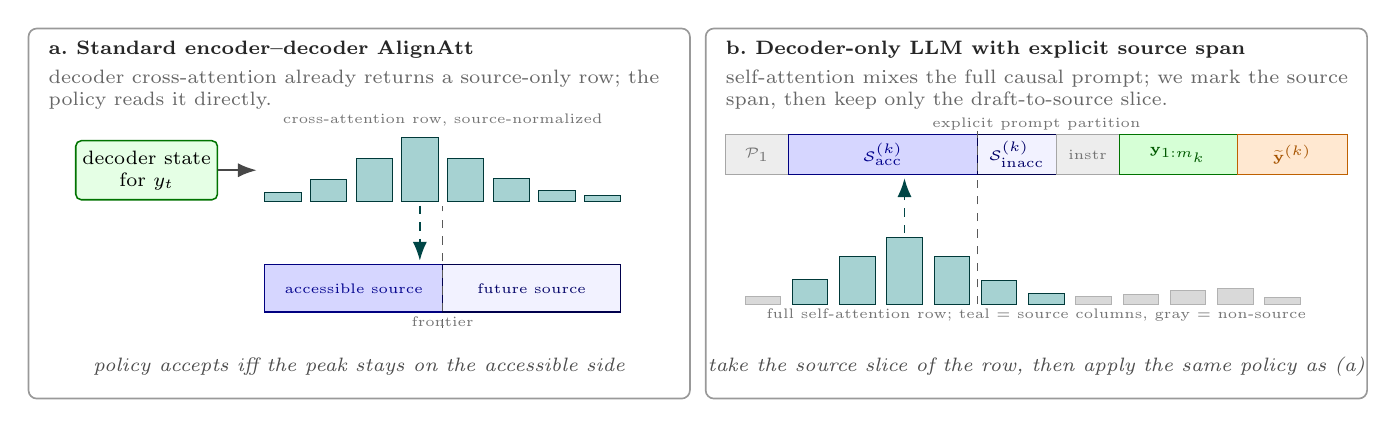
\begin{tikzpicture}[
  x=1cm, y=1cm,
  >={Latex[length=2.4mm]},
  every node/.style={font=\small, inner sep=0pt},
  panel/.style={draw=black!40, rounded corners=3pt, line width=0.6pt, fill=white},
  title/.style={font=\scriptsize\bfseries, text=black!85, align=left, inner sep=0pt},
  sub/.style={font=\scriptsize, text=black!60, align=left, inner sep=0pt},
  tny/.style={font=\tiny, text=black!55, align=center, inner sep=0pt},
  decbox/.style={draw=green!45!black, fill=green!10, rounded corners=2pt,
                 line width=0.55pt, inner sep=2pt, font=\scriptsize, align=center},
  caption/.style={font=\tiny, text=green!28!black, align=center, inner sep=0pt},
  flow/.style={->, draw=black!72, line width=0.85pt},
  peakflow/.style={->, draw=teal!55!black, line width=0.7pt, dashed},
  srcacc/.style={draw=blue!50!black, fill=blue!16, line width=0.4pt},
  srcinacc/.style={draw=blue!30!black, fill=blue!5, line width=0.4pt},
  prompt/.style={draw=black!35, fill=black!7, line width=0.35pt},
  tgtpref/.style={draw=green!45!black, fill=green!16, line width=0.35pt},
  draft/.style={draw=orange!75!black, fill=orange!18, line width=0.35pt},
]

  %% ================================================================
  %% LEFT PANEL: a. Standard encoder--decoder AlignAtt
  %% ================================================================
  \def\aL{0.00}\def\aR{8.40}\def\aB{1.50}\def\aT{6.20}
  \draw[panel] (\aL,\aB) rectangle (\aR,\aT);

  \node[title, anchor=north west] at (\aL+0.25,\aT-0.15)
    {a.~Standard encoder--decoder AlignAtt};
  \node[sub, anchor=north west, text width=7.90cm] at (\aL+0.25,\aT-0.52)
    {decoder cross-attention already returns a source-only row; the policy
     reads it directly.};

  % Decoder state box
  \node[decbox, minimum width=1.80cm, minimum height=0.75cm]
    (dec) at (1.50,4.40) {decoder state\\for $y_t$};

  % Histogram (cross-attention row over source frames) - 8 bars
  \def\aHx{3.00}        % left x of histogram
  \def\aHy{4.00}        % baseline y of histogram
  \def\aHw{0.46}        % bar width
  \def\aHg{0.12}        % gap between bars
  \def\aHs{0.58}        % step (width + gap)
  \foreach \i/\h in {0/0.12, 1/0.28, 2/0.55, 3/0.82, 4/0.55, 5/0.30, 6/0.14, 7/0.08} {
    \pgfmathsetmacro\x{\aHx + \aHs*\i}
    \filldraw[fill=teal!35, draw=teal!45!black, line width=0.25pt]
      (\x,\aHy) rectangle (\x+\aHw,\aHy+\h);
  }
  \pgfmathsetmacro\aHxR{\aHx + \aHs*7 + \aHw}   % right edge of histogram
  \node[tny, anchor=south] at ({(\aHx+\aHxR)/2}, {\aHy+0.95})
    {cross-attention row, source-normalized};

  % Arrow from decoder state to histogram
  \draw[flow] (dec.east) -- (\aHx-0.10,4.40);

  % Source bar below the histogram, aligned columnwise
  \def\aSyB{2.60}\def\aSyT{3.20}
  % peak bar x-position (bar 3, 0-indexed): bar left = aHx + aHs*3
  \pgfmathsetmacro\aPeakX{\aHx + \aHs*3 + \aHw/2}
  % frontier between bar 3 and bar 4: x = aHx + aHs*3 + aHw + aHg/2
  \pgfmathsetmacro\aFx{\aHx + \aHs*3 + \aHw + \aHg/2}
  \filldraw[srcacc] (\aHx,\aSyB) rectangle (\aFx,\aSyT);
  \filldraw[srcinacc] (\aFx,\aSyB) rectangle (\aHxR,\aSyT);
  \draw[black!65, dashed, line width=0.5pt] (\aFx,\aSyB-0.20) -- (\aFx,\aHy-0.05);

  \node[tny, text=blue!55!black] at ({(\aHx+\aFx)/2}, {(\aSyB+\aSyT)/2})
    {accessible source};
  \node[tny, text=blue!40!black] at ({(\aFx+\aHxR)/2}, {(\aSyB+\aSyT)/2})
    {future source};
  \node[tny, anchor=north] at (\aFx,\aSyB-0.05) {frontier};

  % Peak arrow (dashed teal) from peak bar down to accessible source
  \draw[peakflow] (\aPeakX,\aHy-0.05) -- (\aPeakX,\aSyT+0.05);

  % Caption (plain italic prose, close to figure)
  \node[font=\scriptsize\itshape, text=black!70, align=center]
    at ({(\aL+\aR)/2},1.90)
    {policy accepts iff the peak stays on the accessible side};

  %% ================================================================
  %% RIGHT PANEL: b. Decoder-only LLM with explicit source span
  %% ================================================================
  \def\bL{8.60}\def\bR{17.00}\def\bB{1.50}\def\bT{6.20}
  \draw[panel] (\bL,\bB) rectangle (\bR,\bT);

  \node[title, anchor=north west] at (\bL+0.25,\bT-0.15)
    {b.~Decoder-only LLM with explicit source span};
  \node[sub, anchor=north west, text width=7.90cm] at (\bL+0.25,\bT-0.52)
    {self-attention mixes the full causal prompt; we mark the source span,
     then keep only the draft-to-source slice.};

  % Prompt partition bar (horizontal, full width of visual area)
  \def\bPx{8.85}\def\bPxR{16.75}
  \def\bPyB{4.35}\def\bPyT{4.85}
  % Segment widths sum to bPxR - bPx = 7.90. Assign:
  %   P1=0.80, S_acc=2.40, S_inacc=1.00, instr=0.80, y_{1:m_k}=1.50, draft=1.40
  \def\bP1{0.80}\def\bSacc{2.40}\def\bSinacc{1.00}\def\bInstr{0.80}
  \def\bYpref{1.50}\def\bDraft{1.40}
  \pgfmathsetmacro\bx{\bPx}
  \filldraw[prompt] (\bx,\bPyB) rectangle ({\bx+\bP1},\bPyT);
  \node[tny] at ({\bx+\bP1/2},{(\bPyB+\bPyT)/2}) {$\mathcal{P}_1$};
  \pgfmathsetmacro\bx{\bPx + \bP1}
  \filldraw[srcacc] (\bx,\bPyB) rectangle ({\bx+\bSacc},\bPyT);
  \node[tny, text=blue!55!black] at ({\bx+\bSacc/2},{(\bPyB+\bPyT)/2})
    {$\mathcal{S}^{(k)}_{\mathrm{acc}}$};
  \pgfmathsetmacro\bx{\bPx + \bP1 + \bSacc}
  \pgfmathsetmacro\bFx{\bx}       % frontier x
  \filldraw[srcinacc] (\bx,\bPyB) rectangle ({\bx+\bSinacc},\bPyT);
  \node[tny, text=blue!40!black] at ({\bx+\bSinacc/2},{(\bPyB+\bPyT)/2})
    {$\mathcal{S}^{(k)}_{\mathrm{inacc}}$};
  \pgfmathsetmacro\bx{\bPx + \bP1 + \bSacc + \bSinacc}
  \filldraw[prompt] (\bx,\bPyB) rectangle ({\bx+\bInstr},\bPyT);
  \node[tny] at ({\bx+\bInstr/2},{(\bPyB+\bPyT)/2}) {instr};
  \pgfmathsetmacro\bx{\bPx + \bP1 + \bSacc + \bSinacc + \bInstr}
  \filldraw[tgtpref] (\bx,\bPyB) rectangle ({\bx+\bYpref},\bPyT);
  \node[tny, text=green!35!black] at ({\bx+\bYpref/2},{(\bPyB+\bPyT)/2})
    {$\mathbf{y}_{1:m_k}$};
  \pgfmathsetmacro\bx{\bPx + \bP1 + \bSacc + \bSinacc + \bInstr + \bYpref}
  \filldraw[draft] (\bx,\bPyB) rectangle ({\bx+\bDraft},\bPyT);
  \node[tny, text=orange!65!black] at ({\bx+\bDraft/2},{(\bPyB+\bPyT)/2})
    {$\widetilde{\mathbf{y}}^{(k)}$};

  \node[tny, anchor=south] at ({(\bPx+\bPxR)/2}, \bPyT+0.05)
    {explicit prompt partition};

  % Frontier dashed line through histogram+prompt bar (stops at histogram baseline 2.70)
  \draw[black!65, dashed, line width=0.5pt] (\bFx,2.70) -- (\bFx,\bPyT+0.05);

  % Self-attention histogram row below (one bar per rough segment-cell).
  % Show 12 cells spread across full width; source cells (S_acc + S_inacc) get teal,
  % everything else gets muted gray.  Bars visually indicate where the peak lies.
  \def\bHx{8.85}\def\bHxR{16.75}\def\bHyB{2.70}
  \def\bHw{0.45}\def\bHs{0.60}     % 12 cells * 0.60 = 7.20, fits in 7.90
  \def\bHxStart{9.10}
  % bar heights and source-mask (1 if source, 0 if not). Designed so peak lies on accessible source.
  % With 12 bars starting at x=9.10 step 0.60:
  %   bar0 x=9.10 (P1 area)       mask=0 h=0.10
  %   bar1 x=9.70 (S_acc start)   mask=1 h=0.32
  %   bar2 x=10.30 (S_acc)        mask=1 h=0.60
  %   bar3 x=10.90 (S_acc, peak)  mask=1 h=0.85
  %   bar4 x=11.50 (S_acc)        mask=1 h=0.60
  %   bar5 x=12.10 (near frontier)mask=1 h=0.30
  %   bar6 x=12.70 (S_inacc)      mask=1 h=0.14  -- to the right of frontier
  %   bar7 x=13.30 (instr)        mask=0 h=0.10
  %   bar8 x=13.90 (instr/y_pref) mask=0 h=0.12
  %   bar9 x=14.50 (y_pref)       mask=0 h=0.18
  %   bar10 x=15.10 (y_pref)      mask=0 h=0.20
  %   bar11 x=15.70 (draft)       mask=0 h=0.08
  \foreach \i/\h/\m in {
    0/0.10/0, 1/0.32/1, 2/0.60/1, 3/0.85/1, 4/0.60/1, 5/0.30/1,
    6/0.14/1, 7/0.10/0, 8/0.12/0, 9/0.18/0, 10/0.20/0, 11/0.08/0
  } {
    \pgfmathsetmacro\x{\bHxStart + \bHs*\i}
    \ifnum\m=1
      \filldraw[fill=teal!35, draw=teal!45!black, line width=0.25pt]
        (\x,\bHyB) rectangle (\x+\bHw,\bHyB+\h);
    \else
      \filldraw[fill=black!15, draw=black!30, line width=0.22pt]
        (\x,\bHyB) rectangle (\x+\bHw,\bHyB+\h);
    \fi
  }
  % Peak bar index 3: x=10.90, center at 10.90+0.225=11.125
  \pgfmathsetmacro\bPeakX{\bHxStart + \bHs*3 + \bHw/2}

  \node[tny, anchor=north] at ({(\bHx+\bHxR)/2}, \bHyB-0.05)
    {full self-attention row; teal = source columns, gray = non-source};

  % Peak arrow (teal dashed) from histogram peak up to prompt partition (indicating draft attends to acc source)
  \draw[peakflow] (\bPeakX, \bHyB+0.90) -- (\bPeakX, \bPyB-0.05);

  % Caption (plain italic prose, close to figure)
  \node[font=\scriptsize\itshape, text=black!70, align=center]
    at ({(\bL+\bR)/2},1.90)
    {take the source slice of the row, then apply the same policy as (a)};

\end{tikzpicture}
}%
\caption{\textbf{How AlignAtt changes substrate between encoder--decoder and
decoder-only models.} \emph{(a)} In the original encoder--decoder setting,
the decoder already exposes a source-only cross-attention row, so the policy
can gate tokens directly against the accessible source frontier: if the peak
of the row falls on the accessible side, the draft token is accepted.
\emph{(b)} In our decoder-only MT setting, source and target history share
one causal prompt. We therefore mark the source span explicitly in prompt
space, isolate translation-specific heads, and reconstruct only the
draft-to-source slice needed by the policy; the decision rule is otherwise
the same as in (a).}
\label{fig:alignatt-substrates}
\end{figure*}


\section{Submitted System Overview}
\label{sec:system}

\paragraph{ASR backend.}
The speech side of the submitted cascade uses Qwen3-ASR with the Qwen3 forced
aligner \citep{qwen3asr25}. For each chunk boundary, it returns an updated
transcript prefix together with per-word end times. We retain this dedicated
aligner because it is materially better than the discarded all-Gemma ASR path
on boundary accuracy, word error rate, and runtime; the auxiliary comparison is
reported in Appendix~\ref{sec:appendix-asr}.

\paragraph{MT backend.}
The translation side uses Gemma-4 E4B-it served through graph-compiled vLLM.
At step $k$, Gemma receives the current transcript prefix, the already accepted
target prefix, and a fixed translation instruction, then generates a short
draft continuation. AlignAtt accepts the longest draft prefix whose alignment
signal stays on the currently accessible side of the source frontier.

\paragraph{Streaming loop.}
The cascade is synchronous and chunk-based. Each chunk first updates the ASR
transcript prefix, then launches one MT request. Source words are considered
accessible only once their end time is older than a small hold-back margin. MT
output is append-only: once a target token is accepted, it is reused as causal
prefill for the next MT step and is never retracted.

\paragraph{Submitted operating points.}
We keep two official frozen submission regimes. The low-latency submission
uses $\Delta_{\mathrm{chunk}}=850$ ms together with the historical MT rewind
policy, and the high-latency submission uses $\Delta_{\mathrm{chunk}}=1500$ ms.
Both share the same ASR backend, Gemma-4 MT backbone, and MT-side AlignAtt
realization; only the operating point changes. Section~\ref{sec:main-results}
then reports separately a cleaner EN$\to$DE rerun at $\Delta_{\mathrm{chunk}}
=1100$ ms, without the MT rewind policy, which we use to track the current
maintained preset near the 2\,s boundary.

\begin{figure*}[t]
\centering
\resizebox{\linewidth}{!}{%
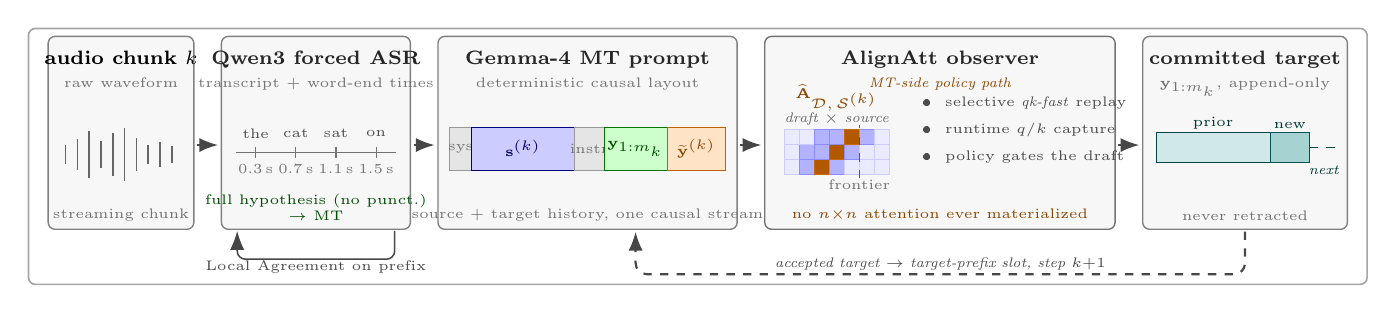
\begin{tikzpicture}[
  x=1cm, y=1cm,
  >={Latex[length=2.4mm]},
  every node/.style={font=\scriptsize, inner sep=0pt},
  panel/.style={draw=black!35, rounded corners=2.5pt, line width=0.6pt, fill=white},
  box/.style       ={draw=black!50,        rounded corners=2.5pt, line width=0.5pt,  fill=white},
  audiobox/.style  ={box, draw=black!50,   fill=black!3},
  asrbox/.style    ={box, draw=black!50, fill=black!3},
  mtbox/.style     ={box, draw=black!50,  fill=black!3},
  obsbox/.style    ={box, draw=black!55, fill=black!3},
  outbox/.style    ={box, draw=black!50,  fill=black!3},
  hdr/.style       ={font=\scriptsize\bfseries, align=center, inner sep=0pt},
  sub/.style       ={font=\tiny, text=black!55, align=center, inner sep=0pt},
  tagL/.style      ={font=\tiny, text=black!70, align=left,   inner sep=0pt},
  arr/.style       ={->, line width=0.9pt, draw=black!72},
  feed/.style      ={->, line width=0.8pt, draw=black!72, dashed},
  chunktick/.style ={draw=black!45, line width=0.5pt},
]

  %% ========================================================
  %% Canvas
  %% ========================================================
  \def\Wmax{17.00}\def\Hmax{3.25}
  \draw[panel] (0,0) rectangle (\Wmax,\Hmax);

  \begin{scope}[yshift=-1.15cm]

  %% ========================================================
  %% Main band: 5 processing stages
  %% ========================================================
  \def\bYB{1.85}\def\bYT{4.30}

  \def\aL{0.25}\def\aR{2.10}    % audio
  \def\bL{2.45}\def\bR{4.85}    % ASR
  \def\cL{5.20}\def\cR{9.00}    % MT prompt
  \def\dL{9.35}\def\dR{13.80}   % Observer (hero)
  \def\eL{14.15}\def\eR{16.75}  % committed target

  %% ---- Stage 1: Audio chunk ----
  \filldraw[audiobox] (\aL,\bYB) rectangle (\aR,\bYT);
  \node[hdr, anchor=north] at ({(\aL+\aR)/2},\bYT-0.18)
    {audio chunk $k$};
  \node[sub, anchor=north] at ({(\aL+\aR)/2},\bYT-0.52)
    {raw waveform};
  \def\awY{2.80}
  \foreach \i/\h in {0/0.35, 1/0.55, 2/0.85, 3/0.50, 4/0.78, 5/0.95,
                     6/0.60, 7/0.35, 8/0.45, 9/0.30} {
    \pgfmathsetmacro\xw{\aL+0.22 + 0.15*\i}
    \pgfmathsetmacro\yA{\awY - \h/2*0.70}
    \pgfmathsetmacro\yB{\awY + \h/2*0.70}
    \draw[black!60, line width=0.55pt] (\xw,\yA) -- (\xw,\yB);
  }
  \node[sub, anchor=south] at ({(\aL+\aR)/2},\bYB+0.10)
    {streaming chunk};

  %% ---- Stage 2: Qwen3 ASR ----
  \filldraw[asrbox] (\bL,\bYB) rectangle (\bR,\bYT);
  \node[hdr, text=black!85, anchor=north] at ({(\bL+\bR)/2},\bYT-0.18)
    {Qwen3 forced ASR};
  \node[sub, anchor=north] at ({(\bL+\bR)/2},\bYT-0.52)
    {transcript $+$ word-end times};
  \def\asrY{2.95}
  \def\asrLx{2.63}\def\asrRx{4.67}
  \draw[black!55, line width=0.4pt] (\asrLx,\asrY-0.12) -- (\asrRx,\asrY-0.12);
  \foreach \i/\tok in {0/the, 1/cat, 2/sat, 3/on} {
    \pgfmathsetmacro\xtk{\asrLx + 0.51*\i + 0.255}
    \node[font=\tiny, text=black!70] at (\xtk,\asrY+0.12) {\tok};
    \draw[black!55, line width=0.4pt] (\xtk,\asrY-0.05) -- (\xtk,\asrY-0.19);
  }
  \foreach \i/\lab in {0/{0.3}, 1/{0.7}, 2/{1.1}, 3/{1.5}} {
    \pgfmathsetmacro\xtk{\asrLx + 0.51*\i + 0.255}
    \node[font=\tiny, text=black!55] at (\xtk,\asrY-0.34) {\lab\,s};
  }
  \node[sub, anchor=south, text=green!30!black, align=center]
    at ({(\bL+\bR)/2},\bYB+0.10)
    {full hypothesis (no punct.)\\ $\to$ MT};

  % Local Agreement self-loop on Qwen3 ASR box (below)
  \draw[->, draw=black!72, line width=0.55pt, rounded corners=3pt]
    ({\bR-0.20},\bYB-0.02)
    -- ({\bR-0.20},\bYB-0.38)
    -- ({\bL+0.20},\bYB-0.38)
    -- ({\bL+0.20},\bYB-0.02);
  \node[font=\tiny, text=black!70, anchor=north]
    at ({(\bL+\bR)/2},\bYB-0.40)
    {Local Agreement on prefix};

  %% ---- Stage 3: MT prompt with explicit layout ----
  \filldraw[mtbox] (\cL,\bYB) rectangle (\cR,\bYT);
  \node[hdr, text=black!85, anchor=north] at ({(\cL+\cR)/2},\bYT-0.18)
    {Gemma-4 MT prompt};
  \node[sub, anchor=north] at ({(\cL+\cR)/2},\bYT-0.52)
    {deterministic causal layout};
  % Wider segmented bar; tiny labels use short forms (full names in caption)
  \def\pbL{5.35}\def\pbR{8.85}
  \def\pbB{2.60}\def\pbT{3.15}
  % widths (sum = 3.50): sys=0.28, src=1.30, instr=0.38, y_pref=0.80, draft=0.74
  \def\segsys{0.28}\def\segsrc{1.30}\def\segins{0.38}
  \def\segypref{0.80}\def\segdraft{0.74}
  \pgfmathsetmacro\xs{\pbL}
  \filldraw[draw=black!40, fill=black!10, line width=0.3pt]
    (\xs,\pbB) rectangle ({\xs+\segsys},\pbT);
  \node[font=\tiny, text=black!55] at ({\xs+\segsys/2},{(\pbB+\pbT)/2}) {sys};
  \pgfmathsetmacro\xs{\pbL+\segsys}
  \filldraw[draw=blue!50!black, fill=blue!20, line width=0.3pt]
    (\xs,\pbB) rectangle ({\xs+\segsrc},\pbT);
  \node[font=\tiny, text=blue!40!black] at ({\xs+\segsrc/2},{(\pbB+\pbT)/2})
    {$\mathbf{s}^{(k)}$};
  \pgfmathsetmacro\xs{\pbL+\segsys+\segsrc}
  \filldraw[draw=black!40, fill=black!10, line width=0.3pt]
    (\xs,\pbB) rectangle ({\xs+\segins},\pbT);
  \node[font=\tiny, text=black!55] at ({\xs+\segins/2},{(\pbB+\pbT)/2}) {instr};
  \pgfmathsetmacro\xs{\pbL+\segsys+\segsrc+\segins}
  \pgfmathsetmacro\ypSlotCx{\xs+\segypref/2}  % store target-prefix center for feedback
  \filldraw[draw=green!45!black, fill=green!20, line width=0.3pt]
    (\xs,\pbB) rectangle ({\xs+\segypref},\pbT);
  \node[font=\tiny, text=green!30!black] at ({\xs+\segypref/2},{(\pbB+\pbT)/2})
    {$\mathbf{y}_{1:m_k}$};
  \pgfmathsetmacro\xs{\pbL+\segsys+\segsrc+\segins+\segypref}
  \filldraw[draw=orange!75!black, fill=orange!22, line width=0.3pt]
    (\xs,\pbB) rectangle ({\xs+\segdraft},\pbT);
  \node[font=\tiny, text=orange!55!black] at ({\xs+\segdraft/2},{(\pbB+\pbT)/2})
    {$\widetilde{\mathbf{y}}^{(k)}$};
  \node[sub, anchor=south] at ({(\cL+\cR)/2},\bYB+0.10)
    {source $+$ target history, one causal stream};

  %% ---- Stage 4: AlignAtt observer (HERO) ----
  \filldraw[obsbox] (\dL,\bYB) rectangle (\dR,\bYT);
  \node[hdr, text=black!85, anchor=north] at ({(\dL+\dR)/2},\bYT-0.18)
    {AlignAtt observer};
  \node[sub, anchor=north, font=\tiny\itshape, text=orange!55!black]
    at ({(\dL+\dR)/2},\bYT-0.52)
    {MT-side policy path};
  % Mini attention matrix (3 rows draft x 7 cols source)
  \def\matL{9.60}\def\matB{2.55}
  \def\cellw{0.19}
  \foreach \r/\c/\k in {
    0/0/0, 0/1/1, 0/2/2, 0/3/1, 0/4/0, 0/5/0, 0/6/0,
    1/0/0, 1/1/1, 1/2/1, 1/3/2, 1/4/1, 1/5/0, 1/6/0,
    2/0/0, 2/1/0, 2/2/1, 2/3/1, 2/4/2, 2/5/1, 2/6/0
  } {
    \pgfmathsetmacro\xc{\matL + \c*\cellw}
    \pgfmathsetmacro\yc{\matB + \r*\cellw}
    \ifnum\k=2
      \filldraw[fill=orange!70!black, draw=orange!80!black, line width=0.18pt]
        (\xc,\yc) rectangle ({\xc+\cellw},{\yc+\cellw});
    \else\ifnum\k=1
      \filldraw[fill=blue!30, draw=blue!45, line width=0.18pt]
        (\xc,\yc) rectangle ({\xc+\cellw},{\yc+\cellw});
    \else
      \filldraw[fill=blue!8, draw=blue!20, line width=0.18pt]
        (\xc,\yc) rectangle ({\xc+\cellw},{\yc+\cellw});
    \fi\fi
  }
  % frontier marker between col 4 and col 5 (no label, stays inside matrix)
  \pgfmathsetmacro\frX{\matL + 5*\cellw}
  \draw[black!65, dashed, line width=0.45pt]
    (\frX,\matB-0.05) -- (\frX,{\matB+3*\cellw+0.05});
  % matrix title (above cells): formula + description on separate lines
  \node[font=\tiny\bfseries, text=orange!55!black, anchor=south]
    at ({\matL+7*\cellw/2},{\matB+3*\cellw+0.22})
    {$\widehat{\mathbf{A}}_{\mathcal{D},\,\mathcal{S}^{(k)}}$};
  \node[font=\tiny\itshape, text=black!60, anchor=south]
    at ({\matL+7*\cellw/2},{\matB+3*\cellw+0.04})
    {draft $\times$ source};
  % frontier caption below matrix (centered under the dashed line)
  \node[font=\tiny, text=black!55, anchor=north]
    at (\frX,\matB-0.06) {frontier};

  % Right column: 2 short properties (condensed)
  \def\hintX{11.35}
  \node[tagL, anchor=west] at (\hintX,3.45)
    {\textbullet\ \ selective \emph{qk-fast} replay};
  \node[tagL, anchor=west] at (\hintX,3.11)
    {\textbullet\ \ runtime $q/k$ capture};
  \node[tagL, anchor=west] at (\hintX,2.77)
    {\textbullet\ \ policy gates the draft};
  \node[sub, anchor=south, text=orange!55!black] at ({(\dL+\dR)/2},\bYB+0.10)
    {no $n{\times}n$ attention ever materialized};

  %% ---- Stage 5: Committed target ----
  \filldraw[outbox] (\eL,\bYB) rectangle (\eR,\bYT);
  \node[hdr, text=black!85, anchor=north] at ({(\eL+\eR)/2},\bYT-0.18)
    {committed target};
  \node[sub, anchor=north] at ({(\eL+\eR)/2},\bYT-0.52)
    {$\mathbf{y}_{1:m_k}$, append-only};
  \def\gbL{14.32}\def\gbR{16.60}
  \def\gbY{2.70}\def\gbH{0.38}
  \filldraw[draw=teal!55!black, fill=teal!18, line width=0.3pt]
    (\gbL,\gbY) rectangle ({\gbL+1.45},{\gbY+\gbH});
  \filldraw[draw=teal!65!black, fill=teal!35, line width=0.3pt]
    ({\gbL+1.45},\gbY) rectangle ({\gbL+1.95},{\gbY+\gbH});
  \draw[dashed, draw=teal!55!black, line width=0.3pt]
    ({\gbL+1.95},{\gbY+\gbH/2}) -- (\gbR,{\gbY+\gbH/2});
  \node[font=\tiny, text=teal!40!black, anchor=south]
    at ({\gbL+0.725},\gbY+\gbH+0.04) {prior};
  \node[font=\tiny, text=teal!45!black, anchor=south]
    at ({\gbL+1.70},\gbY+\gbH+0.04) {new};
  \node[font=\tiny, text=teal!40!black, anchor=north, font=\tiny\itshape]
    at ({\gbR-0.15},\gbY-0.04) {next};
  \node[sub, anchor=south] at ({(\eL+\eR)/2},\bYB+0.10)
    {never retracted};

  %% ========================================================
  %% Arrows between stages (clean, no labels)
  %% ========================================================
  \def\midY{2.92}
  \draw[arr] ({\aR+0.04},\midY) -- ({\bL-0.04},\midY);
  \draw[arr] ({\bR+0.04},\midY) -- ({\cL-0.04},\midY);
  \draw[arr] ({\cR+0.04},\midY) -- ({\dL-0.04},\midY);
  \draw[arr] ({\dR+0.04},\midY) -- ({\eL-0.04},\midY);

  %% ========================================================
  %% Feedback: committed target -> target-prefix slot of next step
  %% ========================================================
  \def\fbY{1.28}
  \draw[feed, rounded corners=4pt]
    ({(\eL+\eR)/2},\bYB-0.03)
    -- ({(\eL+\eR)/2},\fbY)
    -- (\ypSlotCx,\fbY)
    -- (\ypSlotCx,\bYB-0.03);
  \node[font=\tiny\itshape, text=black!70, anchor=south]
    at ({(\ypSlotCx+(\eL+\eR)/2)/2},\fbY+0.04)
    {accepted target $\rightarrow$ target-prefix slot, step $k{+}1$};

  \end{scope}

\end{tikzpicture}
}%
\caption{\textbf{Submitted cascade, one chunk-synchronous step.} Each chunk
first updates the source prefix with Qwen3 forced ASR, then runs one Gemma-4
MT step. The MT prompt keeps the ASR transcript explicit inside the
decoder-only causal layout, so the observer can capture the
selected heads' queries and keys on the deployed vLLM path and reconstruct only
the draft-to-source block
$\widehat{\mathbf{A}}_{\mathcal{D},\mathcal{S}^{(k)}}$ used by the acceptance
policy. Accepted target tokens are appended to $\mathbf{y}_{1:m_k}$ and become
the target-prefix slot of the next step's prompt (dashed teal feedback).}
\label{fig:system}
\end{figure*}


\section{Engine-Native AlignAtt for LLMs}
\label{sec:method}

This section focuses on the MT-side mechanism that makes Gemma-4 a usable
AlignAtt backend inside the retained cascade.

\subsection{Prompt Layout and Alignment Heads}

Standard AlignAtt does not directly apply because a decoder-only LLM has no
decoder cross-attention. We therefore recover a source-conditioned view by
forcing a deterministic prompt layout:
\begin{equation}
\mathbf{p}^{(k)} =
\left[\mathbf{p}^{\mathrm{sys}}
\Vert \mathbf{s}^{(k)}
\Vert \mathbf{p}^{\mathrm{instr}}, \mathbf{y}_{1:m_k}
\Vert \widetilde{\mathbf{y}}^{(k)}\right],
\label{eq:mt-prompt}
\end{equation}
where $\mathbf{s}^{(k)}$ is the live transcript prefix returned by ASR,
$\mathbf{y}_{1:m_k}$ is the already accepted translation prefix, and
$\widetilde{\mathbf{y}}^{(k)}$ is the draft proposed by Gemma-4 at the current
step. The transcript prefix is therefore a contiguous prompt span with a known
map $\phi^{(k)}$ from source-word indices to prompt positions.

Not all self-attention heads carry a useful translation signal
\citep{tokenheads26}. We score Gemma heads offline on held-out word-aligned MT
examples under this exact prompt layout and retain the top $k=8$ heads per
language pair. This head set is fixed at inference time and is the only part
of the policy that depends on offline calibration.
Appendix~\ref{sec:appendix-alignatt} reports the calibration table and the full
layer-head score maps.

\subsection{Selective Reconstruction for the Policy}

The policy never needs the full $n\times n$ self-attention matrix. It only
needs draft rows against source columns. For selected heads $(\ell,h)$, draft
positions $t$, and source positions $s$, we reconstruct
\begin{equation}
\widehat{A}^{(\ell,h)}_{t,s}
=
\frac{\exp\!\left(q^{(\ell,h)}_t \cdot k^{(\ell,h)}_{\phi^{(k)}(s)}\right)}
{\sum_j \exp\!\left(q^{(\ell,h)}_t \cdot k^{(\ell,h)}_j + m_{t,j}\right)},
\label{eq:mt-qk-fast}
\end{equation}
where the denominator still ranges over the entire prompt. We call this replay
path \emph{qk-fast}: it is exact up to floating-point reassociation relative to
the fused forward and only reconstructs the policy-visible block.

\begin{figure*}[t]
\centering
\resizebox{\linewidth}{!}{%
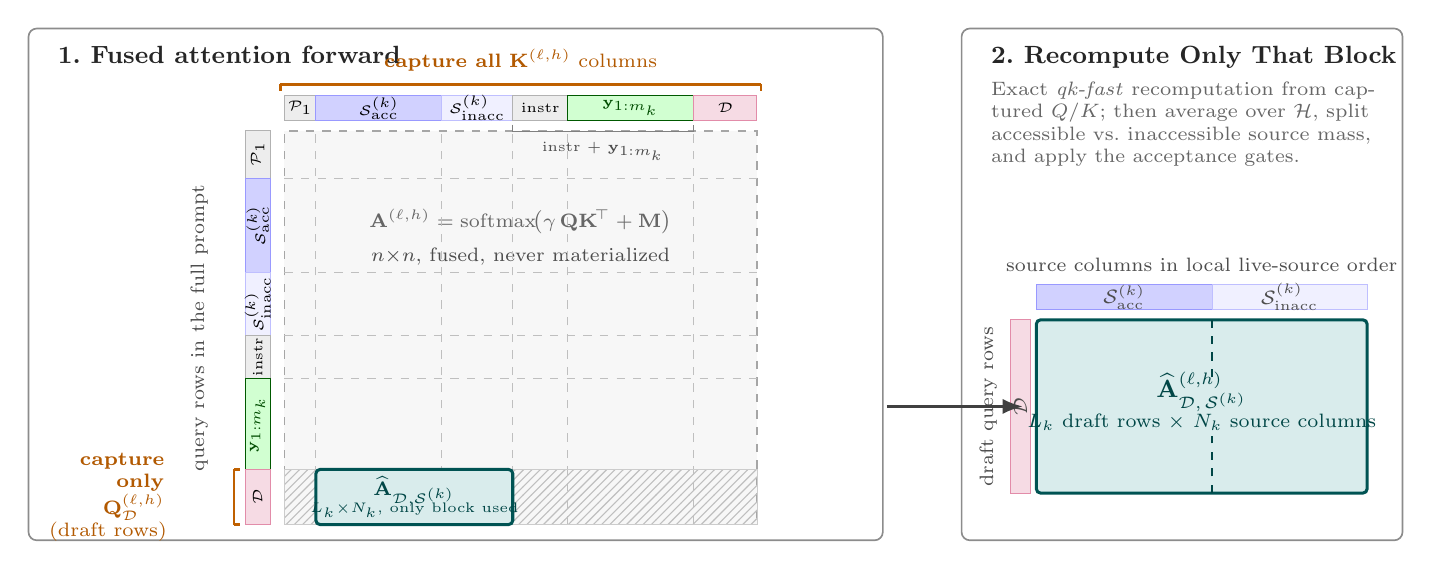
\begin{tikzpicture}[
  x=1cm, y=1cm,
  >={Latex[length=2.6mm]},
  every node/.style={font=\small},
  panel/.style={draw=black!45, rounded corners=3pt, line width=0.6pt, fill=white},
  title/.style={font=\bfseries\small, text=black!85},
  subtitle/.style={font=\scriptsize, text=black!60, align=left},
  stagearrow/.style={->, line width=1.1pt, draw=black!75},
  guide/.style={draw=black!25, line width=0.35pt, dashed},
  kernelbox/.style={draw=black!35, dashed, fill=black!3, line width=0.6pt},
  captureband/.style={fill=orange!20, draw=orange!75!black, line width=0.9pt},
  captureline/.style={draw=orange!75!black, line width=0.9pt, rounded corners=1pt},
  reconbox/.style={draw=teal!65!black, fill=teal!15, line width=1.1pt, rounded corners=1.5pt},
  partP/.style={draw=black!30, fill=black!7, line width=0.3pt},
  partPy/.style={draw=green!35!black, fill=green!18, line width=0.3pt},
  partSa/.style={draw=blue!40, fill=blue!18, line width=0.3pt},
  partSi/.style={draw=blue!25, fill=blue!6, line width=0.3pt},
  partD/.style={draw=purple!45, fill=purple!14, line width=0.3pt},
  notrecon/.style={pattern=north east lines, pattern color=black!25, draw=black!20, line width=0.2pt},
  labelnote/.style={font=\scriptsize, text=black!70, align=center},
  mathnote/.style={font=\scriptsize\itshape, text=black!60, align=center},
]

  \draw[panel] (-1.55, 0.35) rectangle (9.3, 6.85);
  \node[title, anchor=north west] at (-1.30, 6.75) {1.~Fused attention forward};

  \def\mL{1.70}\def\mR{7.70}\def\mB{0.55}\def\mT{5.55}
  \def\cPa{2.10}
  \def\cSa{3.70}
  \def\cSi{4.60}
  \def\cPi{5.30}
  \def\cPy{6.90}
  \def\rPa{4.95}
  \def\rSa{3.75}
  \def\rSi{2.95}
  \def\rPi{2.40}
  \def\rPy{1.25}

  \draw[kernelbox] (\mL, \mB) rectangle (\mR, \mT);
  \node[mathnote] at ({(\mL+\mR)/2}, 4.40)
    {$\mathbf{A}^{(\ell,h)}=\mathrm{softmax}\!\bigl(\gamma\,\mathbf{Q}\mathbf{K}^{\!\top}+\mathbf{M}\bigr)$};
  \node[labelnote] at ({(\mL+\mR)/2}, 3.95) {$n{\times}n$, fused, never materialized};

  \foreach \x in {\cPa,\cSa,\cSi,\cPi,\cPy} \draw[guide] (\x,\mB) -- (\x,\mT);
  \foreach \y in {\rPa,\rSa,\rSi,\rPi,\rPy} \draw[guide] (\mL,\y) -- (\mR,\y);

  \draw[notrecon] (\mL,  \mB) rectangle (\cPa,  \rPy);
  \draw[notrecon] (\cSi, \mB) rectangle (\mR,   \rPy);

  \draw[reconbox] (\cPa, \mB) rectangle (\cSi, \rPy);
  \node[font=\scriptsize\bfseries, text=teal!55!black]
    at ({(\cPa+\cSi)/2}, {(\mB+\rPy)/2 + 0.07})
    {$\widehat{\mathbf{A}}_{\mathcal{D},\mathcal{S}^{(k)}}$};
  \node[font=\tiny, text=teal!55!black]
    at ({(\cPa+\cSi)/2}, {(\mB+\rPy)/2 - 0.17})
    {$L_k{\times}N_k$, only block used};

  \def\csB{5.68}\def\csT{6.00}
  \draw[partP ] (\mL  ,\csB) rectangle (\cPa ,\csT) node[midway,font=\tiny]{$\mathcal{P}_1$};
  \draw[partSa] (\cPa ,\csB) rectangle (\cSa ,\csT) node[midway,font=\tiny]{$\mathcal{S}^{(k)}_{\mathrm{acc}}$};
  \draw[partSi] (\cSa ,\csB) rectangle (\cSi ,\csT) node[midway,font=\tiny]{$\mathcal{S}^{(k)}_{\mathrm{inacc}}$};
  \draw[partP ] (\cSi ,\csB) rectangle (\cPi,\csT) node[midway,font=\tiny]{instr};
  \draw[partPy] (\cPi,\csB) rectangle (\cPy,\csT) node[midway,font=\tiny,text=green!30!black]{$\mathbf{y}_{1:m_k}$};
  \draw[partD ] (\cPy,\csB) rectangle (\mR  ,\csT) node[midway,font=\tiny]{$\mathcal{D}$};
  \draw[black!50, line width=0.3pt] (\cSi, \csB-0.05) -- (\cSi, \csB-0.14) -- (\cPy, \csB-0.14) -- (\cPy, \csB-0.05);
  \node[labelnote, anchor=north, font=\tiny] at ({(\cSi+\cPy)/2}, \csB-0.15) {instr $+$ $\mathbf{y}_{1:m_k}$};
  \draw[captureline] ({\mL-0.05}, {\csT+0.14}) -- ({\mR+0.05}, {\csT+0.14});
  \draw[captureline] ({\mL-0.05}, {\csT+0.06}) -- ({\mL-0.05}, {\csT+0.14});
  \draw[captureline] ({\mR+0.05}, {\csT+0.06}) -- ({\mR+0.05}, {\csT+0.14});
  \node[labelnote, anchor=south] at ({(\mL+\mR)/2}, {\csT+0.18})
    {\textcolor{orange!70!black}{\textbf{capture all} $\mathbf{K}^{(\ell,h)}$ columns}};

  \def\rsL{1.20}\def\rsR{1.52}
  \draw[partP ] (\rsL,\rPa ) rectangle (\rsR,\mT  ) node[midway,rotate=90,font=\tiny]{$\mathcal{P}_1$};
  \draw[partSa] (\rsL,\rSa ) rectangle (\rsR,\rPa ) node[midway,rotate=90,font=\tiny]{$\mathcal{S}^{(k)}_{\mathrm{acc}}$};
  \draw[partSi] (\rsL,\rSi ) rectangle (\rsR,\rSa ) node[midway,rotate=90,font=\tiny]{$\mathcal{S}^{(k)}_{\mathrm{inacc}}$};
  \draw[partP ] (\rsL,\rPi) rectangle (\rsR,\rSi ) node[midway,rotate=90,font=\tiny]{instr};
  \draw[partPy] (\rsL,\rPy) rectangle (\rsR,\rPi) node[midway,rotate=90,font=\tiny,text=green!30!black]{$\mathbf{y}_{1:m_k}$};
  \draw[partD ] (\rsL,\mB  ) rectangle (\rsR,\rPy) node[midway,rotate=90,font=\tiny]{$\mathcal{D}$};
  \node[labelnote, rotate=90] at ({\rsL-0.58}, {(\mB+\mT)/2})
    {query rows in the full prompt};

  \draw[captureline] ({\rsL-0.14}, \mB) -- ({\rsL-0.14}, \rPy);
  \draw[captureline] ({\rsL-0.14}, \mB) -- ({\rsL-0.06}, \mB);
  \draw[captureline] ({\rsL-0.14}, \rPy) -- ({\rsL-0.06}, \rPy);
  \node[labelnote, text=orange!70!black, anchor=east, align=right, text width=1.55cm]
    at (0.30, {(\mB+\rPy)/2})
    {\textbf{capture only}\\ $\mathbf{Q}^{(\ell,h)}_{\mathcal{D}}$\\(draft rows)};

  \draw[panel] (10.3, 0.35) rectangle (15.9, 6.85);
  \node[title, anchor=north west] at (10.55, 6.75) {2.~Recompute Only That Block};
  \node[subtitle, anchor=north west, text width=5.05cm] at (10.55, 6.29)
    {Exact \emph{qk-fast} recomputation from captured $Q/K$; then average over $\mathcal{H}$, split accessible vs.\ inaccessible source mass, and apply the acceptance gates.};

  \def\bL{11.25}\def\bR{15.45}\def\bMid{13.48}
  \def\bB{0.95}\def\bT{3.15}
  \def\bcB{3.28}\def\bcT{3.60}

  \draw[partSa] (\bL,\bcB) rectangle (\bMid,\bcT);
  \node[labelnote] at ({(\bL+\bMid)/2}, {(\bcB+\bcT)/2}) {$\mathcal{S}^{(k)}_{\mathrm{acc}}$};
  \draw[partSi] (\bMid,\bcB) rectangle (\bR,\bcT);
  \node[labelnote] at ({(\bMid+\bR)/2}, {(\bcB+\bcT)/2}) {$\mathcal{S}^{(k)}_{\mathrm{inacc}}$};
  \node[labelnote, anchor=south] at ({(\bL+\bR)/2}, {\bcT+0.04})
    {source columns in local live-source order};

  \def\brL{10.92}\def\brR{11.18}
  \draw[partD] (\brL,\bB) rectangle (\brR,\bT);
  \node[labelnote, rotate=90] at ({(\brL+\brR)/2}, {(\bB+\bT)/2}) {$\mathcal{D}$};
  \node[labelnote, rotate=90] at (10.64, {(\bB+\bT)/2})
    {draft query rows};

  \draw[reconbox] (\bL,\bB) rectangle (\bR,\bT);
  \draw[teal!55!black, dashed, line width=0.4pt] (\bMid,\bB) -- (\bMid, 1.68);
  \draw[teal!55!black, dashed, line width=0.4pt] (\bMid, 2.42) -- (\bMid,\bT);
  \node[font=\small, text=teal!55!black]
    at ({(\bL+\bR)/2}, {(\bB+\bT)/2 + 0.18})
    {$\widehat{\mathbf{A}}^{(\ell,h)}_{\mathcal{D},\,\mathcal{S}^{(k)}}$};
  \node[labelnote, text=teal!55!black]
    at ({(\bL+\bR)/2}, {(\bB+\bT)/2 - 0.20})
    {$L_k$ draft rows $\times$ $N_k$ source columns};

  \draw[stagearrow]
    (9.35, {(\bB+\bT)/2})
    -- (11.08, {(\bB+\bT)/2});
\end{tikzpicture}
}%
\caption{\textbf{Selective reconstruction with engine-native capture.} The
$n{\times}n$ attention matrix
$\mathbf{A}^{(\ell,h)}$ is executed entirely inside the fused attention
kernel, so the full $n{\times}n$ matrix is never materialized. For each
AlignAtt head $(\ell,h)\in\mathcal{H}$, the observer copies
$\mathbf{K}^{(\ell,h)}$ for all positions and $\mathbf{Q}^{(\ell,h)}$ only for
the draft rows $\mathcal{D}$ into fixed-shape buffers. The green band
$\mathbf{y}_{1:m_k}$ marks the committed target prefix that grows across
chunks; hatched cells are never reconstructed. After the forward,
Eq.~\eqref{eq:mt-qk-fast} recomputes exactly only the draft-to-source block
$\widehat{\mathbf{A}}_{\mathcal{D},\mathcal{S}^{(k)}}$, which is the sole
object consumed by the source-side provenance split of
Eqs.~\eqref{eq:mt-prov-acc}--\eqref{eq:mt-provenance}, where
$\pi_t^{\mathrm{acc}}$ drives the gate and $\pi_t^{\mathrm{inacc}}$ is
retained for diagnostics, and by the acceptance policy of this section.}
\label{fig:qk-fast}
\end{figure*}


From these per-head rows we build two source-side provenance features for each
drafted token: accessible-source mass and inaccessible-source mass,
\begin{align}
  \pi_t^{\mathrm{acc}}
  &=
  \sum_{s \in \mathcal{S}^{(k)}_{\mathrm{acc}}} \bar{\mathbf{r}}_t(s),
  \label{eq:mt-prov-acc}\\
  \pi_t^{\mathrm{inacc}}
  &=
  \sum_{s \in \mathcal{S}^{(k)}_{\mathrm{inacc}}} \bar{\mathbf{r}}_t(s),
  \label{eq:mt-provenance}
\end{align}
where $\bar{\mathbf{r}}_t$ is the head-averaged reconstructed row. We
additionally normalize per-head rows online with prefix Welford statistics and
apply a short median filter along the source axis before taking the source-side
argmax. This stabilizes the alignment peak without changing the underlying
replayed rows.

\subsection{AlignAtt Acceptance Policy}

The submitted MT policy is a first-failure scan over drafted tokens. Let
$\hat{s}_t$ be the source-side argmax of the filtered row for draft token $t$,
and let $N^{(k)}_{\mathrm{acc}}$ be the number of source words whose ASR end
time is already on the accessible side of the frontier. The scan stops when one
of three conditions first fires:
\begin{align}
  \text{\textsc{source-frontier}} :\quad
  &\hat{s}_t \ge N^{(k)}_{\mathrm{acc}} + b,
  \label{eq:mt-stop-frontier}\\
  \text{\textsc{argmax-mass-weak}} :\quad
  &\bar{\mathbf{r}}_t(\hat{s}_t) < \tau_{\mathrm{argmax}},
  \label{eq:mt-stop-argmax}\\
  \text{\textsc{provenance-weak}} :\quad
  &\pi_t^{\mathrm{acc}} < \tau_{\mathrm{src}}.
  \label{eq:mt-stop-prov}
\end{align}
The first condition prevents dependence on still-inaccessible source words, the
second rejects weak alignment peaks, and the third rejects tokens with too
little total accessible-source support. The accepted output is the longest
draft prefix preceding the first failure, rounded back to the nearest
stability-unit boundary so partial subword fragments are never emitted. We
intentionally do not impose an anti-rewind rule on $\hat{s}_t$, because that
bias consistently hurt valid reorderings in EN$\to$ZH development.

Figure~\ref{fig:appendix-policy-pipeline} visualizes the full pipeline, from
the reconstructed block $\widehat{\mathbf{A}}^{(\ell,h)}_{t,s}$ to the
first-failure scan. Figure~\ref{fig:mt-selective-reconstruction} shows the
same gate on a live MT draft: black stars mark drafted tokens whose source
argmax stays on the accessible side of the frontier, and the first red star
marks the position at which the \textsc{source-frontier} condition fires.

\begin{figure*}[t]
\centering
\resizebox{\linewidth}{!}{%
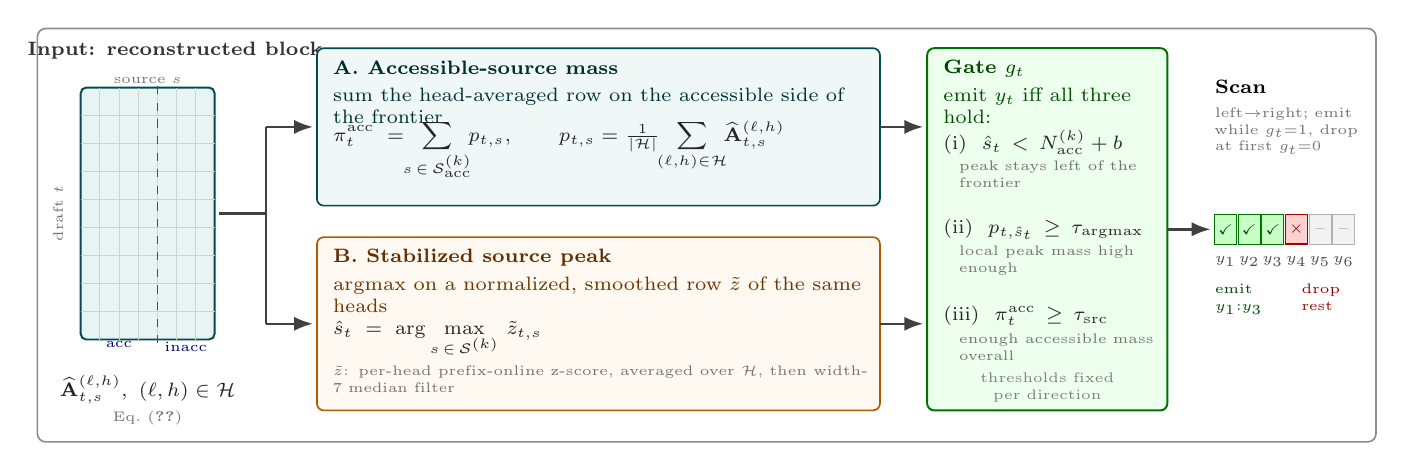
\begin{tikzpicture}[
  x=1cm, y=1cm,
  >={Latex[length=2.4mm]},
  every node/.style={font=\small, inner sep=0pt},
  panel/.style={draw=black!45, rounded corners=3pt, line width=0.6pt, fill=white},
  branchL/.style={draw=teal!60!black, line width=0.6pt, rounded corners=2.5pt,
                  fill=teal!6},
  branchR/.style={draw=orange!70!black, line width=0.6pt, rounded corners=2.5pt,
                  fill=orange!5},
  gatebox/.style={draw=green!45!black, line width=0.7pt, rounded corners=2.5pt,
                  fill=green!7},
  tensorbox/.style={draw=teal!60!black, line width=0.7pt, rounded corners=2pt,
                    fill=teal!9},
  flow/.style={->, draw=black!75, line width=0.9pt},
  sectitle/.style={font=\scriptsize\bfseries, align=left, inner sep=0pt},
  caption/.style={font=\scriptsize, align=left, text=black!60, inner sep=0pt},
  eqn/.style={font=\scriptsize, align=left, text=black!85, inner sep=0pt},
  sublab/.style={font=\tiny, align=left, text=black!55, inner sep=0pt},
  axlab/.style={font=\tiny, align=center, text=black!55, inner sep=0pt},
]

  \def\Wmax{17.00}\def\Hmax{5.25}
  \draw[panel] (0.00,0.00) rectangle (\Wmax,\Hmax);

  % === Input: reconstructed tensor block ===================================
  \def\ixL{0.55}\def\ixR{2.25}\def\iyB{1.30}\def\iyT{4.50}

  \node[sectitle, text=black!80, anchor=south]
    at ({(\ixL+\ixR)/2 + 0.35},\iyT+0.35)
    {Input: reconstructed block};

  \draw[tensorbox] (\ixL,\iyB) rectangle (\ixR,\iyT);
  \foreach \i in {1,...,8} {
    \pgfmathsetmacro\yy{\iyB + (\iyT-\iyB)*\i/9}
    \draw[black!18, line width=0.25pt] (\ixL,\yy) -- (\ixR,\yy);
  }
  \foreach \j in {1,...,6} {
    \pgfmathsetmacro\xx{\ixL + (\ixR-\ixL)*\j/7}
    \draw[black!18, line width=0.25pt] (\xx,\iyB) -- (\xx,\iyT);
  }
  \draw[black!70, dashed, line width=0.5pt]
    ({\ixL + (\ixR-\ixL)*4/7},\iyB-0.05)
    -- ({\ixL + (\ixR-\ixL)*4/7},\iyT+0.05);
  \node[axlab, anchor=south] at ({(\ixL+\ixR)/2}, \iyT+0.05) {source $s$};
  \node[axlab, rotate=90, anchor=south] at ({\ixL-0.22}, {(\iyB+\iyT)/2})
    {draft $t$};
  \node[axlab, text=blue!55!black, anchor=north]
    at ({\ixL + (\ixR-\ixL)*2/7}, \iyB-0.02) {acc};
  \node[axlab, text=blue!40!black, anchor=north]
    at ({\ixL + (\ixR-\ixL)*5.5/7}, \iyB-0.02) {inacc};
  \node[eqn, anchor=north] at ({(\ixL+\ixR)/2}, \iyB-0.45)
    {$\widehat{\mathbf{A}}^{(\ell,h)}_{t,s},\ (\ell,h)\in\mathcal{H}$};
  \node[sublab, anchor=north] at ({(\ixL+\ixR)/2}, \iyB-0.90)
    {Eq.~\eqref{eq:mt-qk-fast}};

  % --- Split arrow ---------------------------------------------------------
  \def\jx{2.90}
  \draw[flow, -] (\ixR+0.05,{(\iyB+\iyT)/2}) -- (\jx,{(\iyB+\iyT)/2});
  \draw[black!75, line width=0.85pt, -] (\jx,{(\iyB+\iyT)/2}) -- (\jx,4.00);
  \draw[black!75, line width=0.85pt, -] (\jx,{(\iyB+\iyT)/2}) -- (\jx,1.50);
  \draw[flow] (\jx,4.00) -- (3.50,4.00);
  \draw[flow] (\jx,1.50) -- (3.50,1.50);

  % === Branch A: Accessible-source mass ====================================
  \def\aL{3.55}\def\aR{10.70}\def\aB{3.00}\def\aT{5.00}
  \draw[branchL] (\aL,\aB) rectangle (\aR,\aT);

  \node[sectitle, text=teal!35!black, anchor=north west] at (\aL+0.20,\aT-0.15)
    {A.~Accessible-source mass};
  \node[caption, text=teal!40!black, anchor=north west,
        text width=6.75cm] at (\aL+0.20,\aT-0.50)
    {sum the head-averaged row on the accessible side of the frontier};

  \node[eqn, anchor=west] at (\aL+0.20,\aT-1.30)
    {$\displaystyle \pi^{\mathrm{acc}}_t\;=\!\!\sum_{s\,\in\,\mathcal{S}^{(k)}_{\mathrm{acc}}}\!\!p_{t,s},
      \qquad p_{t,s}=\tfrac{1}{|\mathcal{H}|}\!\!\sum_{(\ell,h)\in\mathcal{H}}\!\!\widehat{\mathbf{A}}^{(\ell,h)}_{t,s}$};

  \draw[flow] (\aR,{(\aB+\aT)/2}) -- (\aR+0.55,{(\aB+\aT)/2});

  % === Branch B: Stabilized peak ===========================================
  \def\bL{3.55}\def\bR{10.70}\def\bB{0.40}\def\bT{2.60}
  \draw[branchR] (\bL,\bB) rectangle (\bR,\bT);

  \node[sectitle, text=orange!38!black, anchor=north west] at (\bL+0.20,\bT-0.15)
    {B.~Stabilized source peak};
  \node[caption, text=orange!42!black, anchor=north west,
        text width=6.75cm] at (\bL+0.20,\bT-0.50)
    {argmax on a normalized, smoothed row $\tilde z$ of the same heads};

  \node[eqn, anchor=west] at (\bL+0.20,\bT-1.30)
    {$\displaystyle \hat s_t\;=\;\arg\max_{s\,\in\,\mathcal{S}^{(k)}}\,\tilde z_{t,s}$};
  \node[sublab, anchor=west, text width=6.75cm] at (\bL+0.20,\bT-1.80)
    {$\tilde z$: per-head prefix-online z-score, averaged over $\mathcal{H}$,
     then width-$7$ median filter};

  \draw[flow] (\bR,{(\bB+\bT)/2}) -- (\bR+0.55,{(\bB+\bT)/2});

  % === Gate ================================================================
  \def\gL{11.30}\def\gR{14.35}\def\gB{0.40}\def\gT{5.00}
  \draw[gatebox] (\gL,\gB) rectangle (\gR,\gT);

  \node[sectitle, text=green!28!black, anchor=north west] at (\gL+0.20,\gT-0.15)
    {Gate $g_t$};
  \node[caption, text=green!32!black, anchor=north west,
        text width=2.65cm] at (\gL+0.20,\gT-0.50)
    {emit $y_t$ iff all three hold:};

  \node[eqn, anchor=west] at (\gL+0.20,\gT-1.20)
    {(i)\ \ $\hat s_t \,<\, N^{(k)}_{\mathrm{acc}} + b$};
  \node[sublab, anchor=west, text width=2.50cm]
    at (\gL+0.40,\gT-1.60) {peak stays left of the frontier};

  \node[eqn, anchor=west] at (\gL+0.20,\gT-2.30)
    {(ii)\ \ $p_{t,\hat s_t}\,\ge\,\tau_{\mathrm{argmax}}$};
  \node[sublab, anchor=west, text width=2.50cm]
    at (\gL+0.40,\gT-2.70) {local peak mass high enough};

  \node[eqn, anchor=west] at (\gL+0.20,\gT-3.40)
    {(iii)\ \ $\pi^{\mathrm{acc}}_t\,\ge\,\tau_{\mathrm{src}}$};
  \node[sublab, anchor=west, text width=2.50cm]
    at (\gL+0.40,\gT-3.80) {enough accessible mass overall};

  \node[sublab, text=black!50, anchor=south, text width=2.65cm,
        align=center] at ({(\gL+\gR)/2},\gB+0.10)
    {thresholds fixed per direction};

  \draw[flow] (\gR,{(\gB+\gT)/2}) -- (\gR+0.55,{(\gB+\gT)/2});

  % === Scan ================================================================
  \def\sL{14.95}\def\sR{16.85}
  \node[sectitle, anchor=north west] at (\sL,4.60) {Scan};
  \node[sublab, anchor=north west, text width=1.85cm] at (\sL,4.25)
    {left$\to$right; emit while $g_t{=}1$, drop at first $g_t{=}0$};

  \def\cellw{0.28}\def\cellh{0.38}\def\cellg{0.02}
  \def\stX{\sL}
  \def\stY{2.51}
  \foreach \i in {0,1,2} {
    \pgfmathsetmacro\x{\stX + (\cellw+\cellg)*\i}
    \filldraw[fill=green!22, draw=green!45!black, line width=0.4pt]
      (\x,\stY) rectangle (\x+\cellw,\stY+\cellh);
    \node[font=\tiny, text=green!30!black, inner sep=0pt]
      at (\x+\cellw/2,\stY+\cellh/2) {\textbf{\checkmark}};
  }
  \pgfmathsetmacro\xf{\stX + (\cellw+\cellg)*3}
  \filldraw[fill=red!18, draw=red!65!black, line width=0.55pt]
    (\xf,\stY) rectangle (\xf+\cellw,\stY+\cellh);
  \node[font=\tiny, text=red!60!black, inner sep=0pt]
    at (\xf+\cellw/2,\stY+\cellh/2) {\textbf{$\times$}};
  \foreach \i in {4,5} {
    \pgfmathsetmacro\x{\stX + (\cellw+\cellg)*\i}
    \filldraw[fill=black!5, draw=black!30, line width=0.35pt]
      (\x,\stY) rectangle (\x+\cellw,\stY+\cellh);
    \node[font=\tiny, text=black!45, inner sep=0pt]
      at (\x+\cellw/2,\stY+\cellh/2) {--};
  }
  \foreach \i/\tok in {0/{$y_1$},1/{$y_2$},2/{$y_3$},3/{$y_4$},4/{$y_5$},5/{$y_6$}} {
    \pgfmathsetmacro\x{\stX + (\cellw+\cellg)*\i}
    \node[font=\tiny, text=black!70, inner sep=0pt]
      at (\x+\cellw/2,\stY-0.22) {\tok};
  }
  \node[sublab, text=green!30!black, anchor=north west, text width=1.1cm]
    at (\sL,\stY-0.50) {emit $y_1{:}y_3$};
  \node[sublab, text=red!60!black, anchor=north west, text width=0.9cm]
    at ({\sL+1.10},\stY-0.50) {drop rest};

\end{tikzpicture}
}%
\caption{\textbf{From the reconstructed block to an acceptance decision.}
The selective \emph{qk-fast} reconstruction produces
$\widehat{\mathbf{A}}^{(\ell,h)}_{t,s}$ for $(\ell,h)\in\mathcal{H}$, with draft
positions $t$ against source positions $s$ (left). The policy reads it through
two parallel aggregations. \emph{Branch~A} averages the selected heads into a
row $p_{t,\cdot}$ and sums its mass on the accessible side of the frontier,
giving the provenance score $\pi^{\mathrm{acc}}_t$. \emph{Branch~B} returns
the peak $\hat s_t$ of a stabilized row $\tilde z_{t,\cdot}$, where $\tilde
z$ is obtained by z-scoring each head with prefix-online Welford moments,
averaging over~$\mathcal{H}$, and applying a width-$7$ median filter along
the source axis. The gate $g_t$ accepts draft token $t$ iff the peak stays on
the accessible side of the frontier, the peak mass exceeds
$\tau_{\mathrm{argmax}}$, and the accessible-source mass exceeds
$\tau_{\mathrm{src}}$. A left-to-right scan emits the longest run of accepting
tokens and drops the remainder at the first failure.}
\label{fig:policy-pipeline}
\end{figure*}

\begin{figure*}[!tbp]
\centering
\resizebox{0.94\textwidth}{!}{%
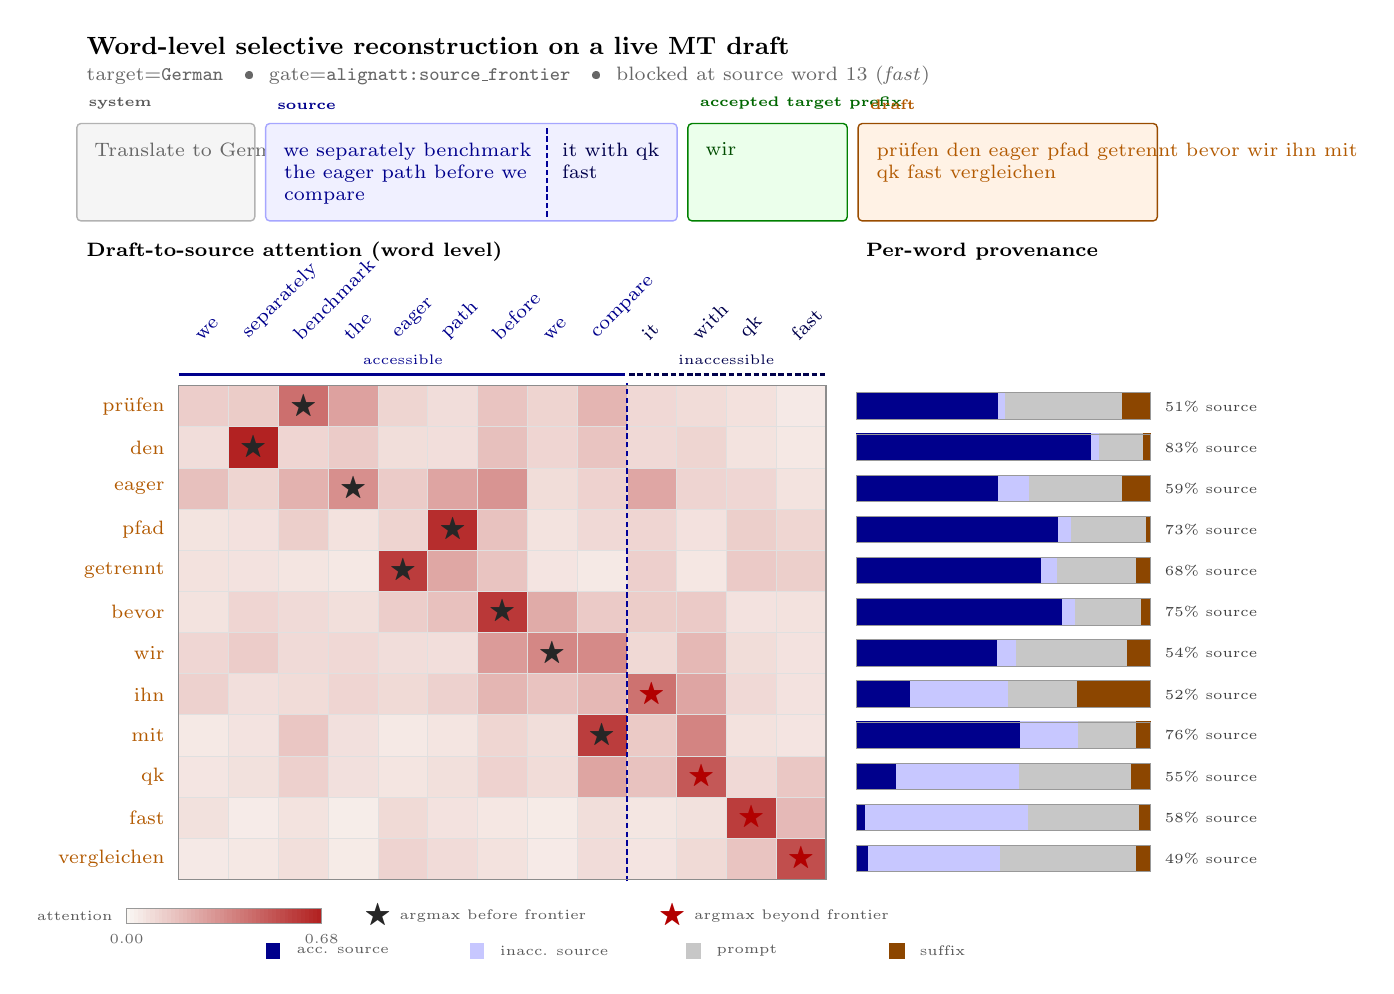
\begin{tikzpicture}[x=0.55cm,y=0.55cm, every node/.style={font=\scriptsize}]
\node[anchor=west, font=\bfseries\small] at (-0.15,21.45) {Word-level selective reconstruction on a live MT draft};
\node[anchor=west, text=black!60] at (-0.15,20.75) {target=\texttt{German} \; \textbullet \; gate=\texttt{alignatt:source\_frontier} \; \textbullet \; blocked at source word 13 (\emph{fast})};
\node[anchor=south west, font=\bfseries\tiny, text=black!65] at (-0.10,19.75) {system};
\draw[rounded corners=1.5pt, fill=black!4, draw=black!30, line width=0.5pt] (-0.15,17.40) rectangle (3.96,19.65);
\node[anchor=north west, text=black!60, align=left, text width=3.60cm] at (0.05,19.43) {Translate to German.};
\node[anchor=south west, font=\bfseries\tiny, text=blue!55!black] at (4.26,19.75) {source};
\draw[rounded corners=1.5pt, fill=blue!6, draw=blue!35, line width=0.5pt] (4.21,17.40) rectangle (13.71,19.65);
\node[anchor=north west, text=blue!55!black, align=left, text width=3.39cm] at (4.41,19.43) {we separately benchmark the eager path before we compare};
\draw[draw=blue!60!black, dash pattern=on 2pt off 1pt, line width=0.7pt] (10.71,17.50) -- (10.71,19.55);
\node[anchor=north west, text=blue!30!black, align=left, text width=1.46cm] at (10.83,19.43) {it with qk fast};
\node[anchor=south west, font=\bfseries\tiny, text=green!40!black] at (14.01,19.75) {accepted target prefix};
\draw[rounded corners=1.5pt, fill=green!8, draw=green!50!black, line width=0.5pt] (13.96,17.40) rectangle (17.64,19.65);
\node[anchor=north west, text=green!30!black, align=left, text width=1.80cm] at (14.16,19.43) {wir};
\node[anchor=south west, font=\bfseries\tiny, text=orange!70!black] at (17.94,19.75) {draft};
\draw[rounded corners=1.5pt, fill=orange!10, draw=orange!60!black, line width=0.5pt] (17.89,17.40) rectangle (24.80,19.65);
\node[anchor=north west, text=orange!70!black, align=left, text width=6.10cm] at (18.09,19.43) {pr\"ufen den eager pfad getrennt bevor wir ihn mit qk fast vergleichen};
\node[anchor=west, font=\bfseries\scriptsize] at (-0.15,16.70) {Draft-to-source attention (word level)};
\node[anchor=west, font=\bfseries\scriptsize] at (17.85,16.70) {Per-word provenance};
\node[anchor=south west, rotate=45, text=blue!55!black, font=\scriptsize] at (2.73,14.30) {we};
\node[anchor=south west, rotate=45, text=blue!55!black, font=\scriptsize] at (3.88,14.30) {separately};
\node[anchor=south west, rotate=45, text=blue!55!black, font=\scriptsize] at (5.03,14.30) {benchmark};
\node[anchor=south west, rotate=45, text=blue!55!black, font=\scriptsize] at (6.18,14.30) {the};
\node[anchor=south west, rotate=45, text=blue!55!black, font=\scriptsize] at (7.33,14.30) {eager};
\node[anchor=south west, rotate=45, text=blue!55!black, font=\scriptsize] at (8.47,14.30) {path};
\node[anchor=south west, rotate=45, text=blue!55!black, font=\scriptsize] at (9.62,14.30) {before};
\node[anchor=south west, rotate=45, text=blue!55!black, font=\scriptsize] at (10.77,14.30) {we};
\node[anchor=south west, rotate=45, text=blue!55!black, font=\scriptsize] at (11.92,14.30) {compare};
\node[anchor=south west, rotate=45, text=blue!30!black, font=\scriptsize] at (13.07,14.30) {it};
\node[anchor=south west, rotate=45, text=blue!30!black, font=\scriptsize] at (14.22,14.30) {with};
\node[anchor=south west, rotate=45, text=blue!30!black, font=\scriptsize] at (15.37,14.30) {qk};
\node[anchor=south west, rotate=45, text=blue!30!black, font=\scriptsize] at (16.52,14.30) {fast};
\draw[draw=blue!55!black, line width=1.0pt] (2.20,13.85) -- (12.50,13.85);
\draw[draw=blue!30!black, line width=1.0pt, dash pattern=on 2pt off 1pt] (12.60,13.85) -- (17.15,13.85);
\node[anchor=south, font=\tiny, text=blue!55!black] at (7.38,13.87) {accessible};
\node[anchor=south, font=\tiny, text=blue!30!black] at (14.85,13.87) {inaccessible};
\node[anchor=east, text=orange!70!black, font=\scriptsize] at (2.10,13.12) {pr\"ufen};
\filldraw[fill={rgb,255:red,236; green,205; blue,202}, draw=black!12, line width=0.2pt] (2.20,12.65) rectangle (3.35,13.60);
\filldraw[fill={rgb,255:red,235; green,204; blue,200}, draw=black!12, line width=0.2pt] (3.35,12.65) rectangle (4.50,13.60);
\filldraw[fill={rgb,255:red,204; green,111; blue,110}, draw=black!12, line width=0.2pt] (4.50,12.65) rectangle (5.65,13.60);
\filldraw[fill={rgb,255:red,221; green,161; blue,159}, draw=black!12, line width=0.2pt] (5.65,12.65) rectangle (6.80,13.60);
\filldraw[fill={rgb,255:red,238; green,213; blue,209}, draw=black!12, line width=0.2pt] (6.80,12.65) rectangle (7.95,13.60);
\filldraw[fill={rgb,255:red,241; green,221; blue,218}, draw=black!12, line width=0.2pt] (7.95,12.65) rectangle (9.10,13.60);
\filldraw[fill={rgb,255:red,233; green,196; blue,193}, draw=black!12, line width=0.2pt] (9.10,12.65) rectangle (10.25,13.60);
\filldraw[fill={rgb,255:red,238; green,212; blue,208}, draw=black!12, line width=0.2pt] (10.25,12.65) rectangle (11.40,13.60);
\filldraw[fill={rgb,255:red,228; green,181; blue,178}, draw=black!12, line width=0.2pt] (11.40,12.65) rectangle (12.55,13.60);
\filldraw[fill={rgb,255:red,240; green,216; blue,213}, draw=black!12, line width=0.2pt] (12.55,12.65) rectangle (13.70,13.60);
\filldraw[fill={rgb,255:red,241; green,220; blue,216}, draw=black!12, line width=0.2pt] (13.70,12.65) rectangle (14.85,13.60);
\filldraw[fill={rgb,255:red,243; green,225; blue,221}, draw=black!12, line width=0.2pt] (14.85,12.65) rectangle (16.00,13.60);
\filldraw[fill={rgb,255:red,245; green,233; blue,230}, draw=black!12, line width=0.2pt] (16.00,12.65) rectangle (17.15,13.60);
\node[font=\bfseries, text=black!85] at (5.08,13.12) {$\bigstar$};
\node[anchor=east, text=orange!70!black, font=\scriptsize] at (2.10,12.17) {den};
\filldraw[fill={rgb,255:red,241; green,221; blue,218}, draw=black!12, line width=0.2pt] (2.20,11.70) rectangle (3.35,12.65);
\filldraw[fill={rgb,255:red,178; green,34; blue,34}, draw=black!12, line width=0.2pt] (3.35,11.70) rectangle (4.50,12.65);
\filldraw[fill={rgb,255:red,239; green,213; blue,210}, draw=black!12, line width=0.2pt] (4.50,11.70) rectangle (5.65,12.65);
\filldraw[fill={rgb,255:red,235; green,203; blue,200}, draw=black!12, line width=0.2pt] (5.65,11.70) rectangle (6.80,12.65);
\filldraw[fill={rgb,255:red,241; green,222; blue,218}, draw=black!12, line width=0.2pt] (6.80,11.70) rectangle (7.95,12.65);
\filldraw[fill={rgb,255:red,242; green,222; blue,219}, draw=black!12, line width=0.2pt] (7.95,11.70) rectangle (9.10,12.65);
\filldraw[fill={rgb,255:red,231; green,192; blue,189}, draw=black!12, line width=0.2pt] (9.10,11.70) rectangle (10.25,12.65);
\filldraw[fill={rgb,255:red,239; green,213; blue,210}, draw=black!12, line width=0.2pt] (10.25,11.70) rectangle (11.40,12.65);
\filldraw[fill={rgb,255:red,233; green,196; blue,193}, draw=black!12, line width=0.2pt] (11.40,11.70) rectangle (12.55,12.65);
\filldraw[fill={rgb,255:red,240; green,217; blue,214}, draw=black!12, line width=0.2pt] (12.55,11.70) rectangle (13.70,12.65);
\filldraw[fill={rgb,255:red,238; green,213; blue,209}, draw=black!12, line width=0.2pt] (13.70,11.70) rectangle (14.85,12.65);
\filldraw[fill={rgb,255:red,243; green,227; blue,223}, draw=black!12, line width=0.2pt] (14.85,11.70) rectangle (16.00,12.65);
\filldraw[fill={rgb,255:red,245; green,232; blue,228}, draw=black!12, line width=0.2pt] (16.00,11.70) rectangle (17.15,12.65);
\node[font=\bfseries, text=black!85] at (3.92,12.17) {$\bigstar$};
\node[anchor=east, text=orange!70!black, font=\scriptsize] at (2.10,11.22) {eager};
\filldraw[fill={rgb,255:red,231; green,192; blue,189}, draw=black!12, line width=0.2pt] (2.20,10.75) rectangle (3.35,11.70);
\filldraw[fill={rgb,255:red,238; green,213; blue,209}, draw=black!12, line width=0.2pt] (3.35,10.75) rectangle (4.50,11.70);
\filldraw[fill={rgb,255:red,227; green,178; blue,175}, draw=black!12, line width=0.2pt] (4.50,10.75) rectangle (5.65,11.70);
\filldraw[fill={rgb,255:red,215; green,143; blue,141}, draw=black!12, line width=0.2pt] (5.65,10.75) rectangle (6.80,11.70);
\filldraw[fill={rgb,255:red,235; green,203; blue,200}, draw=black!12, line width=0.2pt] (6.80,10.75) rectangle (7.95,11.70);
\filldraw[fill={rgb,255:red,222; green,164; blue,162}, draw=black!12, line width=0.2pt] (7.95,10.75) rectangle (9.10,11.70);
\filldraw[fill={rgb,255:red,216; green,148; blue,146}, draw=black!12, line width=0.2pt] (9.10,10.75) rectangle (10.25,11.70);
\filldraw[fill={rgb,255:red,241; green,221; blue,217}, draw=black!12, line width=0.2pt] (10.25,10.75) rectangle (11.40,11.70);
\filldraw[fill={rgb,255:red,238; green,210; blue,207}, draw=black!12, line width=0.2pt] (11.40,10.75) rectangle (12.55,11.70);
\filldraw[fill={rgb,255:red,223; green,166; blue,164}, draw=black!12, line width=0.2pt] (12.55,10.75) rectangle (13.70,11.70);
\filldraw[fill={rgb,255:red,238; green,212; blue,209}, draw=black!12, line width=0.2pt] (13.70,10.75) rectangle (14.85,11.70);
\filldraw[fill={rgb,255:red,239; green,214; blue,211}, draw=black!12, line width=0.2pt] (14.85,10.75) rectangle (16.00,11.70);
\filldraw[fill={rgb,255:red,243; green,227; blue,223}, draw=black!12, line width=0.2pt] (16.00,10.75) rectangle (17.15,11.70);
\node[font=\bfseries, text=black!85] at (6.23,11.22) {$\bigstar$};
\node[anchor=east, text=orange!70!black, font=\scriptsize] at (2.10,10.28) {pfad};
\filldraw[fill={rgb,255:red,243; green,228; blue,224}, draw=black!12, line width=0.2pt] (2.20,9.80) rectangle (3.35,10.75);
\filldraw[fill={rgb,255:red,243; green,225; blue,222}, draw=black!12, line width=0.2pt] (3.35,9.80) rectangle (4.50,10.75);
\filldraw[fill={rgb,255:red,236; green,207; blue,203}, draw=black!12, line width=0.2pt] (4.50,9.80) rectangle (5.65,10.75);
\filldraw[fill={rgb,255:red,243; green,226; blue,222}, draw=black!12, line width=0.2pt] (5.65,9.80) rectangle (6.80,10.75);
\filldraw[fill={rgb,255:red,238; green,212; blue,208}, draw=black!12, line width=0.2pt] (6.80,9.80) rectangle (7.95,10.75);
\filldraw[fill={rgb,255:red,182; green,45; blue,45}, draw=black!12, line width=0.2pt] (7.95,9.80) rectangle (9.10,10.75);
\filldraw[fill={rgb,255:red,232; green,194; blue,191}, draw=black!12, line width=0.2pt] (9.10,9.80) rectangle (10.25,10.75);
\filldraw[fill={rgb,255:red,243; green,227; blue,223}, draw=black!12, line width=0.2pt] (10.25,9.80) rectangle (11.40,10.75);
\filldraw[fill={rgb,255:red,240; green,217; blue,214}, draw=black!12, line width=0.2pt] (11.40,9.80) rectangle (12.55,10.75);
\filldraw[fill={rgb,255:red,239; green,213; blue,210}, draw=black!12, line width=0.2pt] (12.55,9.80) rectangle (13.70,10.75);
\filldraw[fill={rgb,255:red,243; green,225; blue,222}, draw=black!12, line width=0.2pt] (13.70,9.80) rectangle (14.85,10.75);
\filldraw[fill={rgb,255:red,236; green,207; blue,203}, draw=black!12, line width=0.2pt] (14.85,9.80) rectangle (16.00,10.75);
\filldraw[fill={rgb,255:red,239; green,214; blue,210}, draw=black!12, line width=0.2pt] (16.00,9.80) rectangle (17.15,10.75);
\node[font=\bfseries, text=black!85] at (8.53,10.28) {$\bigstar$};
\node[anchor=east, text=orange!70!black, font=\scriptsize] at (2.10,9.32) {getrennt};
\filldraw[fill={rgb,255:red,243; green,226; blue,222}, draw=black!12, line width=0.2pt] (2.20,8.85) rectangle (3.35,9.80);
\filldraw[fill={rgb,255:red,243; green,226; blue,223}, draw=black!12, line width=0.2pt] (3.35,8.85) rectangle (4.50,9.80);
\filldraw[fill={rgb,255:red,244; green,229; blue,225}, draw=black!12, line width=0.2pt] (4.50,8.85) rectangle (5.65,9.80);
\filldraw[fill={rgb,255:red,245; green,232; blue,228}, draw=black!12, line width=0.2pt] (5.65,8.85) rectangle (6.80,9.80);
\filldraw[fill={rgb,255:red,187; green,60; blue,60}, draw=black!12, line width=0.2pt] (6.80,8.85) rectangle (7.95,9.80);
\filldraw[fill={rgb,255:red,223; green,167; blue,164}, draw=black!12, line width=0.2pt] (7.95,8.85) rectangle (9.10,9.80);
\filldraw[fill={rgb,255:red,233; green,196; blue,193}, draw=black!12, line width=0.2pt] (9.10,8.85) rectangle (10.25,9.80);
\filldraw[fill={rgb,255:red,244; green,228; blue,225}, draw=black!12, line width=0.2pt] (10.25,8.85) rectangle (11.40,9.80);
\filldraw[fill={rgb,255:red,245; green,233; blue,229}, draw=black!12, line width=0.2pt] (11.40,8.85) rectangle (12.55,9.80);
\filldraw[fill={rgb,255:red,237; green,207; blue,204}, draw=black!12, line width=0.2pt] (12.55,8.85) rectangle (13.70,9.80);
\filldraw[fill={rgb,255:red,245; green,231; blue,227}, draw=black!12, line width=0.2pt] (13.70,8.85) rectangle (14.85,9.80);
\filldraw[fill={rgb,255:red,235; green,202; blue,199}, draw=black!12, line width=0.2pt] (14.85,8.85) rectangle (16.00,9.80);
\filldraw[fill={rgb,255:red,236; green,207; blue,203}, draw=black!12, line width=0.2pt] (16.00,8.85) rectangle (17.15,9.80);
\node[font=\bfseries, text=black!85] at (7.38,9.32) {$\bigstar$};
\node[anchor=east, text=orange!70!black, font=\scriptsize] at (2.10,8.38) {bevor};
\filldraw[fill={rgb,255:red,243; green,227; blue,223}, draw=black!12, line width=0.2pt] (2.20,7.90) rectangle (3.35,8.85);
\filldraw[fill={rgb,255:red,239; green,213; blue,210}, draw=black!12, line width=0.2pt] (3.35,7.90) rectangle (4.50,8.85);
\filldraw[fill={rgb,255:red,240; green,218; blue,215}, draw=black!12, line width=0.2pt] (4.50,7.90) rectangle (5.65,8.85);
\filldraw[fill={rgb,255:red,242; green,223; blue,219}, draw=black!12, line width=0.2pt] (5.65,7.90) rectangle (6.80,8.85);
\filldraw[fill={rgb,255:red,236; green,205; blue,202}, draw=black!12, line width=0.2pt] (6.80,7.90) rectangle (7.95,8.85);
\filldraw[fill={rgb,255:red,232; green,193; blue,190}, draw=black!12, line width=0.2pt] (7.95,7.90) rectangle (9.10,8.85);
\filldraw[fill={rgb,255:red,186; green,56; blue,56}, draw=black!12, line width=0.2pt] (9.10,7.90) rectangle (10.25,8.85);
\filldraw[fill={rgb,255:red,224; green,171; blue,168}, draw=black!12, line width=0.2pt] (10.25,7.90) rectangle (11.40,8.85);
\filldraw[fill={rgb,255:red,235; green,202; blue,199}, draw=black!12, line width=0.2pt] (11.40,7.90) rectangle (12.55,8.85);
\filldraw[fill={rgb,255:red,236; green,205; blue,201}, draw=black!12, line width=0.2pt] (12.55,7.90) rectangle (13.70,8.85);
\filldraw[fill={rgb,255:red,235; green,202; blue,199}, draw=black!12, line width=0.2pt] (13.70,7.90) rectangle (14.85,8.85);
\filldraw[fill={rgb,255:red,243; green,226; blue,223}, draw=black!12, line width=0.2pt] (14.85,7.90) rectangle (16.00,8.85);
\filldraw[fill={rgb,255:red,243; green,226; blue,222}, draw=black!12, line width=0.2pt] (16.00,7.90) rectangle (17.15,8.85);
\node[font=\bfseries, text=black!85] at (9.67,8.38) {$\bigstar$};
\node[anchor=east, text=orange!70!black, font=\scriptsize] at (2.10,7.42) {wir};
\filldraw[fill={rgb,255:red,239; green,214; blue,211}, draw=black!12, line width=0.2pt] (2.20,6.95) rectangle (3.35,7.90);
\filldraw[fill={rgb,255:red,236; green,204; blue,201}, draw=black!12, line width=0.2pt] (3.35,6.95) rectangle (4.50,7.90);
\filldraw[fill={rgb,255:red,240; green,218; blue,215}, draw=black!12, line width=0.2pt] (4.50,6.95) rectangle (5.65,7.90);
\filldraw[fill={rgb,255:red,240; green,216; blue,213}, draw=black!12, line width=0.2pt] (5.65,6.95) rectangle (6.80,7.90);
\filldraw[fill={rgb,255:red,241; green,221; blue,218}, draw=black!12, line width=0.2pt] (6.80,6.95) rectangle (7.95,7.90);
\filldraw[fill={rgb,255:red,242; green,222; blue,219}, draw=black!12, line width=0.2pt] (7.95,6.95) rectangle (9.10,7.90);
\filldraw[fill={rgb,255:red,219; green,155; blue,153}, draw=black!12, line width=0.2pt] (9.10,6.95) rectangle (10.25,7.90);
\filldraw[fill={rgb,255:red,212; green,135; blue,133}, draw=black!12, line width=0.2pt] (10.25,6.95) rectangle (11.40,7.90);
\filldraw[fill={rgb,255:red,213; green,138; blue,136}, draw=black!12, line width=0.2pt] (11.40,6.95) rectangle (12.55,7.90);
\filldraw[fill={rgb,255:red,240; green,217; blue,213}, draw=black!12, line width=0.2pt] (12.55,6.95) rectangle (13.70,7.90);
\filldraw[fill={rgb,255:red,229; green,184; blue,181}, draw=black!12, line width=0.2pt] (13.70,6.95) rectangle (14.85,7.90);
\filldraw[fill={rgb,255:red,241; green,221; blue,217}, draw=black!12, line width=0.2pt] (14.85,6.95) rectangle (16.00,7.90);
\filldraw[fill={rgb,255:red,243; green,226; blue,223}, draw=black!12, line width=0.2pt] (16.00,6.95) rectangle (17.15,7.90);
\node[font=\bfseries, text=black!85] at (10.82,7.42) {$\bigstar$};
\node[anchor=east, text=orange!70!black, font=\scriptsize] at (2.10,6.47) {ihn};
\filldraw[fill={rgb,255:red,237; green,209; blue,206}, draw=black!12, line width=0.2pt] (2.20,6.00) rectangle (3.35,6.95);
\filldraw[fill={rgb,255:red,242; green,223; blue,220}, draw=black!12, line width=0.2pt] (3.35,6.00) rectangle (4.50,6.95);
\filldraw[fill={rgb,255:red,241; green,220; blue,216}, draw=black!12, line width=0.2pt] (4.50,6.00) rectangle (5.65,6.95);
\filldraw[fill={rgb,255:red,239; green,213; blue,210}, draw=black!12, line width=0.2pt] (5.65,6.00) rectangle (6.80,6.95);
\filldraw[fill={rgb,255:red,240; green,218; blue,214}, draw=black!12, line width=0.2pt] (6.80,6.00) rectangle (7.95,6.95);
\filldraw[fill={rgb,255:red,237; green,209; blue,206}, draw=black!12, line width=0.2pt] (7.95,6.00) rectangle (9.10,6.95);
\filldraw[fill={rgb,255:red,228; green,182; blue,179}, draw=black!12, line width=0.2pt] (9.10,6.00) rectangle (10.25,6.95);
\filldraw[fill={rgb,255:red,233; green,195; blue,192}, draw=black!12, line width=0.2pt] (10.25,6.00) rectangle (11.40,6.95);
\filldraw[fill={rgb,255:red,229; green,184; blue,181}, draw=black!12, line width=0.2pt] (11.40,6.00) rectangle (12.55,6.95);
\filldraw[fill={rgb,255:red,205; green,114; blue,112}, draw=black!12, line width=0.2pt] (12.55,6.00) rectangle (13.70,6.95);
\filldraw[fill={rgb,255:red,222; green,165; blue,163}, draw=black!12, line width=0.2pt] (13.70,6.00) rectangle (14.85,6.95);
\filldraw[fill={rgb,255:red,240; green,217; blue,214}, draw=black!12, line width=0.2pt] (14.85,6.00) rectangle (16.00,6.95);
\filldraw[fill={rgb,255:red,243; green,226; blue,223}, draw=black!12, line width=0.2pt] (16.00,6.00) rectangle (17.15,6.95);
\node[font=\bfseries, text=red!70!black] at (13.12,6.47) {$\bigstar$};
\node[anchor=east, text=orange!70!black, font=\scriptsize] at (2.10,5.52) {mit};
\filldraw[fill={rgb,255:red,245; green,233; blue,229}, draw=black!12, line width=0.2pt] (2.20,5.05) rectangle (3.35,6.00);
\filldraw[fill={rgb,255:red,243; green,227; blue,224}, draw=black!12, line width=0.2pt] (3.35,5.05) rectangle (4.50,6.00);
\filldraw[fill={rgb,255:red,234; green,198; blue,195}, draw=black!12, line width=0.2pt] (4.50,5.05) rectangle (5.65,6.00);
\filldraw[fill={rgb,255:red,242; green,224; blue,221}, draw=black!12, line width=0.2pt] (5.65,5.05) rectangle (6.80,6.00);
\filldraw[fill={rgb,255:red,245; green,233; blue,229}, draw=black!12, line width=0.2pt] (6.80,5.05) rectangle (7.95,6.00);
\filldraw[fill={rgb,255:red,244; green,229; blue,225}, draw=black!12, line width=0.2pt] (7.95,5.05) rectangle (9.10,6.00);
\filldraw[fill={rgb,255:red,239; green,214; blue,210}, draw=black!12, line width=0.2pt] (9.10,5.05) rectangle (10.25,6.00);
\filldraw[fill={rgb,255:red,241; green,222; blue,218}, draw=black!12, line width=0.2pt] (10.25,5.05) rectangle (11.40,6.00);
\filldraw[fill={rgb,255:red,187; green,61; blue,61}, draw=black!12, line width=0.2pt] (11.40,5.05) rectangle (12.55,6.00);
\filldraw[fill={rgb,255:red,235; green,202; blue,198}, draw=black!12, line width=0.2pt] (12.55,5.05) rectangle (13.70,6.00);
\filldraw[fill={rgb,255:red,211; green,132; blue,130}, draw=black!12, line width=0.2pt] (13.70,5.05) rectangle (14.85,6.00);
\filldraw[fill={rgb,255:red,243; green,226; blue,222}, draw=black!12, line width=0.2pt] (14.85,5.05) rectangle (16.00,6.00);
\filldraw[fill={rgb,255:red,244; green,228; blue,225}, draw=black!12, line width=0.2pt] (16.00,5.05) rectangle (17.15,6.00);
\node[font=\bfseries, text=black!85] at (11.97,5.52) {$\bigstar$};
\node[anchor=east, text=orange!70!black, font=\scriptsize] at (2.10,4.57) {qk};
\filldraw[fill={rgb,255:red,244; green,229; blue,226}, draw=black!12, line width=0.2pt] (2.20,4.10) rectangle (3.35,5.05);
\filldraw[fill={rgb,255:red,242; green,225; blue,221}, draw=black!12, line width=0.2pt] (3.35,4.10) rectangle (4.50,5.05);
\filldraw[fill={rgb,255:red,237; green,208; blue,205}, draw=black!12, line width=0.2pt] (4.50,4.10) rectangle (5.65,5.05);
\filldraw[fill={rgb,255:red,242; green,224; blue,221}, draw=black!12, line width=0.2pt] (5.65,4.10) rectangle (6.80,5.05);
\filldraw[fill={rgb,255:red,244; green,229; blue,225}, draw=black!12, line width=0.2pt] (6.80,4.10) rectangle (7.95,5.05);
\filldraw[fill={rgb,255:red,242; green,224; blue,220}, draw=black!12, line width=0.2pt] (7.95,4.10) rectangle (9.10,5.05);
\filldraw[fill={rgb,255:red,238; green,210; blue,207}, draw=black!12, line width=0.2pt] (9.10,4.10) rectangle (10.25,5.05);
\filldraw[fill={rgb,255:red,241; green,220; blue,216}, draw=black!12, line width=0.2pt] (10.25,4.10) rectangle (11.40,5.05);
\filldraw[fill={rgb,255:red,222; green,165; blue,162}, draw=black!12, line width=0.2pt] (11.40,4.10) rectangle (12.55,5.05);
\filldraw[fill={rgb,255:red,232; green,194; blue,191}, draw=black!12, line width=0.2pt] (12.55,4.10) rectangle (13.70,5.05);
\filldraw[fill={rgb,255:red,196; green,88; blue,87}, draw=black!12, line width=0.2pt] (13.70,4.10) rectangle (14.85,5.05);
\filldraw[fill={rgb,255:red,240; green,217; blue,214}, draw=black!12, line width=0.2pt] (14.85,4.10) rectangle (16.00,5.05);
\filldraw[fill={rgb,255:red,234; green,199; blue,196}, draw=black!12, line width=0.2pt] (16.00,4.10) rectangle (17.15,5.05);
\node[font=\bfseries, text=red!70!black] at (14.27,4.57) {$\bigstar$};
\node[anchor=east, text=orange!70!black, font=\scriptsize] at (2.10,3.63) {fast};
\filldraw[fill={rgb,255:red,242; green,225; blue,221}, draw=black!12, line width=0.2pt] (2.20,3.15) rectangle (3.35,4.10);
\filldraw[fill={rgb,255:red,246; green,235; blue,232}, draw=black!12, line width=0.2pt] (3.35,3.15) rectangle (4.50,4.10);
\filldraw[fill={rgb,255:red,243; green,227; blue,223}, draw=black!12, line width=0.2pt] (4.50,3.15) rectangle (5.65,4.10);
\filldraw[fill={rgb,255:red,246; green,237; blue,233}, draw=black!12, line width=0.2pt] (5.65,3.15) rectangle (6.80,4.10);
\filldraw[fill={rgb,255:red,240; green,218; blue,214}, draw=black!12, line width=0.2pt] (6.80,3.15) rectangle (7.95,4.10);
\filldraw[fill={rgb,255:red,243; green,226; blue,223}, draw=black!12, line width=0.2pt] (7.95,3.15) rectangle (9.10,4.10);
\filldraw[fill={rgb,255:red,245; green,231; blue,227}, draw=black!12, line width=0.2pt] (9.10,3.15) rectangle (10.25,4.10);
\filldraw[fill={rgb,255:red,246; green,235; blue,231}, draw=black!12, line width=0.2pt] (10.25,3.15) rectangle (11.40,4.10);
\filldraw[fill={rgb,255:red,241; green,222; blue,218}, draw=black!12, line width=0.2pt] (11.40,3.15) rectangle (12.55,4.10);
\filldraw[fill={rgb,255:red,244; green,230; blue,226}, draw=black!12, line width=0.2pt] (12.55,3.15) rectangle (13.70,4.10);
\filldraw[fill={rgb,255:red,242; green,225; blue,221}, draw=black!12, line width=0.2pt] (13.70,3.15) rectangle (14.85,4.10);
\filldraw[fill={rgb,255:red,187; green,61; blue,60}, draw=black!12, line width=0.2pt] (14.85,3.15) rectangle (16.00,4.10);
\filldraw[fill={rgb,255:red,229; green,185; blue,183}, draw=black!12, line width=0.2pt] (16.00,3.15) rectangle (17.15,4.10);
\node[font=\bfseries, text=red!70!black] at (15.42,3.63) {$\bigstar$};
\node[anchor=east, text=orange!70!black, font=\scriptsize] at (2.10,2.68) {vergleichen};
\filldraw[fill={rgb,255:red,245; green,233; blue,230}, draw=black!12, line width=0.2pt] (2.20,2.20) rectangle (3.35,3.15);
\filldraw[fill={rgb,255:red,245; green,232; blue,228}, draw=black!12, line width=0.2pt] (3.35,2.20) rectangle (4.50,3.15);
\filldraw[fill={rgb,255:red,242; green,223; blue,219}, draw=black!12, line width=0.2pt] (4.50,2.20) rectangle (5.65,3.15);
\filldraw[fill={rgb,255:red,246; green,235; blue,231}, draw=black!12, line width=0.2pt] (5.65,2.20) rectangle (6.80,3.15);
\filldraw[fill={rgb,255:red,238; green,211; blue,208}, draw=black!12, line width=0.2pt] (6.80,2.20) rectangle (7.95,3.15);
\filldraw[fill={rgb,255:red,241; green,219; blue,216}, draw=black!12, line width=0.2pt] (7.95,2.20) rectangle (9.10,3.15);
\filldraw[fill={rgb,255:red,243; green,226; blue,222}, draw=black!12, line width=0.2pt] (9.10,2.20) rectangle (10.25,3.15);
\filldraw[fill={rgb,255:red,246; green,234; blue,231}, draw=black!12, line width=0.2pt] (10.25,2.20) rectangle (11.40,3.15);
\filldraw[fill={rgb,255:red,241; green,220; blue,217}, draw=black!12, line width=0.2pt] (11.40,2.20) rectangle (12.55,3.15);
\filldraw[fill={rgb,255:red,244; green,228; blue,225}, draw=black!12, line width=0.2pt] (12.55,2.20) rectangle (13.70,3.15);
\filldraw[fill={rgb,255:red,240; green,218; blue,214}, draw=black!12, line width=0.2pt] (13.70,2.20) rectangle (14.85,3.15);
\filldraw[fill={rgb,255:red,233; green,196; blue,193}, draw=black!12, line width=0.2pt] (14.85,2.20) rectangle (16.00,3.15);
\filldraw[fill={rgb,255:red,193; green,78; blue,77}, draw=black!12, line width=0.2pt] (16.00,2.20) rectangle (17.15,3.15);
\node[font=\bfseries, text=red!70!black] at (16.57,2.68) {$\bigstar$};
\draw[draw=blue!60!black, dash pattern=on 2pt off 1.2pt, line width=0.9pt] (12.55,2.15) -- (12.55,13.65);
\draw[draw=black!45, line width=0.5pt] (2.20,2.20) rectangle (17.15,13.60);
\filldraw[fill=blue!55!black, draw=blue!55!black] (17.85,12.82) rectangle (21.14,13.43);
\filldraw[fill=blue!22, draw=blue!22] (21.14,12.82) rectangle (21.29,13.43);
\filldraw[fill=black!22, draw=black!22] (21.29,12.82) rectangle (23.99,13.43);
\filldraw[fill=orange!55!black, draw=orange!55!black] (23.99,12.82) rectangle (24.65,13.43);
\draw[draw=black!40, line width=0.35pt] (17.85,12.82) rectangle (24.65,13.43);
\node[anchor=west, font=\tiny, text=black!75] at (24.75,13.12) {51\% source};
\filldraw[fill=blue!55!black, draw=blue!55!black] (17.85,11.87) rectangle (23.29,12.48);
\filldraw[fill=blue!22, draw=blue!22] (23.29,11.87) rectangle (23.46,12.48);
\filldraw[fill=black!22, draw=black!22] (23.46,11.87) rectangle (24.47,12.48);
\filldraw[fill=orange!55!black, draw=orange!55!black] (24.47,11.87) rectangle (24.65,12.48);
\draw[draw=black!40, line width=0.35pt] (17.85,11.87) rectangle (24.65,12.48);
\node[anchor=west, font=\tiny, text=black!75] at (24.75,12.17) {83\% source};
\filldraw[fill=blue!55!black, draw=blue!55!black] (17.85,10.92) rectangle (21.14,11.53);
\filldraw[fill=blue!22, draw=blue!22] (21.14,10.92) rectangle (21.85,11.53);
\filldraw[fill=black!22, draw=black!22] (21.85,10.92) rectangle (23.99,11.53);
\filldraw[fill=orange!55!black, draw=orange!55!black] (23.99,10.92) rectangle (24.65,11.53);
\draw[draw=black!40, line width=0.35pt] (17.85,10.92) rectangle (24.65,11.53);
\node[anchor=west, font=\tiny, text=black!75] at (24.75,11.22) {59\% source};
\filldraw[fill=blue!55!black, draw=blue!55!black] (17.85,9.97) rectangle (22.52,10.58);
\filldraw[fill=blue!22, draw=blue!22] (22.52,9.97) rectangle (22.81,10.58);
\filldraw[fill=black!22, draw=black!22] (22.81,9.97) rectangle (24.54,10.58);
\filldraw[fill=orange!55!black, draw=orange!55!black] (24.54,9.97) rectangle (24.65,10.58);
\draw[draw=black!40, line width=0.35pt] (17.85,9.97) rectangle (24.65,10.58);
\node[anchor=west, font=\tiny, text=black!75] at (24.75,10.28) {73\% source};
\filldraw[fill=blue!55!black, draw=blue!55!black] (17.85,9.02) rectangle (22.12,9.63);
\filldraw[fill=blue!22, draw=blue!22] (22.12,9.02) rectangle (22.50,9.63);
\filldraw[fill=black!22, draw=black!22] (22.50,9.02) rectangle (24.33,9.63);
\filldraw[fill=orange!55!black, draw=orange!55!black] (24.33,9.02) rectangle (24.65,9.63);
\draw[draw=black!40, line width=0.35pt] (17.85,9.02) rectangle (24.65,9.63);
\node[anchor=west, font=\tiny, text=black!75] at (24.75,9.32) {68\% source};
\filldraw[fill=blue!55!black, draw=blue!55!black] (17.85,8.07) rectangle (22.60,8.68);
\filldraw[fill=blue!22, draw=blue!22] (22.60,8.07) rectangle (22.92,8.68);
\filldraw[fill=black!22, draw=black!22] (22.92,8.07) rectangle (24.44,8.68);
\filldraw[fill=orange!55!black, draw=orange!55!black] (24.44,8.07) rectangle (24.65,8.68);
\draw[draw=black!40, line width=0.35pt] (17.85,8.07) rectangle (24.65,8.68);
\node[anchor=west, font=\tiny, text=black!75] at (24.75,8.38) {75\% source};
\filldraw[fill=blue!55!black, draw=blue!55!black] (17.85,7.12) rectangle (21.10,7.73);
\filldraw[fill=blue!22, draw=blue!22] (21.10,7.12) rectangle (21.54,7.73);
\filldraw[fill=black!22, draw=black!22] (21.54,7.12) rectangle (24.12,7.73);
\filldraw[fill=orange!55!black, draw=orange!55!black] (24.12,7.12) rectangle (24.65,7.73);
\draw[draw=black!40, line width=0.35pt] (17.85,7.12) rectangle (24.65,7.73);
\node[anchor=west, font=\tiny, text=black!75] at (24.75,7.43) {54\% source};
\filldraw[fill=blue!55!black, draw=blue!55!black] (17.85,6.17) rectangle (19.10,6.78);
\filldraw[fill=blue!22, draw=blue!22] (19.10,6.17) rectangle (21.36,6.78);
\filldraw[fill=black!22, draw=black!22] (21.36,6.17) rectangle (22.95,6.78);
\filldraw[fill=orange!55!black, draw=orange!55!black] (22.95,6.17) rectangle (24.65,6.78);
\draw[draw=black!40, line width=0.35pt] (17.85,6.17) rectangle (24.65,6.78);
\node[anchor=west, font=\tiny, text=black!75] at (24.75,6.47) {52\% source};
\filldraw[fill=blue!55!black, draw=blue!55!black] (17.85,5.22) rectangle (21.63,5.83);
\filldraw[fill=blue!22, draw=blue!22] (21.63,5.22) rectangle (22.99,5.83);
\filldraw[fill=black!22, draw=black!22] (22.99,5.22) rectangle (24.33,5.83);
\filldraw[fill=orange!55!black, draw=orange!55!black] (24.33,5.22) rectangle (24.65,5.83);
\draw[draw=black!40, line width=0.35pt] (17.85,5.22) rectangle (24.65,5.83);
\node[anchor=west, font=\tiny, text=black!75] at (24.75,5.53) {76\% source};
\filldraw[fill=blue!55!black, draw=blue!55!black] (17.85,4.27) rectangle (18.78,4.88);
\filldraw[fill=blue!22, draw=blue!22] (18.78,4.27) rectangle (21.61,4.88);
\filldraw[fill=black!22, draw=black!22] (21.61,4.27) rectangle (24.20,4.88);
\filldraw[fill=orange!55!black, draw=orange!55!black] (24.20,4.27) rectangle (24.65,4.88);
\draw[draw=black!40, line width=0.35pt] (17.85,4.27) rectangle (24.65,4.88);
\node[anchor=west, font=\tiny, text=black!75] at (24.75,4.57) {55\% source};
\filldraw[fill=blue!55!black, draw=blue!55!black] (17.85,3.32) rectangle (18.06,3.93);
\filldraw[fill=blue!22, draw=blue!22] (18.06,3.32) rectangle (21.83,3.93);
\filldraw[fill=black!22, draw=black!22] (21.83,3.32) rectangle (24.39,3.93);
\filldraw[fill=orange!55!black, draw=orange!55!black] (24.39,3.32) rectangle (24.65,3.93);
\draw[draw=black!40, line width=0.35pt] (17.85,3.32) rectangle (24.65,3.93);
\node[anchor=west, font=\tiny, text=black!75] at (24.75,3.63) {58\% source};
\filldraw[fill=blue!55!black, draw=blue!55!black] (17.85,2.37) rectangle (18.14,2.98);
\filldraw[fill=blue!22, draw=blue!22] (18.14,2.37) rectangle (21.17,2.98);
\filldraw[fill=black!22, draw=black!22] (21.17,2.37) rectangle (24.31,2.98);
\filldraw[fill=orange!55!black, draw=orange!55!black] (24.31,2.37) rectangle (24.65,2.98);
\draw[draw=black!40, line width=0.35pt] (17.85,2.37) rectangle (24.65,2.98);
\node[anchor=west, font=\tiny, text=black!75] at (24.75,2.68) {49\% source};
\filldraw[fill={rgb,255:red,250; green,247; blue,243}, draw={rgb,255:red,250; green,247; blue,243}] (1.00,1.17) rectangle (1.09,1.53);
\filldraw[fill={rgb,255:red,248; green,242; blue,239}, draw={rgb,255:red,248; green,242; blue,239}] (1.09,1.17) rectangle (1.19,1.53);
\filldraw[fill={rgb,255:red,247; green,238; blue,234}, draw={rgb,255:red,247; green,238; blue,234}] (1.19,1.17) rectangle (1.28,1.53);
\filldraw[fill={rgb,255:red,245; green,233; blue,230}, draw={rgb,255:red,245; green,233; blue,230}] (1.28,1.17) rectangle (1.38,1.53);
\filldraw[fill={rgb,255:red,244; green,229; blue,225}, draw={rgb,255:red,244; green,229; blue,225}] (1.38,1.17) rectangle (1.47,1.53);
\filldraw[fill={rgb,255:red,242; green,224; blue,221}, draw={rgb,255:red,242; green,224; blue,221}] (1.47,1.17) rectangle (1.56,1.53);
\filldraw[fill={rgb,255:red,241; green,220; blue,216}, draw={rgb,255:red,241; green,220; blue,216}] (1.56,1.17) rectangle (1.66,1.53);
\filldraw[fill={rgb,255:red,239; green,215; blue,212}, draw={rgb,255:red,239; green,215; blue,212}] (1.66,1.17) rectangle (1.75,1.53);
\filldraw[fill={rgb,255:red,238; green,211; blue,207}, draw={rgb,255:red,238; green,211; blue,207}] (1.75,1.17) rectangle (1.84,1.53);
\filldraw[fill={rgb,255:red,236; green,206; blue,203}, draw={rgb,255:red,236; green,206; blue,203}] (1.84,1.17) rectangle (1.94,1.53);
\filldraw[fill={rgb,255:red,235; green,202; blue,199}, draw={rgb,255:red,235; green,202; blue,199}] (1.94,1.17) rectangle (2.03,1.53);
\filldraw[fill={rgb,255:red,233; green,197; blue,194}, draw={rgb,255:red,233; green,197; blue,194}] (2.03,1.17) rectangle (2.12,1.53);
\filldraw[fill={rgb,255:red,232; green,193; blue,190}, draw={rgb,255:red,232; green,193; blue,190}] (2.12,1.17) rectangle (2.22,1.53);
\filldraw[fill={rgb,255:red,230; green,188; blue,185}, draw={rgb,255:red,230; green,188; blue,185}] (2.22,1.17) rectangle (2.31,1.53);
\filldraw[fill={rgb,255:red,229; green,184; blue,181}, draw={rgb,255:red,229; green,184; blue,181}] (2.31,1.17) rectangle (2.41,1.53);
\filldraw[fill={rgb,255:red,227; green,179; blue,176}, draw={rgb,255:red,227; green,179; blue,176}] (2.41,1.17) rectangle (2.50,1.53);
\filldraw[fill={rgb,255:red,225; green,174; blue,172}, draw={rgb,255:red,225; green,174; blue,172}] (2.50,1.17) rectangle (2.59,1.53);
\filldraw[fill={rgb,255:red,224; green,170; blue,167}, draw={rgb,255:red,224; green,170; blue,167}] (2.59,1.17) rectangle (2.69,1.53);
\filldraw[fill={rgb,255:red,222; green,165; blue,163}, draw={rgb,255:red,222; green,165; blue,163}] (2.69,1.17) rectangle (2.78,1.53);
\filldraw[fill={rgb,255:red,221; green,161; blue,159}, draw={rgb,255:red,221; green,161; blue,159}] (2.78,1.17) rectangle (2.88,1.53);
\filldraw[fill={rgb,255:red,219; green,156; blue,154}, draw={rgb,255:red,219; green,156; blue,154}] (2.88,1.17) rectangle (2.97,1.53);
\filldraw[fill={rgb,255:red,218; green,152; blue,150}, draw={rgb,255:red,218; green,152; blue,150}] (2.97,1.17) rectangle (3.06,1.53);
\filldraw[fill={rgb,255:red,216; green,147; blue,145}, draw={rgb,255:red,216; green,147; blue,145}] (3.06,1.17) rectangle (3.16,1.53);
\filldraw[fill={rgb,255:red,215; green,143; blue,141}, draw={rgb,255:red,215; green,143; blue,141}] (3.16,1.17) rectangle (3.25,1.53);
\filldraw[fill={rgb,255:red,213; green,138; blue,136}, draw={rgb,255:red,213; green,138; blue,136}] (3.25,1.17) rectangle (3.34,1.53);
\filldraw[fill={rgb,255:red,212; green,134; blue,132}, draw={rgb,255:red,212; green,134; blue,132}] (3.34,1.17) rectangle (3.44,1.53);
\filldraw[fill={rgb,255:red,210; green,129; blue,127}, draw={rgb,255:red,210; green,129; blue,127}] (3.44,1.17) rectangle (3.53,1.53);
\filldraw[fill={rgb,255:red,209; green,125; blue,123}, draw={rgb,255:red,209; green,125; blue,123}] (3.53,1.17) rectangle (3.62,1.53);
\filldraw[fill={rgb,255:red,207; green,120; blue,118}, draw={rgb,255:red,207; green,120; blue,118}] (3.62,1.17) rectangle (3.72,1.53);
\filldraw[fill={rgb,255:red,206; green,116; blue,114}, draw={rgb,255:red,206; green,116; blue,114}] (3.72,1.17) rectangle (3.81,1.53);
\filldraw[fill={rgb,255:red,204; green,111; blue,110}, draw={rgb,255:red,204; green,111; blue,110}] (3.81,1.17) rectangle (3.91,1.53);
\filldraw[fill={rgb,255:red,203; green,107; blue,105}, draw={rgb,255:red,203; green,107; blue,105}] (3.91,1.17) rectangle (4.00,1.53);
\filldraw[fill={rgb,255:red,201; green,102; blue,101}, draw={rgb,255:red,201; green,102; blue,101}] (4.00,1.17) rectangle (4.09,1.53);
\filldraw[fill={rgb,255:red,199; green,97; blue,96}, draw={rgb,255:red,199; green,97; blue,96}] (4.09,1.17) rectangle (4.19,1.53);
\filldraw[fill={rgb,255:red,198; green,93; blue,92}, draw={rgb,255:red,198; green,93; blue,92}] (4.19,1.17) rectangle (4.28,1.53);
\filldraw[fill={rgb,255:red,196; green,88; blue,87}, draw={rgb,255:red,196; green,88; blue,87}] (4.28,1.17) rectangle (4.38,1.53);
\filldraw[fill={rgb,255:red,195; green,84; blue,83}, draw={rgb,255:red,195; green,84; blue,83}] (4.38,1.17) rectangle (4.47,1.53);
\filldraw[fill={rgb,255:red,193; green,79; blue,78}, draw={rgb,255:red,193; green,79; blue,78}] (4.47,1.17) rectangle (4.56,1.53);
\filldraw[fill={rgb,255:red,192; green,75; blue,74}, draw={rgb,255:red,192; green,75; blue,74}] (4.56,1.17) rectangle (4.66,1.53);
\filldraw[fill={rgb,255:red,190; green,70; blue,70}, draw={rgb,255:red,190; green,70; blue,70}] (4.66,1.17) rectangle (4.75,1.53);
\filldraw[fill={rgb,255:red,189; green,66; blue,65}, draw={rgb,255:red,189; green,66; blue,65}] (4.75,1.17) rectangle (4.84,1.53);
\filldraw[fill={rgb,255:red,187; green,61; blue,61}, draw={rgb,255:red,187; green,61; blue,61}] (4.84,1.17) rectangle (4.94,1.53);
\filldraw[fill={rgb,255:red,186; green,57; blue,56}, draw={rgb,255:red,186; green,57; blue,56}] (4.94,1.17) rectangle (5.03,1.53);
\filldraw[fill={rgb,255:red,184; green,52; blue,52}, draw={rgb,255:red,184; green,52; blue,52}] (5.03,1.17) rectangle (5.12,1.53);
\filldraw[fill={rgb,255:red,183; green,48; blue,47}, draw={rgb,255:red,183; green,48; blue,47}] (5.12,1.17) rectangle (5.22,1.53);
\filldraw[fill={rgb,255:red,181; green,43; blue,43}, draw={rgb,255:red,181; green,43; blue,43}] (5.22,1.17) rectangle (5.31,1.53);
\filldraw[fill={rgb,255:red,180; green,39; blue,38}, draw={rgb,255:red,180; green,39; blue,38}] (5.31,1.17) rectangle (5.41,1.53);
\filldraw[fill={rgb,255:red,178; green,34; blue,34}, draw={rgb,255:red,178; green,34; blue,34}] (5.41,1.17) rectangle (5.50,1.53);
\draw[draw=black!40, line width=0.3pt] (1.00,1.17) rectangle (5.50,1.53);
\node[anchor=east, font=\tiny, text=black!65] at (0.90,1.35) {attention};
\node[anchor=north, font=\tiny, text=black!60] at (1.00,1.14) {0.00};
\node[anchor=north, font=\tiny, text=black!60] at (5.50,1.14) {0.68};
\node[font=\bfseries, text=black!85] at (6.80,1.35) {$\bigstar$};
\node[anchor=west, font=\tiny, text=black!65] at (7.08,1.35) {argmax before frontier};
\node[font=\bfseries, text=red!70!black] at (13.60,1.35) {$\bigstar$};
\node[anchor=west, font=\tiny, text=black!65] at (13.88,1.35) {argmax beyond frontier};
\filldraw[fill=blue!55!black, draw=blue!55!black] (4.22,0.38) rectangle (4.54,0.72);
\node[anchor=west, font=\tiny, text=black!65] at (4.70,0.55) {acc. source};
\filldraw[fill=blue!22, draw=blue!22] (8.93,0.38) rectangle (9.25,0.72);
\node[anchor=west, font=\tiny, text=black!65] at (9.40,0.55) {inacc. source};
\filldraw[fill=black!22, draw=black!22] (13.93,0.38) rectangle (14.25,0.72);
\node[anchor=west, font=\tiny, text=black!65] at (14.40,0.55) {prompt};
\filldraw[fill=orange!55!black, draw=orange!55!black] (18.62,0.38) rectangle (18.95,0.72);
\node[anchor=west, font=\tiny, text=black!65] at (19.09,0.55) {suffix};
\end{tikzpicture}%
}
\caption{\textbf{Word-level selective reconstruction on a live MT draft.} \emph{Top ribbon:} prompt partition into system instruction, live source, accepted target prefix, and current draft. \emph{Left panel:} reconstructed draft-to-source attention from the selected AlignAtt heads, aggregated to words and split by the dashed accessibility frontier; black stars stay on the accessible side, while the first red star marks the \textsc{source-frontier} failure. \emph{Right panel:} each drafted word is decomposed into accessible-source, inaccessible-source, prompt, and suffix mass, with the numeric label giving the total source share.}
\label{fig:mt-selective-reconstruction}
\end{figure*}


\subsection{Engine-Native Capture under Compiled Inference}

Equation~\eqref{eq:mt-qk-fast} is only useful if the deployed runtime exposes
the exact queries and keys consumed by attention. Under fused, graph-compiled
vLLM, those tensors never appear as ordinary Python-visible objects. We
therefore install a per-layer observer before compilation, copy prompt keys and
draft-row queries into fixed-shape buffers, and route capture through a
custom-op-style call that survives graph lowering. A zero-valued sentinel
dependency keeps the observer in the transitive fan-in of the graph output:
\begin{equation}
  \mathbf{o}'_\ell =
  \mathbf{o}_\ell +
  \Phi\bigl(\ell,\mathrm{pos},\mathbf{Q}^{(\ell)},\mathbf{K}^{(\ell)}\bigr),
  \qquad \Phi \equiv \mathbf{0}.
  \label{eq:mt-sentinel}
\end{equation}
This leaves model outputs unchanged while making the policy-visible rows
recoverable on the actual submission path. Appendix~\ref{sec:appendix-observer}
gives the full buffer layout, replay details, parity measurements, and
qualitative reconstruction examples.

\section{Results}
\label{sec:results}

\subsection{Experimental Setup}
\label{sec:setup}

All experiments run on a single NVIDIA A40. The MT backend uses Gemma-4 E4B-it
in bfloat16 through graph-compiled vLLM; the speech side uses Qwen3-ASR with
forced alignment. Evaluation uses the 21-clip IWSLT 2026 in-house dev set
($\sim 2.1$ hours total, long academic talks) resegmented by OmniSTEval
v0.1.7. We report BLEU and chrF against the dev references, XCOMET-XL for
translation adequacy \citep{xcometxl23}, and compute-unaware / compute-aware
LongYAAL for latency \citep{longyaal25}. The streaming loop follows the
Simulstream setting of unsegmented long-form audio with revision-capable
evaluation \citep{simulstream25}, but our submitted cascade itself is
synchronous: ASR and MT are serialized on one GPU so that policy effects are
not confounded with scheduler overlap.

For the auxiliary runtime study in Section~\ref{sec:runtime}, we compare three
MT seams on a fixed suite of 16 text-only prompts: a minimal Transformers eager
reference, a Transformers \emph{qk-fast} replay reference, and the deployed
vLLM \emph{qk-fast} path. Each seam uses greedy decoding with the same head
set, one warmup pass, and repeated hot runs in isolated subprocesses.

\subsection{Submitted System Results}
\label{sec:main-results}

Table~\ref{tab:e2e} reports the frozen submitted bundles. In the low-latency
regime, all three language pairs still cluster tightly around 2.0 s
CU-LongYAAL: 2.00 s for EN$\to$DE, 1.95 s for EN$\to$ZH, and 1.98 s for
EN$\to$IT. Moving to the high-latency regime
costs 1.32--1.53 additional seconds, but adds 3.85--4.36 BLEU and
0.027--0.036 XCOMET-XL. The main end-to-end result is therefore simple: the
submitted cascade delivers a stable low-latency operating point, and the
MT-side AlignAtt realization lets the same decoder-only Gemma backend move up
the quality/latency frontier when more latency is allowed.

Table~\ref{tab:low-config-snapshot} then reports the separate clean EN$\to$DE
rerun at $\Delta_{\mathrm{chunk}}=1100$ ms. This rerun keeps the same
Qwen3-forced ASR + Gemma AlignAtt MT stack and the same top-8 MT head set, but
removes the historical MT rewind policy. We use it as a maintained reference
for the current 2\,s-class operating point, not as a replacement for the
frozen submitted row in Table~\ref{tab:e2e}.

\begin{table*}[t]
\centering
\small
\setlength{\tabcolsep}{3.5pt}
\begin{tabular}{l l c c c r r}
\toprule
Pair & Regime & BLEU & chrF & XCOMET-XL & \multicolumn{2}{c}{LongYAAL (s)} \\
\cmidrule(lr){6-7}
& & & & & CU & CA \\
\midrule
\multirow{2}{*}{en$\to$de} & low     & $28.76$ & $62.1$ & $0.875$ & $2.00$ & $1.63$ \\
                           & high-latency & $32.63$ & $64.2$ & $0.902$ & $3.53$ & $3.14$ \\
\midrule
\multirow{2}{*}{en$\to$zh} & low     & $36.01$ & $35.0$ & $0.743$ & $1.95$ & $1.77$ \\
                           & high-latency & $39.86$ & $37.8$ & $0.778$ & $3.27$ & $3.09$ \\
\midrule
\multirow{2}{*}{en$\to$it} & low     & $40.10$ & $68.0$ & $0.805$ & $1.98$ & $1.62$ \\
                           & high-latency & $44.46$ & $70.1$ & $0.841$ & $3.48$ & $3.10$ \\
\bottomrule
\end{tabular}
\caption{\textbf{Submitted cascade on the IWSLT 2026 dev set}
(21 clips, OmniSTEval long-form resegmentation). Low-latency rows use the
frozen submitted setting with $\Delta_{\mathrm{chunk}}=850$ ms and the
historical MT rewind policy. High-latency rows use the frozen submitted
setting with $\Delta_{\mathrm{chunk}}=1500$ ms.}
\label{tab:e2e}
\end{table*}

\begin{table}[t]
\centering
\small
\setlength{\tabcolsep}{4pt}
\resizebox{\columnwidth}{!}{%
\begin{tabular}{l l l}
\toprule
Language & Config & Scores \\
\midrule
EN$\to$DE & \shortstack[l]{\texttt{qwen\_forced} + \texttt{gemma\_vllm\_alignatt}\\$\Delta_{\mathrm{chunk}}=1100$ ms; top-$k=8$\\border margin $=1$; min-start $=2.0$ s\\no MT rewind policy} & \shortstack[l]{BLEU 27.88; chrF 61.96\\XCOMET-XL 0.879\\LongYAAL CU/CA 1.96 / 1.65 s} \\
\bottomrule
\end{tabular}
}
\caption{\textbf{Clean EN$\to$DE rerun at $\Delta_{\mathrm{chunk}}=1100$ ms.} This maintained rerun keeps the deployed Qwen3-ASR forced backend, the Gemma AlignAtt MT backend, the retained top-8 MT head set, border margin 1, and min-start 2.0 s, but removes the historical MT rewind policy used in the frozen submitted low-regime bundles. We report it separately from Table~\ref{tab:e2e} because it is a cleaner maintenance rerun rather than a submitted operating point.}
\label{tab:low-config-snapshot}
\end{table}


\subsection{Head Filtering Matters End-to-End}
\label{sec:head-filtering}

Table~\ref{tab:mt-e2e-head-filtering} shows why deployment keeps a fixed top-8
head set. On the refreshed EN$\to$DE full multi-clip inference (MCIF) rerun at
$\Delta_{\mathrm{chunk}}=1100$ ms, the comparison is a direct \emph{qk-fast}
quality/latency trade-off under the same maintained runtime, with only the MT
head set changing. Reconstructing all 336 heads yields a slightly stronger
XCOMET-XL signal (+0.0059 over the retained top-8 setup), but raises
CU-LongYAAL by +100.3\,ms and, more noticeably, CA-LongYAAL by +179.5\,ms.
This behavior is expected because replay cost scales with the number of
reconstructed heads: moving from 8 to 336 heads buys a slightly stronger
observer signal, but materially increases the attention reconstruction work on
the deployed runtime. We therefore keep the top-8 head set as the maintained
low-regime default near the 2\,s boundary, and treat all-head replay as a
quality-leaning reference rather than a deployment setting.
Appendix~\ref{sec:appendix-alignatt} gives the held-out calibration numbers
behind the retained head sets.

\begin{table}[t]
\centering
\small
\setlength{\tabcolsep}{4pt}
\begin{tabular}{l c c c}
\toprule
Setting & XCOMET-XL $\uparrow$ & CU (s) $\downarrow$ & CA (s) $\downarrow$ \\
\midrule
Top-8 heads & 0.879 & \textbf{1.96} & \textbf{1.65} \\
All 336 heads & \textbf{0.885} & 2.06 & 1.83 \\
\bottomrule
\end{tabular}
\caption{\textbf{EN$\to$DE full-MCIF MT head-set comparison at $\Delta_{\mathrm{chunk}}=1100$ ms.} Both rows use the same maintained runtime and no MT rewind policy; only the MT head set changes. All-head replay is slightly better on XCOMET-XL, but increases CU and especially CA because the runtime must reconstruct more attention at each MT step.}
\label{tab:mt-e2e-head-filtering}
\end{table}


\subsection{Runtime Cost of the MT Observer}
\label{sec:runtime}

The MT observer must be cheap enough to justify deployment. Figure
~\ref{fig:mt-capture-speed} shows that the engine-native vLLM replay path is
much cheaper than the minimal eager seam we use as an inspection reference:
median cost drops from 63.7 to 25.4 ms/token, while the Transformers-side
\emph{qk-fast} replay remains close to the eager baseline at 59.0 ms/token.
This confirms that the MT contribution is not merely inspectable in principle;
it is practical inside the compiled runtime we actually deploy.

\begin{figure}[t]
\centering
\resizebox{\linewidth}{!}{%
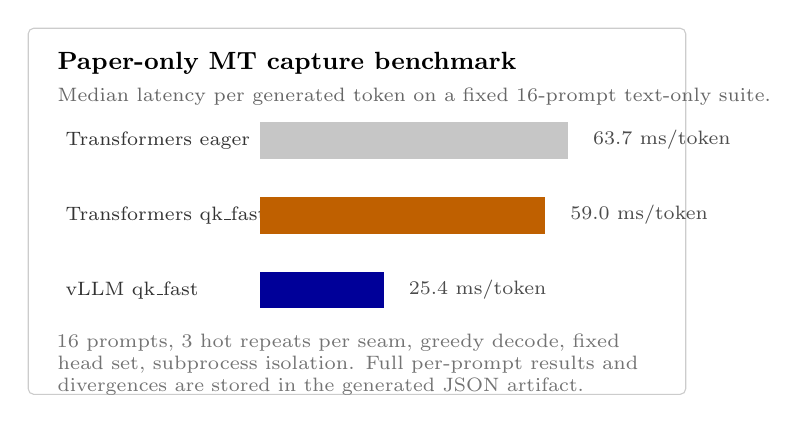
\begin{tikzpicture}[x=1cm,y=1cm, every node/.style={font=\scriptsize}]
\draw[rounded corners=2pt, fill=white, draw=black!20] (0,-0.2) rectangle (8.35,4.45);
\node[anchor=west, font=\bfseries\small] at (0.25,4.00) {Paper-only MT capture benchmark};
\node[anchor=west, text=black!60] at (0.25,3.58) {Median latency per generated token on a fixed 16-prompt text-only suite.};
\node[anchor=west, text=black!80] at (0.35,3.02) {Transformers eager};
\filldraw[fill=gray!45, draw=gray!45] (2.95,2.80) rectangle (6.85,3.25);
\node[anchor=west, text=black!70] at (7.05,3.03) {63.7 ms/token};
\node[anchor=west, text=black!80] at (0.35,2.07) {Transformers qk\_fast};
\filldraw[fill=orange!75!black, draw=orange!75!black] (2.95,1.85) rectangle (6.56,2.30);
\node[anchor=west, text=black!70] at (6.76,2.08) {59.0 ms/token};
\node[anchor=west, text=black!80] at (0.35,1.12) {vLLM qk\_fast};
\filldraw[fill=blue!60!black, draw=blue!60!black] (2.95,0.90) rectangle (4.51,1.35);
\node[anchor=west, text=black!70] at (4.71,1.13) {25.4 ms/token};
\node[anchor=west, text=black!55, align=left, text width=7.7cm] at (0.25,0.18) {16 prompts, 3 hot repeats per seam, greedy decode, fixed head set, subprocess isolation. Full per-prompt results and divergences are stored in the generated JSON artifact.};
\end{tikzpicture}
}
\caption{\textbf{Inference-time comparison of MT capture seams.} We compare a minimal Transformers eager reference, a Transformers qk-fast reference that reconstructs source rows from captured layer inputs, and the engine-native vLLM qk-fast path used by the shipped backend. The main plot reports the median latency per generated token on a fixed 16-prompt benchmark suite, with one unmeasured warmup pass and repeated hot runs per seam.}
\label{fig:mt-capture-speed}
\end{figure}


\subsection{Coordination Regimes and Compute-Aware Latency}

Our cascade loads the ASR and MT models as two separate blocking
\texttt{vllm.LLM} instances on a single GPU, which serializes every
audio chunk into an ASR decode followed by an MT decode
(Fig.~\ref{fig:coord-regimes}\,(c)). This regime is sufficient for the
IWSLT~2026 evaluation because the scoring is compute-unaware: translation
timestamps are those at which tokens become committable under the emission
policy, not those at which they materialize on the GPU. Two alternative
regimes, MT pipelined at the ASR cadence
(Fig.~\ref{fig:coord-regimes}\,(b)) and a fully asynchronous regime in
which a single MT request is relaunched on completion over the
monotonic source prefix (Fig.~\ref{fig:coord-regimes}\,(a)), would
reduce the compute-aware LongYAAL at fixed compute-unaware latency, at
the cost of a non-blocking scheduler (\texttt{AsyncLLMEngine} with
abort on stale requests). Full async additionally weakens the continuity
assumption behind fixed-cadence prefix-stability heuristics, since two
consecutive MT prompts can differ arbitrarily in length. We leave the
quantitative study of this scheduler axis to future work.

\begin{figure*}[!htbp]
\centering
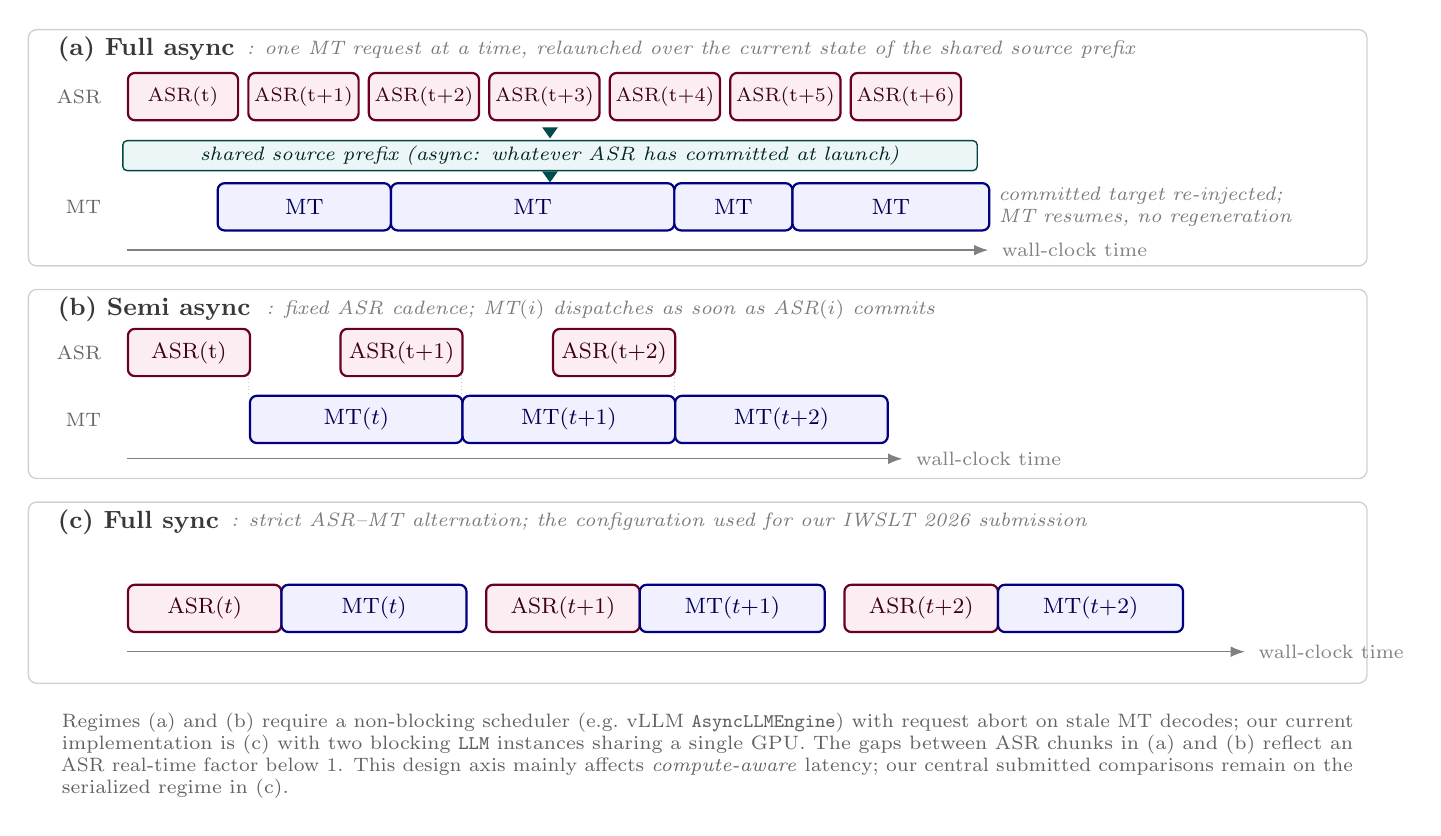
\begin{tikzpicture}[
  x=1cm, y=1cm,
  >={Latex[length=1.8mm]},
  asr/.style={
    draw=purple!55!black, rounded corners=2.5pt, line width=0.8pt,
    fill=purple!7, minimum height=0.60cm, align=center,
    font=\footnotesize, text=purple!32!black, inner sep=1.5pt,
  },
  asrsmall/.style={
    draw=purple!55!black, rounded corners=2.5pt, line width=0.8pt,
    fill=purple!7, minimum height=0.60cm, align=center,
    font=\scriptsize, text=purple!32!black, inner sep=1pt,
    minimum width=1.40cm,
  },
  mt/.style={
    draw=blue!50!black, rounded corners=2.5pt, line width=0.8pt,
    fill=blue!6, minimum height=0.60cm, align=center,
    font=\footnotesize, text=blue!32!black, inner sep=1.5pt,
  },
  buffer/.style={
    draw=teal!55!black, rounded corners=1.5pt, line width=0.5pt,
    fill=teal!7,
  },
  flowin/.style={->, draw=teal!60!black, line width=0.45pt, densely dotted},
  flowout/.style={->, draw=teal!60!black, line width=0.45pt, densely dashed},
  dispatch/.style={draw=black!22, line width=0.35pt, densely dotted},
  panel/.style={draw=black!18, rounded corners=3pt, line width=0.5pt},
  timeaxis/.style={->, draw=black!50, line width=0.5pt},
  panelhdr/.style={font=\small\bfseries, text=black!78, anchor=west},
  panelsub/.style={font=\scriptsize\itshape, text=black!52, anchor=west},
  lanelabel/.style={font=\scriptsize, text=black!60, anchor=east},
  tick/.style={font=\scriptsize, text=black!50, anchor=west},
  buflabel/.style={font=\scriptsize\itshape, text=teal!28!black, anchor=west},
]

  %% ==========================================================
  %% Panel (a): Full async
  %% ==========================================================
  \draw[panel] (0.00, 9.10) rectangle (17.00, 12.10);
  \node[panelhdr] at (0.25, 11.85) {(a) Full async};
  \node[panelsub] at (2.60, 11.85)
    {\,: one MT request at a time, relaunched over the current state of the shared source prefix};

  % ASR lane: 7 chunks, fixed cadence, with gaps reflecting RTF_ASR < 1
  \node[lanelabel] at (1.05, 11.25) {ASR};
  \foreach \i/\lbl in {0/{$t$}, 1/{$t{+}1$}, 2/{$t{+}2$}, 3/{$t{+}3$}, 4/{$t{+}4$}, 5/{$t{+}5$}, 6/{$t{+}6$}} {
    \node[asrsmall, anchor=west]
      at ({1.25 + \i*1.53}, 11.25) {ASR$(\lbl)$};
  }

  % Buffer strip between lanes
  \draw[buffer] (1.20, 10.31) rectangle (12.05, 10.69);
  \pgfmathsetmacro{\bufCx}{(1.20 + 12.05)/2}
  \node[buflabel, align=center, text width=10.40cm, anchor=center]
    at (\bufCx, 10.50)
    {shared source prefix \textmd{(async: whatever ASR has committed at launch)}};

  % Flow hints: ASR appends into the shared prefix, then MT relaunches from it
  % Both markers are centered horizontally on the shared source prefix block
  \fill[teal!60!black] (\bufCx, 10.72) -- ({\bufCx - 0.10}, 10.86) -- ({\bufCx + 0.10}, 10.86) -- cycle;
  \fill[teal!60!black] (\bufCx, 10.16) -- ({\bufCx - 0.10}, 10.30) -- ({\bufCx + 0.10}, 10.30) -- cycle;

  % MT lane: 4 variable-length decodes (relaunched on completion); widths are
  % non-monotonic: a long MT call "consumes" many ASR chunks, so the next call
  % has less new source to translate and is shorter.
  \node[lanelabel] at (1.05, 9.85) {MT};
  \node[mt, minimum width=2.20cm, anchor=west] at (2.39, 9.85) {MT};
  \node[mt, minimum width=3.60cm, anchor=west] at (4.59, 9.85) {MT};
  \node[mt, minimum width=1.50cm, anchor=west] at (8.19, 9.85) {MT};
  \node[mt, minimum width=2.50cm, anchor=west] at (9.69, 9.85) {MT};
  % Note: MT resumes from the previously committed target, not from scratch.
  % Forced line break keeps the note within 2 lines so it does not overflow
  % the panel or the MT lane vertical band.
  \node[font=\scriptsize\itshape, text=black!52, anchor=west,
        text width=4.40cm, align=left, inner sep=1pt]
    at (12.30, 9.85)
    {committed target re-injected;\\MT resumes, no regeneration};

  % Time axis
  \draw[timeaxis] (1.25, 9.30) -- (12.19, 9.30);
  \node[tick] at (12.24, 9.30) {wall-clock time};

  %% ==========================================================
  %% Panel (b): Semi async
  %% ==========================================================
  \draw[panel] (0.00, 6.40) rectangle (17.00, 8.80);
  \node[panelhdr] at (0.25, 8.55) {(b) Semi async};
  \node[panelsub] at (2.85, 8.55)
    {\,: fixed ASR cadence; MT$(i)$ dispatches as soon as ASR$(i)$ commits};

  % ASR lane: gaps between chunks (RTF_ASR < 1)
  \node[lanelabel] at (1.05, 8.00) {ASR};
  \foreach \i/\lbl in {0/{$t$}, 1/{$t{+}1$}, 2/{$t{+}2$}} {
    \node[asr, minimum width=1.55cm, anchor=west]
      at ({1.25 + \i*2.70}, 8.00) {ASR$(\lbl)$};
  }

  % MT lane: pipelined, GPU-constrained to one at a time
  \node[lanelabel] at (1.05, 7.15) {MT};
  \foreach \x in {2.80, 5.50, 8.20} {
    \draw[dispatch] (\x, 7.72) -- (\x, 7.47);
  }
  \node[mt, minimum width=2.70cm, anchor=west] at (2.80, 7.15) {MT$(t)$};
  \node[mt, minimum width=2.70cm, anchor=west] at (5.50, 7.15) {MT$(t{+}1)$};
  \node[mt, minimum width=2.70cm, anchor=west] at (8.20, 7.15) {MT$(t{+}2)$};

  % Time axis
  \draw[timeaxis] (1.25, 6.65) -- (11.10, 6.65);
  \node[tick] at (11.15, 6.65) {wall-clock time};

  %% ==========================================================
  %% Panel (c): Full sync
  %% ==========================================================
  \draw[panel] (0.00, 3.80) rectangle (17.00, 6.10);
  \node[panelhdr] at (0.25, 5.85) {(c) Full sync};
  \node[panelsub] at (2.40, 5.85)
    {\,: strict ASR--MT alternation; the configuration used for our IWSLT~2026 submission};

  % Single alternating row; ASR(i) and MT(i) are glued together (tight pair)
  \node[asr, minimum width=1.95cm, anchor=west] at (1.25, 4.75) {ASR$(t)$};
  \node[mt,  minimum width=2.35cm, anchor=west] at (3.20, 4.75) {MT$(t)$};
  \node[asr, minimum width=1.95cm, anchor=west] at (5.80, 4.75) {ASR$(t{+}1)$};
  \node[mt,  minimum width=2.35cm, anchor=west] at (7.75, 4.75) {MT$(t{+}1)$};
  \node[asr, minimum width=1.95cm, anchor=west] at (10.35, 4.75) {ASR$(t{+}2)$};
  \node[mt,  minimum width=2.35cm, anchor=west] at (12.30, 4.75) {MT$(t{+}2)$};

  % Time axis
  \draw[timeaxis] (1.25, 4.20) -- (15.45, 4.20);
  \node[tick] at (15.50, 4.20) {wall-clock time};

  %% ==========================================================
  %% Bottom note
  %% ==========================================================
  \node[anchor=north west, font=\scriptsize, text=black!62, align=justify, text width=16.4cm]
    at (0.30, 3.55)
    {Regimes (a) and (b) require a non-blocking scheduler (e.g.\ vLLM \texttt{AsyncLLMEngine}) with request abort on stale MT decodes; our current implementation is (c) with two blocking \texttt{LLM} instances sharing a single GPU. The gaps between ASR chunks in (a) and (b) reflect an ASR real-time factor below~1. This design axis mainly affects \emph{compute-aware} latency; our central submitted comparisons remain on the serialized regime in (c).};

\end{tikzpicture}
\caption{\label{fig:coord-regimes}%
Three coordination regimes for ASR and MT sharing one GPU. The submitted system uses the strict ASR--MT alternation in~(c).}
\end{figure*}


\section{Conclusion}
\label{sec:conclusion}

The retained IWSLT 2026 system is a Qwen3 forced ASR + Gemma-4 MT cascade, and
its key technical ingredient is an engine-native realization of AlignAtt for
decoder-only MT under compiled inference. Deterministic prompt layout, offline
head selection, selective \emph{qk-fast} replay, and compile-safe query/key
capture make the MT policy usable without leaving the deployed runtime. On the
dev set, this yields a low-latency operating point near 2\,s CU-LongYAAL and a
high-latency regime that is roughly 1.5\,s slower but clearly stronger in
BLEU and XCOMET-XL. The main limitations are that evaluation is single-GPU and
dev-set only, and that the contribution is on the MT observer rather than on
speech modeling itself.

\bibliography{references}

\appendix

\section{Formal Cascade Definition}
\label{sec:cascade}

\paragraph{Streaming input and alignment backend.}
The system is invoked on a monotone sequence of timestamps
$t_1 < t_2 < \cdots$ with $t_{k+1} - t_k = \Delta_{\mathrm{chunk}}$.
At each $t_k$, the ASR/alignment backend returns a live transcript prefix
$\mathbf{s}^{(k)} = (s^{(k)}_1, \ldots, s^{(k)}_{N_k})$ together with per-word
end times $\theta^{(k)}_i \in \mathbb{R}_{\geq 0}$, $i=1,\ldots,N_k$.
Throughout this appendix, bold symbols denote ordered token sequences and
calligraphic symbols denote index sets; in particular
$\mathcal{S}^{(k)} := \{1,\ldots,N_k\}$ is the local index set of the live
source prefix at step $k$.

\paragraph{Source accessibility frontier.}
Given an inaccessibility margin $\tau_{\mathrm{in}} \ge 0$, the accessible
source index set at time $t_k$ is
\begin{equation}
  \mathcal{S}^{(k)}_{\mathrm{acc}}
  = \Bigl\{\, i \in \mathcal{S}^{(k)}
     \;\Bigm|\; \theta^{(k)}_i \le t_k - \tau_{\mathrm{in}} \,\Bigr\},
  \label{eq:frontier}
\end{equation}
with $N^{(k)}_{\mathrm{acc}} = |\mathcal{S}^{(k)}_{\mathrm{acc}}|$. On the
final chunk we set $N^{(k)}_{\mathrm{acc}} = N_k$. The inaccessible complement
is $\mathcal{S}^{(k)}_{\mathrm{inacc}} =
\mathcal{S}^{(k)} \setminus \mathcal{S}^{(k)}_{\mathrm{acc}}$.

\paragraph{Translation backend.}
The MT backend maps the live source $\mathbf{s}^{(k)}$ and the already
accepted target prefix $\mathbf{y}_{1:m_k}$ to a draft
$\widetilde{\mathbf{y}}^{(k)} =
(\widetilde{y}^{(k)}_1, \ldots, \widetilde{y}^{(k)}_{L_k})$ of at most
$L_{\mathrm{draft}}$ new target tokens.

\paragraph{Acceptance and emission.}
An AlignAtt policy $\Pi$ turns the draft into an accepted suffix
$\mathbf{a}^{(k)}$ of length $\ell_k \in \{0,1,\ldots,L_k\}$:
\begin{equation}
  \mathbf{a}^{(k)} = \Pi\!\left(
    \widetilde{\mathbf{y}}^{(k)},\, \mathcal{S}^{(k)}_{\mathrm{acc}}
  \right),
  \label{eq:accept-prefix}
\end{equation}
so $\mathbf{a}^{(k)} =
(\widetilde{y}^{(k)}_1, \ldots, \widetilde{y}^{(k)}_{\ell_k})$ is the retained
draft prefix. The accepted target prefix then extends monotonically:
\begin{equation}
  \mathbf{y}_{1:m_{k+1}} =
  \mathbf{y}_{1:m_k} \,\Vert\, \mathbf{a}^{(k)},
  \label{eq:monotone}
\end{equation}
with $m_{k+1} = m_k + \ell_k$. Already emitted target tokens are never
retracted.

Figure~\ref{fig:system} gives the submission-specific operational view; this
appendix keeps only the role-agnostic notation needed for the later
derivations.

\paragraph{Latency functional.}
Let $\tau^{\mathrm{emit}}_j$ denote the wall-clock emission time of target
token $y_j$ and $\tau^{\mathrm{src}}_j$ the end time of the source word
responsible for it. The main latency metric in this paper is the
compute-unaware LongYAAL latency:
\begin{equation}
  \mathrm{LongYAAL}_{\mathrm{CU}}(\mathbf{y})
  = \frac{1}{|\mathbf{y}|} \sum_{j=1}^{|\mathbf{y}|}
  \bigl(\tau^{\mathrm{emit}}_j - \tau^{\mathrm{src}}_j\bigr)_+,
  \label{eq:lya-cu}
\end{equation}
with $(u)_+ = \max(u,0)$ \citep{longyaal25}.

\section{Additional Decoder-Only AlignAtt Details}
\label{sec:appendix-alignatt}
\label{sec:alignatt-llm}

\paragraph{From encoder--decoder AlignAtt to decoder-only MT.}
In its original formulation, AlignAtt exploits decoder cross-attention in an
encoder--decoder speech translation model \citep{alignatt23}: each decoder row
is normalized over source positions only, so source provenance is built into
the architecture. In a decoder-only LLM there is no cross-attention. A single
causal token stream mixes instructions, source, accepted target history, and
the current draft, and each row of self-attention is normalized over all prompt
positions. Relative to the encoder--decoder setting, the attention row no
longer distinguishes source from non-source by construction, and no head is
architecturally reserved for source alignment.

\paragraph{Prompt-induced source span.}
We therefore recover a source-target distinction through prompt layout rather
than architecture. At MT step $k$, the prompt is assembled as
\begin{equation}
  \mathbf{p}^{(k)} = \bigl[\,
  \mathbf{p}^{\mathrm{sys}}
  \Vert \mathbf{s}^{(k)}
  \Vert \mathbf{p}^{\mathrm{instr}}, \mathbf{y}_{1:m_k}
  \Vert \widetilde{\mathbf{y}}^{(k)} \,\bigr],
  \label{eq:layout}
\end{equation}
where $\mathbf{s}^{(k)}$ is the live transcript prefix,
$\mathbf{y}_{1:m_k}$ the accepted target prefix, and
$\widetilde{\mathbf{y}}^{(k)}$ the drafted continuation. Let
$\phi^{(k)} : \mathcal{S}^{(k)} \hookrightarrow \{1,\ldots,n\}$ map local
source indices to absolute prompt positions.

\paragraph{Virtual source-restricted attention rows.}
The object relevant to alignment is then the source slice of
self-attention. For draft position $t$ and source index $s$, we read
\begin{equation}
  \mathbf{A}^{(\ell,h)}_{\mathrm{src}}(t,s)
  := \mathbf{A}^{(\ell,h)}_{t,\,\phi^{(k)}(s)},
  \label{eq:virtual-xattn}
\end{equation}
at layer $\ell$ and head $h$. Unlike encoder--decoder cross-attention,
$\sum_{s \in \mathcal{S}^{(k)}} \mathbf{A}^{(\ell,h)}_{\mathrm{src}}(t,s) < 1$
in general because the row is normalized over the entire prompt. Residual mass
on non-source prompt positions and on the draft is therefore structural, not an
implementation artifact.

\paragraph{What stays the same and what changes.}
The online decision rule still follows the original AlignAtt spirit: accept the
longest draft prefix whose source-side alignment signal remains inside the
accessible frontier. What changes is the substrate on which that signal is
observed. In the decoder-only case, we carve source-restricted rows out of the
full-prompt self-attention tensor and keep track of the residual mass on the
accepted target prefix, the rest of the prompt, and the speculative suffix.

\paragraph{Alignment heads.}
Not all self-attention heads carry translation alignment signal. We assume the
existence of a small head subset
$\mathcal{H} \subset \{1,\ldots,L\} \times \{1,\ldots,H\}$,
$|\mathcal{H}| \ll LH$, such that the head-averaged source row approximates
gold source-to-target alignments on a held-out calibration set
$\mathcal{G} = \{(\mathbf{s}^{(i)}, \mathbf{y}^{(i)}, \mathbf{a}^{(i)})\}_i$,
where $\mathbf{a}^{(i)}$ is a forced word-level alignment. This sparsity
assumption is consistent with recent evidence that multilingual LLMs contain a
small set of translation-specific alignment heads \citep{tokenheads26}.

\paragraph{Offline head selection.}
For one head $(\ell,h)$, define the argmax alignment
\begin{equation}
  \hat{a}^{(\ell,h)}_t(\mathbf{s}, \mathbf{y})
  = \arg\max_s \mathbf{A}^{(\ell,h)}_{t,\phi(s)},
  \label{eq:head-argmax}
\end{equation}
and its token-level alignment accuracy
\begin{equation}
  \begin{aligned}
    \mathrm{Acc}_{\mathrm{align}}(\ell,h)
    &=
    \frac{1}{|\mathcal{G}|}
    \sum_i \frac{1}{|\mathbf{y}^{(i)}|} \\
    &\qquad \cdot
    \sum_{t=1}^{|\mathbf{y}^{(i)}|}
    \mathbf{1}\!\bigl[\hat{a}^{(\ell,h)}_t = \mathbf{a}^{(i)}_t\bigr].
  \end{aligned}
  \label{eq:align-acc}
\end{equation}
We then select
$\mathcal{H} = \operatorname*{top-}k_{(\ell,h)}
\mathrm{Acc}_{\mathrm{align}}(\ell,h)$ with $k=8$.

\noindent Before testing these head sets end-to-end in
Section~\ref{sec:head-filtering}, we first score them on held-out word-aligned
MT examples under the same prompt layout. Table~\ref{tab:mt-head-filtering}
shows that the retained top-8 heads preserve a markedly stronger alignment
signal than uniform all-head averaging even when the all-head baseline is made
maximally charitable by restricting its argmax to the source-prompt zone
before scoring.

\begin{table}[t]
\centering
\small
\resizebox{\columnwidth}{!}{%
\begin{tabular}{l r r r r}
\toprule
Pair & Top-8 TS & All-336 TS & Gain & Aligned tokens \\
\midrule
EN$\to$DE & 90.40 & 68.49 & \textbf{+21.91} & 11,209 \\
EN$\to$ZH & 93.48 & 65.79 & \textbf{+27.70} & 7,582 \\
EN$\to$IT & 91.90 & 67.42 & \textbf{+24.49} & 12,056 \\
\bottomrule
\end{tabular}
}
\caption{\textbf{MT head-set filtering ablation on held-out word-aligned dev examples.} To make the all-head baseline maximally charitable, we average the candidate head set first and then restrict the argmax to the source-prompt token zone before scoring against gold aligned source tokens. Scores are reported in points ($100\times\mathrm{TS}$). Even under this source-only argmax, the per-direction retained top-8 heads still preserve a markedly stronger alignment signal than uniform all-head averaging.}
\label{tab:mt-head-filtering}
\end{table}


\begin{figure*}[t]
\centering
\resizebox{\linewidth}{!}{%
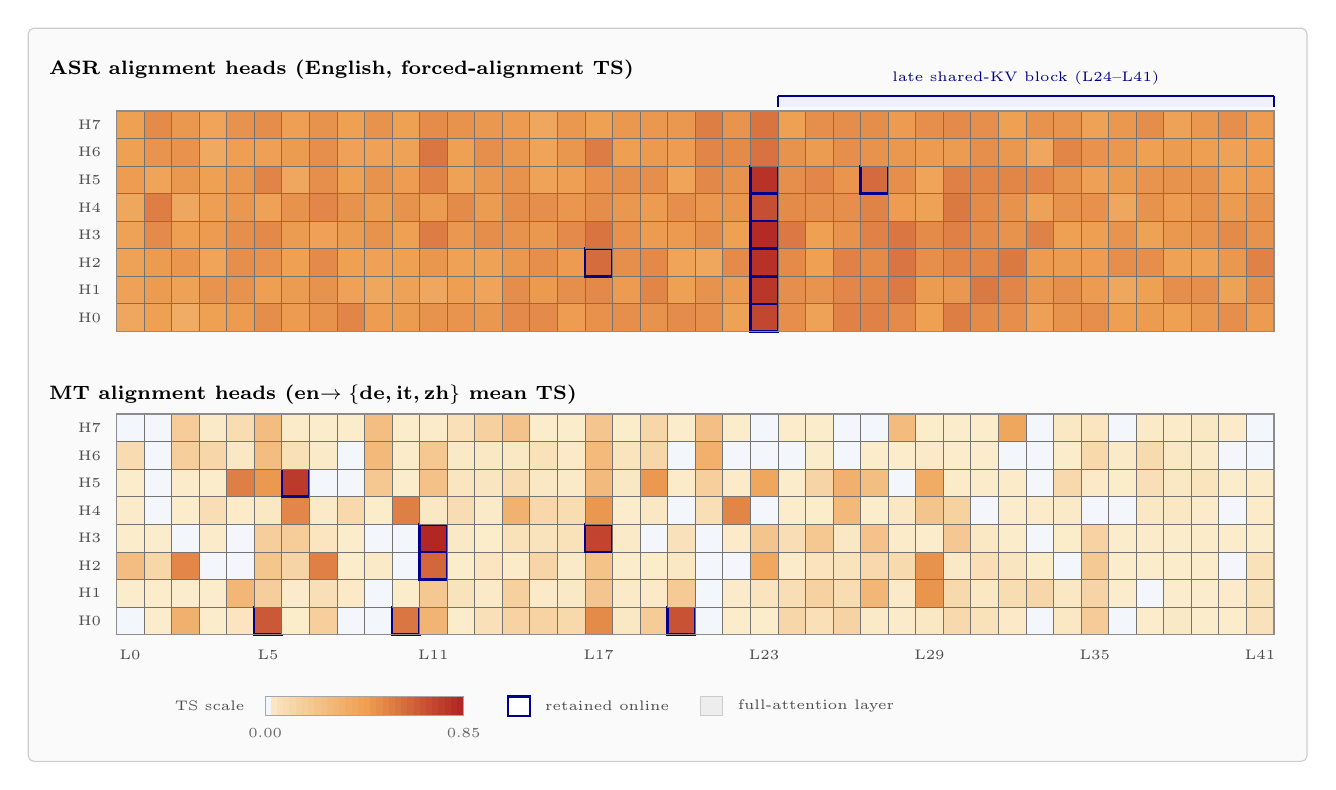
\begin{tikzpicture}[x=0.35cm,y=0.35cm, every node/.style={font=\scriptsize}]
\draw[rounded corners=2pt, fill=black!2, draw=black!20] (-3.2,-4.60) rectangle (43.2,22.00);
\node[anchor=west, font=\bfseries\scriptsize] at (-2.8,20.50) {ASR alignment heads (English, forced-alignment TS)};
\fill[black!7] (16.98,10.98) rectangle (18.02,19.02);
\fill[black!7] (34.98,10.98) rectangle (36.02,19.02);
\fill[black!7] (4.98,10.98) rectangle (6.02,19.02);
\fill[black!7] (22.98,10.98) rectangle (24.02,19.02);
\fill[black!7] (40.98,10.98) rectangle (42.02,19.02);
\fill[black!7] (10.98,10.98) rectangle (12.02,19.02);
\fill[black!7] (28.98,10.98) rectangle (30.02,19.02);
\fill[blue!6] (24.00,19.15) rectangle (42.00,19.55);
\draw[blue!55!black, line width=0.7pt] (24.00,19.15) -- (24.00,19.55);
\draw[blue!55!black, line width=0.7pt] (42.00,19.15) -- (42.00,19.55);
\draw[blue!55!black, line width=0.7pt] (24.00,19.55) -- (42.00,19.55);
\node[anchor=south, font=\tiny, text=blue!55!black] at (33.00,19.60) {late shared-KV block (L24--L41)};
\filldraw[fill={rgb,255:red,239; green,166; blue,94}, draw=black!55, line width=0.25pt] (0.00,11.00) rectangle (1.00,12.00);
\filldraw[fill={rgb,255:red,239; green,162; blue,87}, draw=black!55, line width=0.25pt] (0.00,12.00) rectangle (1.00,13.00);
\filldraw[fill={rgb,255:red,238; green,162; blue,87}, draw=black!55, line width=0.25pt] (0.00,13.00) rectangle (1.00,14.00);
\filldraw[fill={rgb,255:red,238; green,162; blue,87}, draw=black!55, line width=0.25pt] (0.00,14.00) rectangle (1.00,15.00);
\filldraw[fill={rgb,255:red,239; green,167; blue,94}, draw=black!55, line width=0.25pt] (0.00,15.00) rectangle (1.00,16.00);
\filldraw[fill={rgb,255:red,237; green,156; blue,81}, draw=black!55, line width=0.25pt] (0.00,16.00) rectangle (1.00,17.00);
\filldraw[fill={rgb,255:red,238; green,160; blue,83}, draw=black!55, line width=0.25pt] (0.00,17.00) rectangle (1.00,18.00);
\filldraw[fill={rgb,255:red,238; green,160; blue,83}, draw=black!55, line width=0.25pt] (0.00,18.00) rectangle (1.00,19.00);
\filldraw[fill={rgb,255:red,238; green,160; blue,83}, draw=black!55, line width=0.25pt] (1.00,11.00) rectangle (2.00,12.00);
\filldraw[fill={rgb,255:red,236; green,156; blue,81}, draw=black!55, line width=0.25pt] (1.00,12.00) rectangle (2.00,13.00);
\filldraw[fill={rgb,255:red,236; green,156; blue,81}, draw=black!55, line width=0.25pt] (1.00,13.00) rectangle (2.00,14.00);
\filldraw[fill={rgb,255:red,228; green,138; blue,74}, draw=black!55, line width=0.25pt] (1.00,14.00) rectangle (2.00,15.00);
\filldraw[fill={rgb,255:red,222; green,126; blue,69}, draw=black!55, line width=0.25pt] (1.00,15.00) rectangle (2.00,16.00);
\filldraw[fill={rgb,255:red,239; green,164; blue,90}, draw=black!55, line width=0.25pt] (1.00,16.00) rectangle (2.00,17.00);
\filldraw[fill={rgb,255:red,232; green,148; blue,78}, draw=black!55, line width=0.25pt] (1.00,17.00) rectangle (2.00,18.00);
\filldraw[fill={rgb,255:red,228; green,139; blue,74}, draw=black!55, line width=0.25pt] (1.00,18.00) rectangle (2.00,19.00);
\filldraw[fill={rgb,255:red,240; green,171; blue,101}, draw=black!55, line width=0.25pt] (2.00,11.00) rectangle (3.00,12.00);
\filldraw[fill={rgb,255:red,238; green,162; blue,86}, draw=black!55, line width=0.25pt] (2.00,12.00) rectangle (3.00,13.00);
\filldraw[fill={rgb,255:red,234; green,150; blue,79}, draw=black!55, line width=0.25pt] (2.00,13.00) rectangle (3.00,14.00);
\filldraw[fill={rgb,255:red,238; green,159; blue,82}, draw=black!55, line width=0.25pt] (2.00,14.00) rectangle (3.00,15.00);
\filldraw[fill={rgb,255:red,239; green,166; blue,94}, draw=black!55, line width=0.25pt] (2.00,15.00) rectangle (3.00,16.00);
\filldraw[fill={rgb,255:red,234; green,151; blue,79}, draw=black!55, line width=0.25pt] (2.00,16.00) rectangle (3.00,17.00);
\filldraw[fill={rgb,255:red,232; green,146; blue,77}, draw=black!55, line width=0.25pt] (2.00,17.00) rectangle (3.00,18.00);
\filldraw[fill={rgb,255:red,234; green,151; blue,79}, draw=black!55, line width=0.25pt] (2.00,18.00) rectangle (3.00,19.00);
\filldraw[fill={rgb,255:red,238; green,160; blue,83}, draw=black!55, line width=0.25pt] (3.00,11.00) rectangle (4.00,12.00);
\filldraw[fill={rgb,255:red,232; green,148; blue,78}, draw=black!55, line width=0.25pt] (3.00,12.00) rectangle (4.00,13.00);
\filldraw[fill={rgb,255:red,239; green,164; blue,90}, draw=black!55, line width=0.25pt] (3.00,13.00) rectangle (4.00,14.00);
\filldraw[fill={rgb,255:red,236; green,155; blue,81}, draw=black!55, line width=0.25pt] (3.00,14.00) rectangle (4.00,15.00);
\filldraw[fill={rgb,255:red,238; green,159; blue,83}, draw=black!55, line width=0.25pt] (3.00,15.00) rectangle (4.00,16.00);
\filldraw[fill={rgb,255:red,238; green,160; blue,83}, draw=black!55, line width=0.25pt] (3.00,16.00) rectangle (4.00,17.00);
\filldraw[fill={rgb,255:red,240; green,169; blue,97}, draw=black!55, line width=0.25pt] (3.00,17.00) rectangle (4.00,18.00);
\filldraw[fill={rgb,255:red,239; green,164; blue,90}, draw=black!55, line width=0.25pt] (3.00,18.00) rectangle (4.00,19.00);
\filldraw[fill={rgb,255:red,236; green,156; blue,81}, draw=black!55, line width=0.25pt] (4.00,11.00) rectangle (5.00,12.00);
\filldraw[fill={rgb,255:red,232; green,147; blue,77}, draw=black!55, line width=0.25pt] (4.00,12.00) rectangle (5.00,13.00);
\filldraw[fill={rgb,255:red,230; green,143; blue,76}, draw=black!55, line width=0.25pt] (4.00,13.00) rectangle (5.00,14.00);
\filldraw[fill={rgb,255:red,230; green,143; blue,76}, draw=black!55, line width=0.25pt] (4.00,14.00) rectangle (5.00,15.00);
\filldraw[fill={rgb,255:red,234; green,151; blue,79}, draw=black!55, line width=0.25pt] (4.00,15.00) rectangle (5.00,16.00);
\filldraw[fill={rgb,255:red,234; green,151; blue,79}, draw=black!55, line width=0.25pt] (4.00,16.00) rectangle (5.00,17.00);
\filldraw[fill={rgb,255:red,238; green,159; blue,83}, draw=black!55, line width=0.25pt] (4.00,17.00) rectangle (5.00,18.00);
\filldraw[fill={rgb,255:red,232; green,147; blue,77}, draw=black!55, line width=0.25pt] (4.00,18.00) rectangle (5.00,19.00);
\filldraw[fill={rgb,255:red,229; green,142; blue,75}, draw=black!55, line width=0.25pt] (5.00,11.00) rectangle (6.00,12.00);
\filldraw[fill={rgb,255:red,238; green,159; blue,82}, draw=black!55, line width=0.25pt] (5.00,12.00) rectangle (6.00,13.00);
\filldraw[fill={rgb,255:red,231; green,146; blue,77}, draw=black!55, line width=0.25pt] (5.00,13.00) rectangle (6.00,14.00);
\filldraw[fill={rgb,255:red,227; green,137; blue,73}, draw=black!55, line width=0.25pt] (5.00,14.00) rectangle (6.00,15.00);
\filldraw[fill={rgb,255:red,239; green,162; blue,87}, draw=black!55, line width=0.25pt] (5.00,15.00) rectangle (6.00,16.00);
\filldraw[fill={rgb,255:red,225; green,132; blue,72}, draw=black!55, line width=0.25pt] (5.00,16.00) rectangle (6.00,17.00);
\filldraw[fill={rgb,255:red,238; green,161; blue,86}, draw=black!55, line width=0.25pt] (5.00,17.00) rectangle (6.00,18.00);
\filldraw[fill={rgb,255:red,229; green,141; blue,75}, draw=black!55, line width=0.25pt] (5.00,18.00) rectangle (6.00,19.00);
\filldraw[fill={rgb,255:red,236; green,155; blue,80}, draw=black!55, line width=0.25pt] (6.00,11.00) rectangle (7.00,12.00);
\filldraw[fill={rgb,255:red,236; green,156; blue,81}, draw=black!55, line width=0.25pt] (6.00,12.00) rectangle (7.00,13.00);
\filldraw[fill={rgb,255:red,238; green,160; blue,83}, draw=black!55, line width=0.25pt] (6.00,13.00) rectangle (7.00,14.00);
\filldraw[fill={rgb,255:red,236; green,156; blue,81}, draw=black!55, line width=0.25pt] (6.00,14.00) rectangle (7.00,15.00);
\filldraw[fill={rgb,255:red,232; green,147; blue,77}, draw=black!55, line width=0.25pt] (6.00,15.00) rectangle (7.00,16.00);
\filldraw[fill={rgb,255:red,239; green,166; blue,94}, draw=black!55, line width=0.25pt] (6.00,16.00) rectangle (7.00,17.00);
\filldraw[fill={rgb,255:red,236; green,156; blue,81}, draw=black!55, line width=0.25pt] (6.00,17.00) rectangle (7.00,18.00);
\filldraw[fill={rgb,255:red,238; green,159; blue,83}, draw=black!55, line width=0.25pt] (6.00,18.00) rectangle (7.00,19.00);
\filldraw[fill={rgb,255:red,232; green,147; blue,77}, draw=black!55, line width=0.25pt] (7.00,11.00) rectangle (8.00,12.00);
\filldraw[fill={rgb,255:red,232; green,147; blue,77}, draw=black!55, line width=0.25pt] (7.00,12.00) rectangle (8.00,13.00);
\filldraw[fill={rgb,255:red,228; green,138; blue,74}, draw=black!55, line width=0.25pt] (7.00,13.00) rectangle (8.00,14.00);
\filldraw[fill={rgb,255:red,239; green,162; blue,87}, draw=black!55, line width=0.25pt] (7.00,14.00) rectangle (8.00,15.00);
\filldraw[fill={rgb,255:red,226; green,135; blue,73}, draw=black!55, line width=0.25pt] (7.00,15.00) rectangle (8.00,16.00);
\filldraw[fill={rgb,255:red,230; green,143; blue,76}, draw=black!55, line width=0.25pt] (7.00,16.00) rectangle (8.00,17.00);
\filldraw[fill={rgb,255:red,230; green,143; blue,76}, draw=black!55, line width=0.25pt] (7.00,17.00) rectangle (8.00,18.00);
\filldraw[fill={rgb,255:red,232; green,147; blue,77}, draw=black!55, line width=0.25pt] (7.00,18.00) rectangle (8.00,19.00);
\filldraw[fill={rgb,255:red,225; green,134; blue,72}, draw=black!55, line width=0.25pt] (8.00,11.00) rectangle (9.00,12.00);
\filldraw[fill={rgb,255:red,239; green,162; blue,87}, draw=black!55, line width=0.25pt] (8.00,12.00) rectangle (9.00,13.00);
\filldraw[fill={rgb,255:red,238; green,160; blue,83}, draw=black!55, line width=0.25pt] (8.00,13.00) rectangle (9.00,14.00);
\filldraw[fill={rgb,255:red,236; green,156; blue,81}, draw=black!55, line width=0.25pt] (8.00,14.00) rectangle (9.00,15.00);
\filldraw[fill={rgb,255:red,232; green,147; blue,77}, draw=black!55, line width=0.25pt] (8.00,15.00) rectangle (9.00,16.00);
\filldraw[fill={rgb,255:red,238; green,160; blue,83}, draw=black!55, line width=0.25pt] (8.00,16.00) rectangle (9.00,17.00);
\filldraw[fill={rgb,255:red,239; green,162; blue,87}, draw=black!55, line width=0.25pt] (8.00,17.00) rectangle (9.00,18.00);
\filldraw[fill={rgb,255:red,238; green,160; blue,83}, draw=black!55, line width=0.25pt] (8.00,18.00) rectangle (9.00,19.00);
\filldraw[fill={rgb,255:red,237; green,156; blue,81}, draw=black!55, line width=0.25pt] (9.00,11.00) rectangle (10.00,12.00);
\filldraw[fill={rgb,255:red,239; green,167; blue,94}, draw=black!55, line width=0.25pt] (9.00,12.00) rectangle (10.00,13.00);
\filldraw[fill={rgb,255:red,239; green,162; blue,87}, draw=black!55, line width=0.25pt] (9.00,13.00) rectangle (10.00,14.00);
\filldraw[fill={rgb,255:red,232; green,147; blue,77}, draw=black!55, line width=0.25pt] (9.00,14.00) rectangle (10.00,15.00);
\filldraw[fill={rgb,255:red,236; green,156; blue,81}, draw=black!55, line width=0.25pt] (9.00,15.00) rectangle (10.00,16.00);
\filldraw[fill={rgb,255:red,232; green,147; blue,77}, draw=black!55, line width=0.25pt] (9.00,16.00) rectangle (10.00,17.00);
\filldraw[fill={rgb,255:red,239; green,162; blue,87}, draw=black!55, line width=0.25pt] (9.00,17.00) rectangle (10.00,18.00);
\filldraw[fill={rgb,255:red,232; green,147; blue,77}, draw=black!55, line width=0.25pt] (9.00,18.00) rectangle (10.00,19.00);
\filldraw[fill={rgb,255:red,236; green,156; blue,81}, draw=black!55, line width=0.25pt] (10.00,11.00) rectangle (11.00,12.00);
\filldraw[fill={rgb,255:red,238; green,162; blue,87}, draw=black!55, line width=0.25pt] (10.00,12.00) rectangle (11.00,13.00);
\filldraw[fill={rgb,255:red,238; green,160; blue,83}, draw=black!55, line width=0.25pt] (10.00,13.00) rectangle (11.00,14.00);
\filldraw[fill={rgb,255:red,238; green,160; blue,83}, draw=black!55, line width=0.25pt] (10.00,14.00) rectangle (11.00,15.00);
\filldraw[fill={rgb,255:red,232; green,147; blue,77}, draw=black!55, line width=0.25pt] (10.00,15.00) rectangle (11.00,16.00);
\filldraw[fill={rgb,255:red,237; green,156; blue,81}, draw=black!55, line width=0.25pt] (10.00,16.00) rectangle (11.00,17.00);
\filldraw[fill={rgb,255:red,238; green,162; blue,87}, draw=black!55, line width=0.25pt] (10.00,17.00) rectangle (11.00,18.00);
\filldraw[fill={rgb,255:red,238; green,160; blue,83}, draw=black!55, line width=0.25pt] (10.00,18.00) rectangle (11.00,19.00);
\filldraw[fill={rgb,255:red,231; green,146; blue,77}, draw=black!55, line width=0.25pt] (11.00,11.00) rectangle (12.00,12.00);
\filldraw[fill={rgb,255:red,239; green,167; blue,95}, draw=black!55, line width=0.25pt] (11.00,12.00) rectangle (12.00,13.00);
\filldraw[fill={rgb,255:red,233; green,150; blue,78}, draw=black!55, line width=0.25pt] (11.00,13.00) rectangle (12.00,14.00);
\filldraw[fill={rgb,255:red,221; green,125; blue,69}, draw=black!55, line width=0.25pt] (11.00,14.00) rectangle (12.00,15.00);
\filldraw[fill={rgb,255:red,236; green,156; blue,81}, draw=black!55, line width=0.25pt] (11.00,15.00) rectangle (12.00,16.00);
\filldraw[fill={rgb,255:red,224; green,131; blue,71}, draw=black!55, line width=0.25pt] (11.00,16.00) rectangle (12.00,17.00);
\filldraw[fill={rgb,255:red,218; green,118; blue,66}, draw=black!55, line width=0.25pt] (11.00,17.00) rectangle (12.00,18.00);
\filldraw[fill={rgb,255:red,229; green,140; blue,75}, draw=black!55, line width=0.25pt] (11.00,18.00) rectangle (12.00,19.00);
\filldraw[fill={rgb,255:red,232; green,147; blue,78}, draw=black!55, line width=0.25pt] (12.00,11.00) rectangle (13.00,12.00);
\filldraw[fill={rgb,255:red,238; green,159; blue,82}, draw=black!55, line width=0.25pt] (12.00,12.00) rectangle (13.00,13.00);
\filldraw[fill={rgb,255:red,238; green,162; blue,86}, draw=black!55, line width=0.25pt] (12.00,13.00) rectangle (13.00,14.00);
\filldraw[fill={rgb,255:red,234; green,151; blue,79}, draw=black!55, line width=0.25pt] (12.00,14.00) rectangle (13.00,15.00);
\filldraw[fill={rgb,255:red,228; green,139; blue,74}, draw=black!55, line width=0.25pt] (12.00,15.00) rectangle (13.00,16.00);
\filldraw[fill={rgb,255:red,238; green,162; blue,86}, draw=black!55, line width=0.25pt] (12.00,16.00) rectangle (13.00,17.00);
\filldraw[fill={rgb,255:red,238; green,160; blue,83}, draw=black!55, line width=0.25pt] (12.00,17.00) rectangle (13.00,18.00);
\filldraw[fill={rgb,255:red,232; green,147; blue,77}, draw=black!55, line width=0.25pt] (12.00,18.00) rectangle (13.00,19.00);
\filldraw[fill={rgb,255:red,234; green,151; blue,79}, draw=black!55, line width=0.25pt] (13.00,11.00) rectangle (14.00,12.00);
\filldraw[fill={rgb,255:red,239; green,164; blue,90}, draw=black!55, line width=0.25pt] (13.00,12.00) rectangle (14.00,13.00);
\filldraw[fill={rgb,255:red,238; green,162; blue,86}, draw=black!55, line width=0.25pt] (13.00,13.00) rectangle (14.00,14.00);
\filldraw[fill={rgb,255:red,229; green,142; blue,75}, draw=black!55, line width=0.25pt] (13.00,14.00) rectangle (14.00,15.00);
\filldraw[fill={rgb,255:red,236; green,156; blue,81}, draw=black!55, line width=0.25pt] (13.00,15.00) rectangle (14.00,16.00);
\filldraw[fill={rgb,255:red,234; green,151; blue,79}, draw=black!55, line width=0.25pt] (13.00,16.00) rectangle (14.00,17.00);
\filldraw[fill={rgb,255:red,230; green,142; blue,75}, draw=black!55, line width=0.25pt] (13.00,17.00) rectangle (14.00,18.00);
\filldraw[fill={rgb,255:red,234; green,151; blue,79}, draw=black!55, line width=0.25pt] (13.00,18.00) rectangle (14.00,19.00);
\filldraw[fill={rgb,255:red,228; green,138; blue,74}, draw=black!55, line width=0.25pt] (14.00,11.00) rectangle (15.00,12.00);
\filldraw[fill={rgb,255:red,229; green,142; blue,75}, draw=black!55, line width=0.25pt] (14.00,12.00) rectangle (15.00,13.00);
\filldraw[fill={rgb,255:red,234; green,151; blue,79}, draw=black!55, line width=0.25pt] (14.00,13.00) rectangle (15.00,14.00);
\filldraw[fill={rgb,255:red,232; green,147; blue,77}, draw=black!55, line width=0.25pt] (14.00,14.00) rectangle (15.00,15.00);
\filldraw[fill={rgb,255:red,229; green,142; blue,75}, draw=black!55, line width=0.25pt] (14.00,15.00) rectangle (15.00,16.00);
\filldraw[fill={rgb,255:red,232; green,147; blue,77}, draw=black!55, line width=0.25pt] (14.00,16.00) rectangle (15.00,17.00);
\filldraw[fill={rgb,255:red,234; green,151; blue,79}, draw=black!55, line width=0.25pt] (14.00,17.00) rectangle (15.00,18.00);
\filldraw[fill={rgb,255:red,236; green,155; blue,81}, draw=black!55, line width=0.25pt] (14.00,18.00) rectangle (15.00,19.00);
\filldraw[fill={rgb,255:red,228; green,138; blue,74}, draw=black!55, line width=0.25pt] (15.00,11.00) rectangle (16.00,12.00);
\filldraw[fill={rgb,255:red,236; green,154; blue,80}, draw=black!55, line width=0.25pt] (15.00,12.00) rectangle (16.00,13.00);
\filldraw[fill={rgb,255:red,230; green,143; blue,76}, draw=black!55, line width=0.25pt] (15.00,13.00) rectangle (16.00,14.00);
\filldraw[fill={rgb,255:red,234; green,151; blue,79}, draw=black!55, line width=0.25pt] (15.00,14.00) rectangle (16.00,15.00);
\filldraw[fill={rgb,255:red,230; green,143; blue,76}, draw=black!55, line width=0.25pt] (15.00,15.00) rectangle (16.00,16.00);
\filldraw[fill={rgb,255:red,239; green,163; blue,89}, draw=black!55, line width=0.25pt] (15.00,16.00) rectangle (16.00,17.00);
\filldraw[fill={rgb,255:red,239; green,164; blue,89}, draw=black!55, line width=0.25pt] (15.00,17.00) rectangle (16.00,18.00);
\filldraw[fill={rgb,255:red,239; green,166; blue,94}, draw=black!55, line width=0.25pt] (15.00,18.00) rectangle (16.00,19.00);
\filldraw[fill={rgb,255:red,237; green,156; blue,81}, draw=black!55, line width=0.25pt] (16.00,11.00) rectangle (17.00,12.00);
\filldraw[fill={rgb,255:red,230; green,143; blue,76}, draw=black!55, line width=0.25pt] (16.00,12.00) rectangle (17.00,13.00);
\filldraw[fill={rgb,255:red,236; green,155; blue,81}, draw=black!55, line width=0.25pt] (16.00,13.00) rectangle (17.00,14.00);
\filldraw[fill={rgb,255:red,228; green,138; blue,74}, draw=black!55, line width=0.25pt] (16.00,14.00) rectangle (17.00,15.00);
\filldraw[fill={rgb,255:red,234; green,150; blue,79}, draw=black!55, line width=0.25pt] (16.00,15.00) rectangle (17.00,16.00);
\filldraw[fill={rgb,255:red,238; green,159; blue,83}, draw=black!55, line width=0.25pt] (16.00,16.00) rectangle (17.00,17.00);
\filldraw[fill={rgb,255:red,233; green,150; blue,78}, draw=black!55, line width=0.25pt] (16.00,17.00) rectangle (17.00,18.00);
\filldraw[fill={rgb,255:red,234; green,151; blue,79}, draw=black!55, line width=0.25pt] (16.00,18.00) rectangle (17.00,19.00);
\filldraw[fill={rgb,255:red,231; green,145; blue,77}, draw=black!55, line width=0.25pt] (17.00,11.00) rectangle (18.00,12.00);
\filldraw[fill={rgb,255:red,227; green,138; blue,74}, draw=black!55, line width=0.25pt] (17.00,12.00) rectangle (18.00,13.00);
\filldraw[fill={rgb,255:red,213; green,108; blue,62}, draw=blue!55!black, line width=0.9pt] (17.00,13.00) rectangle (18.00,14.00);
\filldraw[fill={rgb,255:red,217; green,116; blue,65}, draw=black!55, line width=0.25pt] (17.00,14.00) rectangle (18.00,15.00);
\filldraw[fill={rgb,255:red,229; green,142; blue,75}, draw=black!55, line width=0.25pt] (17.00,15.00) rectangle (18.00,16.00);
\filldraw[fill={rgb,255:red,231; green,145; blue,77}, draw=black!55, line width=0.25pt] (17.00,16.00) rectangle (18.00,17.00);
\filldraw[fill={rgb,255:red,221; green,125; blue,69}, draw=black!55, line width=0.25pt] (17.00,17.00) rectangle (18.00,18.00);
\filldraw[fill={rgb,255:red,238; green,160; blue,83}, draw=black!55, line width=0.25pt] (17.00,18.00) rectangle (18.00,19.00);
\filldraw[fill={rgb,255:red,230; green,143; blue,76}, draw=black!55, line width=0.25pt] (18.00,11.00) rectangle (19.00,12.00);
\filldraw[fill={rgb,255:red,236; green,155; blue,81}, draw=black!55, line width=0.25pt] (18.00,12.00) rectangle (19.00,13.00);
\filldraw[fill={rgb,255:red,230; green,143; blue,76}, draw=black!55, line width=0.25pt] (18.00,13.00) rectangle (19.00,14.00);
\filldraw[fill={rgb,255:red,231; green,145; blue,77}, draw=black!55, line width=0.25pt] (18.00,14.00) rectangle (19.00,15.00);
\filldraw[fill={rgb,255:red,234; green,152; blue,79}, draw=black!55, line width=0.25pt] (18.00,15.00) rectangle (19.00,16.00);
\filldraw[fill={rgb,255:red,230; green,143; blue,76}, draw=black!55, line width=0.25pt] (18.00,16.00) rectangle (19.00,17.00);
\filldraw[fill={rgb,255:red,238; green,159; blue,82}, draw=black!55, line width=0.25pt] (18.00,17.00) rectangle (19.00,18.00);
\filldraw[fill={rgb,255:red,234; green,151; blue,79}, draw=black!55, line width=0.25pt] (18.00,18.00) rectangle (19.00,19.00);
\filldraw[fill={rgb,255:red,232; green,147; blue,77}, draw=black!55, line width=0.25pt] (19.00,11.00) rectangle (20.00,12.00);
\filldraw[fill={rgb,255:red,226; green,134; blue,72}, draw=black!55, line width=0.25pt] (19.00,12.00) rectangle (20.00,13.00);
\filldraw[fill={rgb,255:red,227; green,137; blue,73}, draw=black!55, line width=0.25pt] (19.00,13.00) rectangle (20.00,14.00);
\filldraw[fill={rgb,255:red,236; green,156; blue,81}, draw=black!55, line width=0.25pt] (19.00,14.00) rectangle (20.00,15.00);
\filldraw[fill={rgb,255:red,236; green,155; blue,80}, draw=black!55, line width=0.25pt] (19.00,15.00) rectangle (20.00,16.00);
\filldraw[fill={rgb,255:red,230; green,142; blue,76}, draw=black!55, line width=0.25pt] (19.00,16.00) rectangle (20.00,17.00);
\filldraw[fill={rgb,255:red,235; green,154; blue,80}, draw=black!55, line width=0.25pt] (19.00,17.00) rectangle (20.00,18.00);
\filldraw[fill={rgb,255:red,234; green,151; blue,79}, draw=black!55, line width=0.25pt] (19.00,18.00) rectangle (20.00,19.00);
\filldraw[fill={rgb,255:red,228; green,140; blue,75}, draw=black!55, line width=0.25pt] (20.00,11.00) rectangle (21.00,12.00);
\filldraw[fill={rgb,255:red,238; green,160; blue,83}, draw=black!55, line width=0.25pt] (20.00,12.00) rectangle (21.00,13.00);
\filldraw[fill={rgb,255:red,239; green,164; blue,89}, draw=black!55, line width=0.25pt] (20.00,13.00) rectangle (21.00,14.00);
\filldraw[fill={rgb,255:red,235; green,154; blue,80}, draw=black!55, line width=0.25pt] (20.00,14.00) rectangle (21.00,15.00);
\filldraw[fill={rgb,255:red,230; green,143; blue,76}, draw=black!55, line width=0.25pt] (20.00,15.00) rectangle (21.00,16.00);
\filldraw[fill={rgb,255:red,239; green,164; blue,90}, draw=black!55, line width=0.25pt] (20.00,16.00) rectangle (21.00,17.00);
\filldraw[fill={rgb,255:red,237; green,156; blue,81}, draw=black!55, line width=0.25pt] (20.00,17.00) rectangle (21.00,18.00);
\filldraw[fill={rgb,255:red,234; green,151; blue,79}, draw=black!55, line width=0.25pt] (20.00,18.00) rectangle (21.00,19.00);
\filldraw[fill={rgb,255:red,230; green,143; blue,76}, draw=black!55, line width=0.25pt] (21.00,11.00) rectangle (22.00,12.00);
\filldraw[fill={rgb,255:red,232; green,147; blue,77}, draw=black!55, line width=0.25pt] (21.00,12.00) rectangle (22.00,13.00);
\filldraw[fill={rgb,255:red,239; green,167; blue,94}, draw=black!55, line width=0.25pt] (21.00,13.00) rectangle (22.00,14.00);
\filldraw[fill={rgb,255:red,229; green,142; blue,75}, draw=black!55, line width=0.25pt] (21.00,14.00) rectangle (22.00,15.00);
\filldraw[fill={rgb,255:red,234; green,150; blue,79}, draw=black!55, line width=0.25pt] (21.00,15.00) rectangle (22.00,16.00);
\filldraw[fill={rgb,255:red,226; green,136; blue,73}, draw=black!55, line width=0.25pt] (21.00,16.00) rectangle (22.00,17.00);
\filldraw[fill={rgb,255:red,225; green,133; blue,72}, draw=black!55, line width=0.25pt] (21.00,17.00) rectangle (22.00,18.00);
\filldraw[fill={rgb,255:red,221; green,126; blue,69}, draw=black!55, line width=0.25pt] (21.00,18.00) rectangle (22.00,19.00);
\filldraw[fill={rgb,255:red,238; green,162; blue,86}, draw=black!55, line width=0.25pt] (22.00,11.00) rectangle (23.00,12.00);
\filldraw[fill={rgb,255:red,236; green,156; blue,81}, draw=black!55, line width=0.25pt] (22.00,12.00) rectangle (23.00,13.00);
\filldraw[fill={rgb,255:red,228; green,138; blue,74}, draw=black!55, line width=0.25pt] (22.00,13.00) rectangle (23.00,14.00);
\filldraw[fill={rgb,255:red,238; green,160; blue,83}, draw=black!55, line width=0.25pt] (22.00,14.00) rectangle (23.00,15.00);
\filldraw[fill={rgb,255:red,234; green,150; blue,79}, draw=black!55, line width=0.25pt] (22.00,15.00) rectangle (23.00,16.00);
\filldraw[fill={rgb,255:red,232; green,147; blue,77}, draw=black!55, line width=0.25pt] (22.00,16.00) rectangle (23.00,17.00);
\filldraw[fill={rgb,255:red,228; green,139; blue,74}, draw=black!55, line width=0.25pt] (22.00,17.00) rectangle (23.00,18.00);
\filldraw[fill={rgb,255:red,232; green,147; blue,78}, draw=black!55, line width=0.25pt] (22.00,18.00) rectangle (23.00,19.00);
\filldraw[fill={rgb,255:red,194; green,71; blue,48}, draw=blue!55!black, line width=0.9pt] (23.00,11.00) rectangle (24.00,12.00);
\filldraw[fill={rgb,255:red,186; green,54; blue,41}, draw=blue!55!black, line width=0.9pt] (23.00,12.00) rectangle (24.00,13.00);
\filldraw[fill={rgb,255:red,184; green,49; blue,39}, draw=blue!55!black, line width=0.9pt] (23.00,13.00) rectangle (24.00,14.00);
\filldraw[fill={rgb,255:red,180; green,43; blue,37}, draw=blue!55!black, line width=0.9pt] (23.00,14.00) rectangle (24.00,15.00);
\filldraw[fill={rgb,255:red,198; green,79; blue,51}, draw=blue!55!black, line width=0.9pt] (23.00,15.00) rectangle (24.00,16.00);
\filldraw[fill={rgb,255:red,184; green,50; blue,40}, draw=blue!55!black, line width=0.9pt] (23.00,16.00) rectangle (24.00,17.00);
\filldraw[fill={rgb,255:red,216; green,115; blue,65}, draw=black!55, line width=0.25pt] (23.00,17.00) rectangle (24.00,18.00);
\filldraw[fill={rgb,255:red,217; green,116; blue,65}, draw=black!55, line width=0.25pt] (23.00,18.00) rectangle (24.00,19.00);
\filldraw[fill={rgb,255:red,230; green,143; blue,76}, draw=black!55, line width=0.25pt] (24.00,11.00) rectangle (25.00,12.00);
\filldraw[fill={rgb,255:red,230; green,142; blue,75}, draw=black!55, line width=0.25pt] (24.00,12.00) rectangle (25.00,13.00);
\filldraw[fill={rgb,255:red,228; green,139; blue,74}, draw=black!55, line width=0.25pt] (24.00,13.00) rectangle (25.00,14.00);
\filldraw[fill={rgb,255:red,219; green,120; blue,67}, draw=black!55, line width=0.25pt] (24.00,14.00) rectangle (25.00,15.00);
\filldraw[fill={rgb,255:red,228; green,139; blue,74}, draw=black!55, line width=0.25pt] (24.00,15.00) rectangle (25.00,16.00);
\filldraw[fill={rgb,255:red,230; green,143; blue,76}, draw=black!55, line width=0.25pt] (24.00,16.00) rectangle (25.00,17.00);
\filldraw[fill={rgb,255:red,232; green,147; blue,77}, draw=black!55, line width=0.25pt] (24.00,17.00) rectangle (25.00,18.00);
\filldraw[fill={rgb,255:red,238; green,160; blue,83}, draw=black!55, line width=0.25pt] (24.00,18.00) rectangle (25.00,19.00);
\filldraw[fill={rgb,255:red,238; green,162; blue,87}, draw=black!55, line width=0.25pt] (25.00,11.00) rectangle (26.00,12.00);
\filldraw[fill={rgb,255:red,232; green,148; blue,78}, draw=black!55, line width=0.25pt] (25.00,12.00) rectangle (26.00,13.00);
\filldraw[fill={rgb,255:red,238; green,160; blue,83}, draw=black!55, line width=0.25pt] (25.00,13.00) rectangle (26.00,14.00);
\filldraw[fill={rgb,255:red,238; green,160; blue,83}, draw=black!55, line width=0.25pt] (25.00,14.00) rectangle (26.00,15.00);
\filldraw[fill={rgb,255:red,230; green,143; blue,76}, draw=black!55, line width=0.25pt] (25.00,15.00) rectangle (26.00,16.00);
\filldraw[fill={rgb,255:red,226; green,135; blue,73}, draw=black!55, line width=0.25pt] (25.00,16.00) rectangle (26.00,17.00);
\filldraw[fill={rgb,255:red,236; green,156; blue,81}, draw=black!55, line width=0.25pt] (25.00,17.00) rectangle (26.00,18.00);
\filldraw[fill={rgb,255:red,230; green,143; blue,76}, draw=black!55, line width=0.25pt] (25.00,18.00) rectangle (26.00,19.00);
\filldraw[fill={rgb,255:red,224; green,130; blue,71}, draw=black!55, line width=0.25pt] (26.00,11.00) rectangle (27.00,12.00);
\filldraw[fill={rgb,255:red,226; green,135; blue,73}, draw=black!55, line width=0.25pt] (26.00,12.00) rectangle (27.00,13.00);
\filldraw[fill={rgb,255:red,224; green,130; blue,71}, draw=black!55, line width=0.25pt] (26.00,13.00) rectangle (27.00,14.00);
\filldraw[fill={rgb,255:red,232; green,147; blue,77}, draw=black!55, line width=0.25pt] (26.00,14.00) rectangle (27.00,15.00);
\filldraw[fill={rgb,255:red,230; green,143; blue,76}, draw=black!55, line width=0.25pt] (26.00,15.00) rectangle (27.00,16.00);
\filldraw[fill={rgb,255:red,233; green,149; blue,78}, draw=black!55, line width=0.25pt] (26.00,16.00) rectangle (27.00,17.00);
\filldraw[fill={rgb,255:red,230; green,142; blue,76}, draw=black!55, line width=0.25pt] (26.00,17.00) rectangle (27.00,18.00);
\filldraw[fill={rgb,255:red,229; green,141; blue,75}, draw=black!55, line width=0.25pt] (26.00,18.00) rectangle (27.00,19.00);
\filldraw[fill={rgb,255:red,224; green,130; blue,71}, draw=black!55, line width=0.25pt] (27.00,11.00) rectangle (28.00,12.00);
\filldraw[fill={rgb,255:red,226; green,134; blue,72}, draw=black!55, line width=0.25pt] (27.00,12.00) rectangle (28.00,13.00);
\filldraw[fill={rgb,255:red,228; green,139; blue,74}, draw=black!55, line width=0.25pt] (27.00,13.00) rectangle (28.00,14.00);
\filldraw[fill={rgb,255:red,224; green,130; blue,71}, draw=black!55, line width=0.25pt] (27.00,14.00) rectangle (28.00,15.00);
\filldraw[fill={rgb,255:red,224; green,131; blue,71}, draw=black!55, line width=0.25pt] (27.00,15.00) rectangle (28.00,16.00);
\filldraw[fill={rgb,255:red,212; green,106; blue,62}, draw=blue!55!black, line width=0.9pt] (27.00,16.00) rectangle (28.00,17.00);
\filldraw[fill={rgb,255:red,232; green,147; blue,77}, draw=black!55, line width=0.25pt] (27.00,17.00) rectangle (28.00,18.00);
\filldraw[fill={rgb,255:red,229; green,142; blue,75}, draw=black!55, line width=0.25pt] (27.00,18.00) rectangle (28.00,19.00);
\filldraw[fill={rgb,255:red,228; green,138; blue,74}, draw=black!55, line width=0.25pt] (28.00,11.00) rectangle (29.00,12.00);
\filldraw[fill={rgb,255:red,220; green,122; blue,68}, draw=black!55, line width=0.25pt] (28.00,12.00) rectangle (29.00,13.00);
\filldraw[fill={rgb,255:red,217; green,117; blue,66}, draw=black!55, line width=0.25pt] (28.00,13.00) rectangle (29.00,14.00);
\filldraw[fill={rgb,255:red,217; green,118; blue,66}, draw=black!55, line width=0.25pt] (28.00,14.00) rectangle (29.00,15.00);
\filldraw[fill={rgb,255:red,237; green,156; blue,81}, draw=black!55, line width=0.25pt] (28.00,15.00) rectangle (29.00,16.00);
\filldraw[fill={rgb,255:red,230; green,143; blue,76}, draw=black!55, line width=0.25pt] (28.00,16.00) rectangle (29.00,17.00);
\filldraw[fill={rgb,255:red,234; green,152; blue,79}, draw=black!55, line width=0.25pt] (28.00,17.00) rectangle (29.00,18.00);
\filldraw[fill={rgb,255:red,236; green,155; blue,80}, draw=black!55, line width=0.25pt] (28.00,18.00) rectangle (29.00,19.00);
\filldraw[fill={rgb,255:red,238; green,160; blue,83}, draw=black!55, line width=0.25pt] (29.00,11.00) rectangle (30.00,12.00);
\filldraw[fill={rgb,255:red,236; green,156; blue,81}, draw=black!55, line width=0.25pt] (29.00,12.00) rectangle (30.00,13.00);
\filldraw[fill={rgb,255:red,230; green,143; blue,76}, draw=black!55, line width=0.25pt] (29.00,13.00) rectangle (30.00,14.00);
\filldraw[fill={rgb,255:red,228; green,139; blue,74}, draw=black!55, line width=0.25pt] (29.00,14.00) rectangle (30.00,15.00);
\filldraw[fill={rgb,255:red,238; green,162; blue,86}, draw=black!55, line width=0.25pt] (29.00,15.00) rectangle (30.00,16.00);
\filldraw[fill={rgb,255:red,239; green,164; blue,90}, draw=black!55, line width=0.25pt] (29.00,16.00) rectangle (30.00,17.00);
\filldraw[fill={rgb,255:red,236; green,155; blue,81}, draw=black!55, line width=0.25pt] (29.00,17.00) rectangle (30.00,18.00);
\filldraw[fill={rgb,255:red,230; green,142; blue,76}, draw=black!55, line width=0.25pt] (29.00,18.00) rectangle (30.00,19.00);
\filldraw[fill={rgb,255:red,221; green,126; blue,69}, draw=black!55, line width=0.25pt] (30.00,11.00) rectangle (31.00,12.00);
\filldraw[fill={rgb,255:red,234; green,151; blue,79}, draw=black!55, line width=0.25pt] (30.00,12.00) rectangle (31.00,13.00);
\filldraw[fill={rgb,255:red,226; green,134; blue,72}, draw=black!55, line width=0.25pt] (30.00,13.00) rectangle (31.00,14.00);
\filldraw[fill={rgb,255:red,223; green,128; blue,70}, draw=black!55, line width=0.25pt] (30.00,14.00) rectangle (31.00,15.00);
\filldraw[fill={rgb,255:red,219; green,121; blue,67}, draw=black!55, line width=0.25pt] (30.00,15.00) rectangle (31.00,16.00);
\filldraw[fill={rgb,255:red,223; green,129; blue,71}, draw=black!55, line width=0.25pt] (30.00,16.00) rectangle (31.00,17.00);
\filldraw[fill={rgb,255:red,236; green,156; blue,81}, draw=black!55, line width=0.25pt] (30.00,17.00) rectangle (31.00,18.00);
\filldraw[fill={rgb,255:red,228; green,138; blue,74}, draw=black!55, line width=0.25pt] (30.00,18.00) rectangle (31.00,19.00);
\filldraw[fill={rgb,255:red,228; green,139; blue,74}, draw=black!55, line width=0.25pt] (31.00,11.00) rectangle (32.00,12.00);
\filldraw[fill={rgb,255:red,219; green,121; blue,67}, draw=black!55, line width=0.25pt] (31.00,12.00) rectangle (32.00,13.00);
\filldraw[fill={rgb,255:red,226; green,134; blue,72}, draw=black!55, line width=0.25pt] (31.00,13.00) rectangle (32.00,14.00);
\filldraw[fill={rgb,255:red,228; green,139; blue,74}, draw=black!55, line width=0.25pt] (31.00,14.00) rectangle (32.00,15.00);
\filldraw[fill={rgb,255:red,228; green,139; blue,74}, draw=black!55, line width=0.25pt] (31.00,15.00) rectangle (32.00,16.00);
\filldraw[fill={rgb,255:red,226; green,134; blue,72}, draw=black!55, line width=0.25pt] (31.00,16.00) rectangle (32.00,17.00);
\filldraw[fill={rgb,255:red,230; green,142; blue,75}, draw=black!55, line width=0.25pt] (31.00,17.00) rectangle (32.00,18.00);
\filldraw[fill={rgb,255:red,230; green,143; blue,76}, draw=black!55, line width=0.25pt] (31.00,18.00) rectangle (32.00,19.00);
\filldraw[fill={rgb,255:red,230; green,143; blue,76}, draw=black!55, line width=0.25pt] (32.00,11.00) rectangle (33.00,12.00);
\filldraw[fill={rgb,255:red,225; green,133; blue,72}, draw=black!55, line width=0.25pt] (32.00,12.00) rectangle (33.00,13.00);
\filldraw[fill={rgb,255:red,219; green,121; blue,67}, draw=black!55, line width=0.25pt] (32.00,13.00) rectangle (33.00,14.00);
\filldraw[fill={rgb,255:red,232; green,147; blue,77}, draw=black!55, line width=0.25pt] (32.00,14.00) rectangle (33.00,15.00);
\filldraw[fill={rgb,255:red,232; green,147; blue,77}, draw=black!55, line width=0.25pt] (32.00,15.00) rectangle (33.00,16.00);
\filldraw[fill={rgb,255:red,226; green,134; blue,72}, draw=black!55, line width=0.25pt] (32.00,16.00) rectangle (33.00,17.00);
\filldraw[fill={rgb,255:red,234; green,152; blue,79}, draw=black!55, line width=0.25pt] (32.00,17.00) rectangle (33.00,18.00);
\filldraw[fill={rgb,255:red,238; green,160; blue,83}, draw=black!55, line width=0.25pt] (32.00,18.00) rectangle (33.00,19.00);
\filldraw[fill={rgb,255:red,238; green,161; blue,86}, draw=black!55, line width=0.25pt] (33.00,11.00) rectangle (34.00,12.00);
\filldraw[fill={rgb,255:red,234; green,151; blue,79}, draw=black!55, line width=0.25pt] (33.00,12.00) rectangle (34.00,13.00);
\filldraw[fill={rgb,255:red,236; green,156; blue,81}, draw=black!55, line width=0.25pt] (33.00,13.00) rectangle (34.00,14.00);
\filldraw[fill={rgb,255:red,223; green,130; blue,71}, draw=black!55, line width=0.25pt] (33.00,14.00) rectangle (34.00,15.00);
\filldraw[fill={rgb,255:red,238; green,162; blue,87}, draw=black!55, line width=0.25pt] (33.00,15.00) rectangle (34.00,16.00);
\filldraw[fill={rgb,255:red,226; green,135; blue,73}, draw=black!55, line width=0.25pt] (33.00,16.00) rectangle (34.00,17.00);
\filldraw[fill={rgb,255:red,239; green,166; blue,94}, draw=black!55, line width=0.25pt] (33.00,17.00) rectangle (34.00,18.00);
\filldraw[fill={rgb,255:red,232; green,147; blue,77}, draw=black!55, line width=0.25pt] (33.00,18.00) rectangle (34.00,19.00);
\filldraw[fill={rgb,255:red,232; green,147; blue,77}, draw=black!55, line width=0.25pt] (34.00,11.00) rectangle (35.00,12.00);
\filldraw[fill={rgb,255:red,230; green,143; blue,76}, draw=black!55, line width=0.25pt] (34.00,12.00) rectangle (35.00,13.00);
\filldraw[fill={rgb,255:red,236; green,156; blue,81}, draw=black!55, line width=0.25pt] (34.00,13.00) rectangle (35.00,14.00);
\filldraw[fill={rgb,255:red,238; green,160; blue,83}, draw=black!55, line width=0.25pt] (34.00,14.00) rectangle (35.00,15.00);
\filldraw[fill={rgb,255:red,232; green,147; blue,77}, draw=black!55, line width=0.25pt] (34.00,15.00) rectangle (35.00,16.00);
\filldraw[fill={rgb,255:red,232; green,147; blue,77}, draw=black!55, line width=0.25pt] (34.00,16.00) rectangle (35.00,17.00);
\filldraw[fill={rgb,255:red,226; green,134; blue,72}, draw=black!55, line width=0.25pt] (34.00,17.00) rectangle (35.00,18.00);
\filldraw[fill={rgb,255:red,232; green,147; blue,78}, draw=black!55, line width=0.25pt] (34.00,18.00) rectangle (35.00,19.00);
\filldraw[fill={rgb,255:red,230; green,143; blue,76}, draw=black!55, line width=0.25pt] (35.00,11.00) rectangle (36.00,12.00);
\filldraw[fill={rgb,255:red,236; green,155; blue,81}, draw=black!55, line width=0.25pt] (35.00,12.00) rectangle (36.00,13.00);
\filldraw[fill={rgb,255:red,237; green,156; blue,81}, draw=black!55, line width=0.25pt] (35.00,13.00) rectangle (36.00,14.00);
\filldraw[fill={rgb,255:red,238; green,159; blue,82}, draw=black!55, line width=0.25pt] (35.00,14.00) rectangle (36.00,15.00);
\filldraw[fill={rgb,255:red,231; green,145; blue,77}, draw=black!55, line width=0.25pt] (35.00,15.00) rectangle (36.00,16.00);
\filldraw[fill={rgb,255:red,238; green,161; blue,86}, draw=black!55, line width=0.25pt] (35.00,16.00) rectangle (36.00,17.00);
\filldraw[fill={rgb,255:red,232; green,146; blue,77}, draw=black!55, line width=0.25pt] (35.00,17.00) rectangle (36.00,18.00);
\filldraw[fill={rgb,255:red,238; green,162; blue,86}, draw=black!55, line width=0.25pt] (35.00,18.00) rectangle (36.00,19.00);
\filldraw[fill={rgb,255:red,238; green,159; blue,82}, draw=black!55, line width=0.25pt] (36.00,11.00) rectangle (37.00,12.00);
\filldraw[fill={rgb,255:red,239; green,167; blue,94}, draw=black!55, line width=0.25pt] (36.00,12.00) rectangle (37.00,13.00);
\filldraw[fill={rgb,255:red,230; green,142; blue,76}, draw=black!55, line width=0.25pt] (36.00,13.00) rectangle (37.00,14.00);
\filldraw[fill={rgb,255:red,232; green,147; blue,78}, draw=black!55, line width=0.25pt] (36.00,14.00) rectangle (37.00,15.00);
\filldraw[fill={rgb,255:red,239; green,166; blue,93}, draw=black!55, line width=0.25pt] (36.00,15.00) rectangle (37.00,16.00);
\filldraw[fill={rgb,255:red,236; green,156; blue,81}, draw=black!55, line width=0.25pt] (36.00,16.00) rectangle (37.00,17.00);
\filldraw[fill={rgb,255:red,234; green,152; blue,79}, draw=black!55, line width=0.25pt] (36.00,17.00) rectangle (37.00,18.00);
\filldraw[fill={rgb,255:red,234; green,152; blue,79}, draw=black!55, line width=0.25pt] (36.00,18.00) rectangle (37.00,19.00);
\filldraw[fill={rgb,255:red,236; green,156; blue,81}, draw=black!55, line width=0.25pt] (37.00,11.00) rectangle (38.00,12.00);
\filldraw[fill={rgb,255:red,238; green,160; blue,83}, draw=black!55, line width=0.25pt] (37.00,12.00) rectangle (38.00,13.00);
\filldraw[fill={rgb,255:red,230; green,142; blue,75}, draw=black!55, line width=0.25pt] (37.00,13.00) rectangle (38.00,14.00);
\filldraw[fill={rgb,255:red,238; green,162; blue,86}, draw=black!55, line width=0.25pt] (37.00,14.00) rectangle (38.00,15.00);
\filldraw[fill={rgb,255:red,232; green,147; blue,77}, draw=black!55, line width=0.25pt] (37.00,15.00) rectangle (38.00,16.00);
\filldraw[fill={rgb,255:red,232; green,147; blue,78}, draw=black!55, line width=0.25pt] (37.00,16.00) rectangle (38.00,17.00);
\filldraw[fill={rgb,255:red,238; green,160; blue,83}, draw=black!55, line width=0.25pt] (37.00,17.00) rectangle (38.00,18.00);
\filldraw[fill={rgb,255:red,229; green,142; blue,75}, draw=black!55, line width=0.25pt] (37.00,18.00) rectangle (38.00,19.00);
\filldraw[fill={rgb,255:red,238; green,160; blue,83}, draw=black!55, line width=0.25pt] (38.00,11.00) rectangle (39.00,12.00);
\filldraw[fill={rgb,255:red,230; green,143; blue,76}, draw=black!55, line width=0.25pt] (38.00,12.00) rectangle (39.00,13.00);
\filldraw[fill={rgb,255:red,238; green,162; blue,86}, draw=black!55, line width=0.25pt] (38.00,13.00) rectangle (39.00,14.00);
\filldraw[fill={rgb,255:red,234; green,152; blue,79}, draw=black!55, line width=0.25pt] (38.00,14.00) rectangle (39.00,15.00);
\filldraw[fill={rgb,255:red,236; green,155; blue,81}, draw=black!55, line width=0.25pt] (38.00,15.00) rectangle (39.00,16.00);
\filldraw[fill={rgb,255:red,232; green,147; blue,77}, draw=black!55, line width=0.25pt] (38.00,16.00) rectangle (39.00,17.00);
\filldraw[fill={rgb,255:red,236; green,156; blue,81}, draw=black!55, line width=0.25pt] (38.00,17.00) rectangle (39.00,18.00);
\filldraw[fill={rgb,255:red,238; green,162; blue,87}, draw=black!55, line width=0.25pt] (38.00,18.00) rectangle (39.00,19.00);
\filldraw[fill={rgb,255:red,234; green,151; blue,79}, draw=black!55, line width=0.25pt] (39.00,11.00) rectangle (40.00,12.00);
\filldraw[fill={rgb,255:red,230; green,142; blue,75}, draw=black!55, line width=0.25pt] (39.00,12.00) rectangle (40.00,13.00);
\filldraw[fill={rgb,255:red,238; green,162; blue,86}, draw=black!55, line width=0.25pt] (39.00,13.00) rectangle (40.00,14.00);
\filldraw[fill={rgb,255:red,232; green,147; blue,78}, draw=black!55, line width=0.25pt] (39.00,14.00) rectangle (40.00,15.00);
\filldraw[fill={rgb,255:red,232; green,147; blue,77}, draw=black!55, line width=0.25pt] (39.00,15.00) rectangle (40.00,16.00);
\filldraw[fill={rgb,255:red,232; green,147; blue,77}, draw=black!55, line width=0.25pt] (39.00,16.00) rectangle (40.00,17.00);
\filldraw[fill={rgb,255:red,238; green,159; blue,82}, draw=black!55, line width=0.25pt] (39.00,17.00) rectangle (40.00,18.00);
\filldraw[fill={rgb,255:red,234; green,151; blue,79}, draw=black!55, line width=0.25pt] (39.00,18.00) rectangle (40.00,19.00);
\filldraw[fill={rgb,255:red,230; green,143; blue,76}, draw=black!55, line width=0.25pt] (40.00,11.00) rectangle (41.00,12.00);
\filldraw[fill={rgb,255:red,238; green,162; blue,86}, draw=black!55, line width=0.25pt] (40.00,12.00) rectangle (41.00,13.00);
\filldraw[fill={rgb,255:red,234; green,151; blue,79}, draw=black!55, line width=0.25pt] (40.00,13.00) rectangle (41.00,14.00);
\filldraw[fill={rgb,255:red,228; green,139; blue,74}, draw=black!55, line width=0.25pt] (40.00,14.00) rectangle (41.00,15.00);
\filldraw[fill={rgb,255:red,236; green,156; blue,81}, draw=black!55, line width=0.25pt] (40.00,15.00) rectangle (41.00,16.00);
\filldraw[fill={rgb,255:red,238; green,160; blue,83}, draw=black!55, line width=0.25pt] (40.00,16.00) rectangle (41.00,17.00);
\filldraw[fill={rgb,255:red,238; green,162; blue,87}, draw=black!55, line width=0.25pt] (40.00,17.00) rectangle (41.00,18.00);
\filldraw[fill={rgb,255:red,230; green,143; blue,76}, draw=black!55, line width=0.25pt] (40.00,18.00) rectangle (41.00,19.00);
\filldraw[fill={rgb,255:red,236; green,156; blue,81}, draw=black!55, line width=0.25pt] (41.00,11.00) rectangle (42.00,12.00);
\filldraw[fill={rgb,255:red,230; green,143; blue,76}, draw=black!55, line width=0.25pt] (41.00,12.00) rectangle (42.00,13.00);
\filldraw[fill={rgb,255:red,224; green,130; blue,71}, draw=black!55, line width=0.25pt] (41.00,13.00) rectangle (42.00,14.00);
\filldraw[fill={rgb,255:red,232; green,147; blue,77}, draw=black!55, line width=0.25pt] (41.00,14.00) rectangle (42.00,15.00);
\filldraw[fill={rgb,255:red,232; green,148; blue,78}, draw=black!55, line width=0.25pt] (41.00,15.00) rectangle (42.00,16.00);
\filldraw[fill={rgb,255:red,237; green,156; blue,81}, draw=black!55, line width=0.25pt] (41.00,16.00) rectangle (42.00,17.00);
\filldraw[fill={rgb,255:red,238; green,159; blue,82}, draw=black!55, line width=0.25pt] (41.00,17.00) rectangle (42.00,18.00);
\filldraw[fill={rgb,255:red,237; green,156; blue,81}, draw=black!55, line width=0.25pt] (41.00,18.00) rectangle (42.00,19.00);
\draw[draw=black!45, line width=0.5pt] (0,11.00) rectangle (42,19.00);
\node[anchor=east, text=black!70, font=\tiny] at (-0.2,11.50) {H0};
\node[anchor=east, text=black!70, font=\tiny] at (-0.2,12.50) {H1};
\node[anchor=east, text=black!70, font=\tiny] at (-0.2,13.50) {H2};
\node[anchor=east, text=black!70, font=\tiny] at (-0.2,14.50) {H3};
\node[anchor=east, text=black!70, font=\tiny] at (-0.2,15.50) {H4};
\node[anchor=east, text=black!70, font=\tiny] at (-0.2,16.50) {H5};
\node[anchor=east, text=black!70, font=\tiny] at (-0.2,17.50) {H6};
\node[anchor=east, text=black!70, font=\tiny] at (-0.2,18.50) {H7};
\node[anchor=west, font=\bfseries\scriptsize] at (-2.8,8.70) {MT alignment heads (en$\to\{$de,\,it,\,zh$\}$ mean TS)};
\fill[black!7] (16.98,-0.02) rectangle (18.02,8.02);
\fill[black!7] (34.98,-0.02) rectangle (36.02,8.02);
\fill[black!7] (4.98,-0.02) rectangle (6.02,8.02);
\fill[black!7] (22.98,-0.02) rectangle (24.02,8.02);
\fill[black!7] (40.98,-0.02) rectangle (42.02,8.02);
\fill[black!7] (10.98,-0.02) rectangle (12.02,8.02);
\fill[black!7] (28.98,-0.02) rectangle (30.02,8.02);
\filldraw[fill={rgb,255:red,243; green,246; blue,250}, draw=black!55, line width=0.25pt] (0.00,0.00) rectangle (1.00,1.00);
\filldraw[fill={rgb,255:red,251; green,236; blue,203}, draw=black!55, line width=0.25pt] (0.00,1.00) rectangle (1.00,2.00);
\filldraw[fill={rgb,255:red,243; green,188; blue,128}, draw=black!55, line width=0.25pt] (0.00,2.00) rectangle (1.00,3.00);
\filldraw[fill={rgb,255:red,251; green,236; blue,203}, draw=black!55, line width=0.25pt] (0.00,3.00) rectangle (1.00,4.00);
\filldraw[fill={rgb,255:red,251; green,235; blue,202}, draw=black!55, line width=0.25pt] (0.00,4.00) rectangle (1.00,5.00);
\filldraw[fill={rgb,255:red,251; green,236; blue,203}, draw=black!55, line width=0.25pt] (0.00,5.00) rectangle (1.00,6.00);
\filldraw[fill={rgb,255:red,248; green,219; blue,176}, draw=black!55, line width=0.25pt] (0.00,6.00) rectangle (1.00,7.00);
\filldraw[fill={rgb,255:red,243; green,246; blue,250}, draw=black!55, line width=0.25pt] (0.00,7.00) rectangle (1.00,8.00);
\filldraw[fill={rgb,255:red,251; green,236; blue,203}, draw=black!55, line width=0.25pt] (1.00,0.00) rectangle (2.00,1.00);
\filldraw[fill={rgb,255:red,251; green,236; blue,202}, draw=black!55, line width=0.25pt] (1.00,1.00) rectangle (2.00,2.00);
\filldraw[fill={rgb,255:red,247; green,214; blue,168}, draw=black!55, line width=0.25pt] (1.00,2.00) rectangle (2.00,3.00);
\filldraw[fill={rgb,255:red,251; green,236; blue,203}, draw=black!55, line width=0.25pt] (1.00,3.00) rectangle (2.00,4.00);
\filldraw[fill={rgb,255:red,243; green,246; blue,250}, draw=black!55, line width=0.25pt] (1.00,4.00) rectangle (2.00,5.00);
\filldraw[fill={rgb,255:red,243; green,246; blue,250}, draw=black!55, line width=0.25pt] (1.00,5.00) rectangle (2.00,6.00);
\filldraw[fill={rgb,255:red,243; green,246; blue,250}, draw=black!55, line width=0.25pt] (1.00,6.00) rectangle (2.00,7.00);
\filldraw[fill={rgb,255:red,243; green,246; blue,250}, draw=black!55, line width=0.25pt] (1.00,7.00) rectangle (2.00,8.00);
\filldraw[fill={rgb,255:red,241; green,177; blue,110}, draw=black!55, line width=0.25pt] (2.00,0.00) rectangle (3.00,1.00);
\filldraw[fill={rgb,255:red,251; green,236; blue,203}, draw=black!55, line width=0.25pt] (2.00,1.00) rectangle (3.00,2.00);
\filldraw[fill={rgb,255:red,226; green,135; blue,73}, draw=black!55, line width=0.25pt] (2.00,2.00) rectangle (3.00,3.00);
\filldraw[fill={rgb,255:red,243; green,246; blue,250}, draw=black!55, line width=0.25pt] (2.00,3.00) rectangle (3.00,4.00);
\filldraw[fill={rgb,255:red,251; green,236; blue,203}, draw=black!55, line width=0.25pt] (2.00,4.00) rectangle (3.00,5.00);
\filldraw[fill={rgb,255:red,251; green,235; blue,202}, draw=black!55, line width=0.25pt] (2.00,5.00) rectangle (3.00,6.00);
\filldraw[fill={rgb,255:red,246; green,206; blue,155}, draw=black!55, line width=0.25pt] (2.00,6.00) rectangle (3.00,7.00);
\filldraw[fill={rgb,255:red,246; green,204; blue,152}, draw=black!55, line width=0.25pt] (2.00,7.00) rectangle (3.00,8.00);
\filldraw[fill={rgb,255:red,251; green,236; blue,203}, draw=black!55, line width=0.25pt] (3.00,0.00) rectangle (4.00,1.00);
\filldraw[fill={rgb,255:red,251; green,236; blue,203}, draw=black!55, line width=0.25pt] (3.00,1.00) rectangle (4.00,2.00);
\filldraw[fill={rgb,255:red,243; green,246; blue,250}, draw=black!55, line width=0.25pt] (3.00,2.00) rectangle (4.00,3.00);
\filldraw[fill={rgb,255:red,251; green,235; blue,202}, draw=black!55, line width=0.25pt] (3.00,3.00) rectangle (4.00,4.00);
\filldraw[fill={rgb,255:red,249; green,222; blue,181}, draw=black!55, line width=0.25pt] (3.00,4.00) rectangle (4.00,5.00);
\filldraw[fill={rgb,255:red,251; green,236; blue,203}, draw=black!55, line width=0.25pt] (3.00,5.00) rectangle (4.00,6.00);
\filldraw[fill={rgb,255:red,247; green,215; blue,170}, draw=black!55, line width=0.25pt] (3.00,6.00) rectangle (4.00,7.00);
\filldraw[fill={rgb,255:red,251; green,234; blue,200}, draw=black!55, line width=0.25pt] (3.00,7.00) rectangle (4.00,8.00);
\filldraw[fill={rgb,255:red,250; green,229; blue,192}, draw=black!55, line width=0.25pt] (4.00,0.00) rectangle (5.00,1.00);
\filldraw[fill={rgb,255:red,242; green,182; blue,118}, draw=black!55, line width=0.25pt] (4.00,1.00) rectangle (5.00,2.00);
\filldraw[fill={rgb,255:red,243; green,246; blue,250}, draw=black!55, line width=0.25pt] (4.00,2.00) rectangle (5.00,3.00);
\filldraw[fill={rgb,255:red,243; green,246; blue,250}, draw=black!55, line width=0.25pt] (4.00,3.00) rectangle (5.00,4.00);
\filldraw[fill={rgb,255:red,251; green,235; blue,201}, draw=black!55, line width=0.25pt] (4.00,4.00) rectangle (5.00,5.00);
\filldraw[fill={rgb,255:red,222; green,127; blue,69}, draw=black!55, line width=0.25pt] (4.00,5.00) rectangle (5.00,6.00);
\filldraw[fill={rgb,255:red,250; green,232; blue,197}, draw=black!55, line width=0.25pt] (4.00,6.00) rectangle (5.00,7.00);
\filldraw[fill={rgb,255:red,248; green,220; blue,178}, draw=black!55, line width=0.25pt] (4.00,7.00) rectangle (5.00,8.00);
\filldraw[fill={rgb,255:red,203; green,88; blue,55}, draw=blue!55!black, line width=0.9pt] (5.00,0.00) rectangle (6.00,1.00);
\filldraw[fill={rgb,255:red,246; green,206; blue,156}, draw=black!55, line width=0.25pt] (5.00,1.00) rectangle (6.00,2.00);
\filldraw[fill={rgb,255:red,244; green,197; blue,141}, draw=black!55, line width=0.25pt] (5.00,2.00) rectangle (6.00,3.00);
\filldraw[fill={rgb,255:red,246; green,206; blue,156}, draw=black!55, line width=0.25pt] (5.00,3.00) rectangle (6.00,4.00);
\filldraw[fill={rgb,255:red,250; green,232; blue,196}, draw=black!55, line width=0.25pt] (5.00,4.00) rectangle (6.00,5.00);
\filldraw[fill={rgb,255:red,235; green,153; blue,80}, draw=black!55, line width=0.25pt] (5.00,5.00) rectangle (6.00,6.00);
\filldraw[fill={rgb,255:red,243; green,188; blue,128}, draw=black!55, line width=0.25pt] (5.00,6.00) rectangle (6.00,7.00);
\filldraw[fill={rgb,255:red,243; green,189; blue,129}, draw=black!55, line width=0.25pt] (5.00,7.00) rectangle (6.00,8.00);
\filldraw[fill={rgb,255:red,251; green,236; blue,202}, draw=black!55, line width=0.25pt] (6.00,0.00) rectangle (7.00,1.00);
\filldraw[fill={rgb,255:red,251; green,235; blue,202}, draw=black!55, line width=0.25pt] (6.00,1.00) rectangle (7.00,2.00);
\filldraw[fill={rgb,255:red,247; green,212; blue,166}, draw=black!55, line width=0.25pt] (6.00,2.00) rectangle (7.00,3.00);
\filldraw[fill={rgb,255:red,246; green,204; blue,153}, draw=black!55, line width=0.25pt] (6.00,3.00) rectangle (7.00,4.00);
\filldraw[fill={rgb,255:red,226; green,135; blue,73}, draw=black!55, line width=0.25pt] (6.00,4.00) rectangle (7.00,5.00);
\filldraw[fill={rgb,255:red,188; green,58; blue,43}, draw=blue!55!black, line width=0.9pt] (6.00,5.00) rectangle (7.00,6.00);
\filldraw[fill={rgb,255:red,249; green,224; blue,183}, draw=black!55, line width=0.25pt] (6.00,6.00) rectangle (7.00,7.00);
\filldraw[fill={rgb,255:red,251; green,235; blue,201}, draw=black!55, line width=0.25pt] (6.00,7.00) rectangle (7.00,8.00);
\filldraw[fill={rgb,255:red,246; green,207; blue,157}, draw=black!55, line width=0.25pt] (7.00,0.00) rectangle (8.00,1.00);
\filldraw[fill={rgb,255:red,249; green,223; blue,183}, draw=black!55, line width=0.25pt] (7.00,1.00) rectangle (8.00,2.00);
\filldraw[fill={rgb,255:red,223; green,129; blue,70}, draw=black!55, line width=0.25pt] (7.00,2.00) rectangle (8.00,3.00);
\filldraw[fill={rgb,255:red,250; green,229; blue,192}, draw=black!55, line width=0.25pt] (7.00,3.00) rectangle (8.00,4.00);
\filldraw[fill={rgb,255:red,251; green,234; blue,200}, draw=black!55, line width=0.25pt] (7.00,4.00) rectangle (8.00,5.00);
\filldraw[fill={rgb,255:red,243; green,246; blue,250}, draw=black!55, line width=0.25pt] (7.00,5.00) rectangle (8.00,6.00);
\filldraw[fill={rgb,255:red,251; green,234; blue,200}, draw=black!55, line width=0.25pt] (7.00,6.00) rectangle (8.00,7.00);
\filldraw[fill={rgb,255:red,251; green,236; blue,203}, draw=black!55, line width=0.25pt] (7.00,7.00) rectangle (8.00,8.00);
\filldraw[fill={rgb,255:red,243; green,246; blue,250}, draw=black!55, line width=0.25pt] (8.00,0.00) rectangle (9.00,1.00);
\filldraw[fill={rgb,255:red,251; green,233; blue,199}, draw=black!55, line width=0.25pt] (8.00,1.00) rectangle (9.00,2.00);
\filldraw[fill={rgb,255:red,251; green,236; blue,203}, draw=black!55, line width=0.25pt] (8.00,2.00) rectangle (9.00,3.00);
\filldraw[fill={rgb,255:red,251; green,236; blue,203}, draw=black!55, line width=0.25pt] (8.00,3.00) rectangle (9.00,4.00);
\filldraw[fill={rgb,255:red,248; green,217; blue,172}, draw=black!55, line width=0.25pt] (8.00,4.00) rectangle (9.00,5.00);
\filldraw[fill={rgb,255:red,243; green,246; blue,250}, draw=black!55, line width=0.25pt] (8.00,5.00) rectangle (9.00,6.00);
\filldraw[fill={rgb,255:red,243; green,246; blue,250}, draw=black!55, line width=0.25pt] (8.00,6.00) rectangle (9.00,7.00);
\filldraw[fill={rgb,255:red,251; green,236; blue,203}, draw=black!55, line width=0.25pt] (8.00,7.00) rectangle (9.00,8.00);
\filldraw[fill={rgb,255:red,243; green,246; blue,250}, draw=black!55, line width=0.25pt] (9.00,0.00) rectangle (10.00,1.00);
\filldraw[fill={rgb,255:red,243; green,246; blue,250}, draw=black!55, line width=0.25pt] (9.00,1.00) rectangle (10.00,2.00);
\filldraw[fill={rgb,255:red,251; green,234; blue,200}, draw=black!55, line width=0.25pt] (9.00,2.00) rectangle (10.00,3.00);
\filldraw[fill={rgb,255:red,243; green,246; blue,250}, draw=black!55, line width=0.25pt] (9.00,3.00) rectangle (10.00,4.00);
\filldraw[fill={rgb,255:red,251; green,236; blue,202}, draw=black!55, line width=0.25pt] (9.00,4.00) rectangle (10.00,5.00);
\filldraw[fill={rgb,255:red,245; green,199; blue,145}, draw=black!55, line width=0.25pt] (9.00,5.00) rectangle (10.00,6.00);
\filldraw[fill={rgb,255:red,242; green,185; blue,123}, draw=black!55, line width=0.25pt] (9.00,6.00) rectangle (10.00,7.00);
\filldraw[fill={rgb,255:red,243; green,190; blue,130}, draw=black!55, line width=0.25pt] (9.00,7.00) rectangle (10.00,8.00);
\filldraw[fill={rgb,255:red,218; green,118; blue,66}, draw=blue!55!black, line width=0.9pt] (10.00,0.00) rectangle (11.00,1.00);
\filldraw[fill={rgb,255:red,251; green,236; blue,202}, draw=black!55, line width=0.25pt] (10.00,1.00) rectangle (11.00,2.00);
\filldraw[fill={rgb,255:red,243; green,246; blue,250}, draw=black!55, line width=0.25pt] (10.00,2.00) rectangle (11.00,3.00);
\filldraw[fill={rgb,255:red,243; green,246; blue,250}, draw=black!55, line width=0.25pt] (10.00,3.00) rectangle (11.00,4.00);
\filldraw[fill={rgb,255:red,222; green,127; blue,70}, draw=black!55, line width=0.25pt] (10.00,4.00) rectangle (11.00,5.00);
\filldraw[fill={rgb,255:red,251; green,236; blue,203}, draw=black!55, line width=0.25pt] (10.00,5.00) rectangle (11.00,6.00);
\filldraw[fill={rgb,255:red,251; green,235; blue,201}, draw=black!55, line width=0.25pt] (10.00,6.00) rectangle (11.00,7.00);
\filldraw[fill={rgb,255:red,251; green,236; blue,203}, draw=black!55, line width=0.25pt] (10.00,7.00) rectangle (11.00,8.00);
\filldraw[fill={rgb,255:red,242; green,180; blue,116}, draw=black!55, line width=0.25pt] (11.00,0.00) rectangle (12.00,1.00);
\filldraw[fill={rgb,255:red,245; green,200; blue,146}, draw=black!55, line width=0.25pt] (11.00,1.00) rectangle (12.00,2.00);
\filldraw[fill={rgb,255:red,210; green,103; blue,60}, draw=blue!55!black, line width=0.9pt] (11.00,2.00) rectangle (12.00,3.00);
\filldraw[fill={rgb,255:red,178; green,38; blue,35}, draw=blue!55!black, line width=0.9pt] (11.00,3.00) rectangle (12.00,4.00);
\filldraw[fill={rgb,255:red,250; green,231; blue,195}, draw=black!55, line width=0.25pt] (11.00,4.00) rectangle (12.00,5.00);
\filldraw[fill={rgb,255:red,244; green,193; blue,136}, draw=black!55, line width=0.25pt] (11.00,5.00) rectangle (12.00,6.00);
\filldraw[fill={rgb,255:red,245; green,199; blue,145}, draw=black!55, line width=0.25pt] (11.00,6.00) rectangle (12.00,7.00);
\filldraw[fill={rgb,255:red,251; green,235; blue,202}, draw=black!55, line width=0.25pt] (11.00,7.00) rectangle (12.00,8.00);
\filldraw[fill={rgb,255:red,251; green,236; blue,203}, draw=black!55, line width=0.25pt] (12.00,0.00) rectangle (13.00,1.00);
\filldraw[fill={rgb,255:red,249; green,227; blue,188}, draw=black!55, line width=0.25pt] (12.00,1.00) rectangle (13.00,2.00);
\filldraw[fill={rgb,255:red,251; green,236; blue,203}, draw=black!55, line width=0.25pt] (12.00,2.00) rectangle (13.00,3.00);
\filldraw[fill={rgb,255:red,250; green,233; blue,198}, draw=black!55, line width=0.25pt] (12.00,3.00) rectangle (13.00,4.00);
\filldraw[fill={rgb,255:red,248; green,220; blue,179}, draw=black!55, line width=0.25pt] (12.00,4.00) rectangle (13.00,5.00);
\filldraw[fill={rgb,255:red,250; green,229; blue,192}, draw=black!55, line width=0.25pt] (12.00,5.00) rectangle (13.00,6.00);
\filldraw[fill={rgb,255:red,250; green,233; blue,198}, draw=black!55, line width=0.25pt] (12.00,6.00) rectangle (13.00,7.00);
\filldraw[fill={rgb,255:red,249; green,224; blue,184}, draw=black!55, line width=0.25pt] (12.00,7.00) rectangle (13.00,8.00);
\filldraw[fill={rgb,255:red,249; green,224; blue,184}, draw=black!55, line width=0.25pt] (13.00,0.00) rectangle (14.00,1.00);
\filldraw[fill={rgb,255:red,251; green,234; blue,200}, draw=black!55, line width=0.25pt] (13.00,1.00) rectangle (14.00,2.00);
\filldraw[fill={rgb,255:red,250; green,229; blue,192}, draw=black!55, line width=0.25pt] (13.00,2.00) rectangle (14.00,3.00);
\filldraw[fill={rgb,255:red,251; green,236; blue,202}, draw=black!55, line width=0.25pt] (13.00,3.00) rectangle (14.00,4.00);
\filldraw[fill={rgb,255:red,251; green,234; blue,200}, draw=black!55, line width=0.25pt] (13.00,4.00) rectangle (14.00,5.00);
\filldraw[fill={rgb,255:red,250; green,229; blue,193}, draw=black!55, line width=0.25pt] (13.00,5.00) rectangle (14.00,6.00);
\filldraw[fill={rgb,255:red,250; green,232; blue,196}, draw=black!55, line width=0.25pt] (13.00,6.00) rectangle (14.00,7.00);
\filldraw[fill={rgb,255:red,246; green,208; blue,158}, draw=black!55, line width=0.25pt] (13.00,7.00) rectangle (14.00,8.00);
\filldraw[fill={rgb,255:red,247; green,210; blue,163}, draw=black!55, line width=0.25pt] (14.00,0.00) rectangle (15.00,1.00);
\filldraw[fill={rgb,255:red,246; green,208; blue,159}, draw=black!55, line width=0.25pt] (14.00,1.00) rectangle (15.00,2.00);
\filldraw[fill={rgb,255:red,251; green,235; blue,201}, draw=black!55, line width=0.25pt] (14.00,2.00) rectangle (15.00,3.00);
\filldraw[fill={rgb,255:red,249; green,225; blue,186}, draw=black!55, line width=0.25pt] (14.00,3.00) rectangle (15.00,4.00);
\filldraw[fill={rgb,255:red,241; green,178; blue,112}, draw=black!55, line width=0.25pt] (14.00,4.00) rectangle (15.00,5.00);
\filldraw[fill={rgb,255:red,248; green,220; blue,178}, draw=black!55, line width=0.25pt] (14.00,5.00) rectangle (15.00,6.00);
\filldraw[fill={rgb,255:red,250; green,231; blue,196}, draw=black!55, line width=0.25pt] (14.00,6.00) rectangle (15.00,7.00);
\filldraw[fill={rgb,255:red,244; green,195; blue,139}, draw=black!55, line width=0.25pt] (14.00,7.00) rectangle (15.00,8.00);
\filldraw[fill={rgb,255:red,247; green,211; blue,164}, draw=black!55, line width=0.25pt] (15.00,0.00) rectangle (16.00,1.00);
\filldraw[fill={rgb,255:red,251; green,234; blue,199}, draw=black!55, line width=0.25pt] (15.00,1.00) rectangle (16.00,2.00);
\filldraw[fill={rgb,255:red,247; green,213; blue,167}, draw=black!55, line width=0.25pt] (15.00,2.00) rectangle (16.00,3.00);
\filldraw[fill={rgb,255:red,249; green,227; blue,189}, draw=black!55, line width=0.25pt] (15.00,3.00) rectangle (16.00,4.00);
\filldraw[fill={rgb,255:red,248; green,216; blue,171}, draw=black!55, line width=0.25pt] (15.00,4.00) rectangle (16.00,5.00);
\filldraw[fill={rgb,255:red,250; green,231; blue,195}, draw=black!55, line width=0.25pt] (15.00,5.00) rectangle (16.00,6.00);
\filldraw[fill={rgb,255:red,249; green,225; blue,186}, draw=black!55, line width=0.25pt] (15.00,6.00) rectangle (16.00,7.00);
\filldraw[fill={rgb,255:red,251; green,236; blue,203}, draw=black!55, line width=0.25pt] (15.00,7.00) rectangle (16.00,8.00);
\filldraw[fill={rgb,255:red,248; green,217; blue,172}, draw=black!55, line width=0.25pt] (16.00,0.00) rectangle (17.00,1.00);
\filldraw[fill={rgb,255:red,250; green,233; blue,198}, draw=black!55, line width=0.25pt] (16.00,1.00) rectangle (17.00,2.00);
\filldraw[fill={rgb,255:red,251; green,234; blue,199}, draw=black!55, line width=0.25pt] (16.00,2.00) rectangle (17.00,3.00);
\filldraw[fill={rgb,255:red,249; green,225; blue,186}, draw=black!55, line width=0.25pt] (16.00,3.00) rectangle (17.00,4.00);
\filldraw[fill={rgb,255:red,248; green,220; blue,178}, draw=black!55, line width=0.25pt] (16.00,4.00) rectangle (17.00,5.00);
\filldraw[fill={rgb,255:red,251; green,234; blue,200}, draw=black!55, line width=0.25pt] (16.00,5.00) rectangle (17.00,6.00);
\filldraw[fill={rgb,255:red,251; green,233; blue,199}, draw=black!55, line width=0.25pt] (16.00,6.00) rectangle (17.00,7.00);
\filldraw[fill={rgb,255:red,251; green,236; blue,203}, draw=black!55, line width=0.25pt] (16.00,7.00) rectangle (17.00,8.00);
\filldraw[fill={rgb,255:red,228; green,139; blue,74}, draw=black!55, line width=0.25pt] (17.00,0.00) rectangle (18.00,1.00);
\filldraw[fill={rgb,255:red,244; green,197; blue,142}, draw=black!55, line width=0.25pt] (17.00,1.00) rectangle (18.00,2.00);
\filldraw[fill={rgb,255:red,244; green,195; blue,138}, draw=black!55, line width=0.25pt] (17.00,2.00) rectangle (18.00,3.00);
\filldraw[fill={rgb,255:red,193; green,68; blue,47}, draw=blue!55!black, line width=0.9pt] (17.00,3.00) rectangle (18.00,4.00);
\filldraw[fill={rgb,255:red,234; green,152; blue,79}, draw=black!55, line width=0.25pt] (17.00,4.00) rectangle (18.00,5.00);
\filldraw[fill={rgb,255:red,243; green,186; blue,125}, draw=black!55, line width=0.25pt] (17.00,5.00) rectangle (18.00,6.00);
\filldraw[fill={rgb,255:red,243; green,186; blue,124}, draw=black!55, line width=0.25pt] (17.00,6.00) rectangle (18.00,7.00);
\filldraw[fill={rgb,255:red,244; green,197; blue,142}, draw=black!55, line width=0.25pt] (17.00,7.00) rectangle (18.00,8.00);
\filldraw[fill={rgb,255:red,250; green,231; blue,196}, draw=black!55, line width=0.25pt] (18.00,0.00) rectangle (19.00,1.00);
\filldraw[fill={rgb,255:red,251; green,233; blue,199}, draw=black!55, line width=0.25pt] (18.00,1.00) rectangle (19.00,2.00);
\filldraw[fill={rgb,255:red,251; green,236; blue,203}, draw=black!55, line width=0.25pt] (18.00,2.00) rectangle (19.00,3.00);
\filldraw[fill={rgb,255:red,251; green,234; blue,200}, draw=black!55, line width=0.25pt] (18.00,3.00) rectangle (19.00,4.00);
\filldraw[fill={rgb,255:red,251; green,236; blue,203}, draw=black!55, line width=0.25pt] (18.00,4.00) rectangle (19.00,5.00);
\filldraw[fill={rgb,255:red,250; green,232; blue,197}, draw=black!55, line width=0.25pt] (18.00,5.00) rectangle (19.00,6.00);
\filldraw[fill={rgb,255:red,250; green,228; blue,190}, draw=black!55, line width=0.25pt] (18.00,6.00) rectangle (19.00,7.00);
\filldraw[fill={rgb,255:red,251; green,236; blue,202}, draw=black!55, line width=0.25pt] (18.00,7.00) rectangle (19.00,8.00);
\filldraw[fill={rgb,255:red,245; green,203; blue,151}, draw=black!55, line width=0.25pt] (19.00,0.00) rectangle (20.00,1.00);
\filldraw[fill={rgb,255:red,251; green,233; blue,199}, draw=black!55, line width=0.25pt] (19.00,1.00) rectangle (20.00,2.00);
\filldraw[fill={rgb,255:red,251; green,236; blue,202}, draw=black!55, line width=0.25pt] (19.00,2.00) rectangle (20.00,3.00);
\filldraw[fill={rgb,255:red,243; green,246; blue,250}, draw=black!55, line width=0.25pt] (19.00,3.00) rectangle (20.00,4.00);
\filldraw[fill={rgb,255:red,250; green,231; blue,195}, draw=black!55, line width=0.25pt] (19.00,4.00) rectangle (20.00,5.00);
\filldraw[fill={rgb,255:red,235; green,153; blue,80}, draw=black!55, line width=0.25pt] (19.00,5.00) rectangle (20.00,6.00);
\filldraw[fill={rgb,255:red,247; green,215; blue,169}, draw=black!55, line width=0.25pt] (19.00,6.00) rectangle (20.00,7.00);
\filldraw[fill={rgb,255:red,247; green,214; blue,168}, draw=black!55, line width=0.25pt] (19.00,7.00) rectangle (20.00,8.00);
\filldraw[fill={rgb,255:red,200; green,82; blue,52}, draw=blue!55!black, line width=0.9pt] (20.00,0.00) rectangle (21.00,1.00);
\filldraw[fill={rgb,255:red,245; green,202; blue,149}, draw=black!55, line width=0.25pt] (20.00,1.00) rectangle (21.00,2.00);
\filldraw[fill={rgb,255:red,250; green,232; blue,197}, draw=black!55, line width=0.25pt] (20.00,2.00) rectangle (21.00,3.00);
\filldraw[fill={rgb,255:red,249; green,226; blue,187}, draw=black!55, line width=0.25pt] (20.00,3.00) rectangle (21.00,4.00);
\filldraw[fill={rgb,255:red,243; green,246; blue,250}, draw=black!55, line width=0.25pt] (20.00,4.00) rectangle (21.00,5.00);
\filldraw[fill={rgb,255:red,251; green,235; blue,201}, draw=black!55, line width=0.25pt] (20.00,5.00) rectangle (21.00,6.00);
\filldraw[fill={rgb,255:red,243; green,246; blue,250}, draw=black!55, line width=0.25pt] (20.00,6.00) rectangle (21.00,7.00);
\filldraw[fill={rgb,255:red,251; green,236; blue,203}, draw=black!55, line width=0.25pt] (20.00,7.00) rectangle (21.00,8.00);
\filldraw[fill={rgb,255:red,243; green,246; blue,250}, draw=black!55, line width=0.25pt] (21.00,0.00) rectangle (22.00,1.00);
\filldraw[fill={rgb,255:red,243; green,246; blue,250}, draw=black!55, line width=0.25pt] (21.00,1.00) rectangle (22.00,2.00);
\filldraw[fill={rgb,255:red,243; green,246; blue,250}, draw=black!55, line width=0.25pt] (21.00,2.00) rectangle (22.00,3.00);
\filldraw[fill={rgb,255:red,243; green,246; blue,250}, draw=black!55, line width=0.25pt] (21.00,3.00) rectangle (22.00,4.00);
\filldraw[fill={rgb,255:red,249; green,223; blue,182}, draw=black!55, line width=0.25pt] (21.00,4.00) rectangle (22.00,5.00);
\filldraw[fill={rgb,255:red,246; green,207; blue,157}, draw=black!55, line width=0.25pt] (21.00,5.00) rectangle (22.00,6.00);
\filldraw[fill={rgb,255:red,241; green,176; blue,108}, draw=black!55, line width=0.25pt] (21.00,6.00) rectangle (22.00,7.00);
\filldraw[fill={rgb,255:red,243; green,191; blue,132}, draw=black!55, line width=0.25pt] (21.00,7.00) rectangle (22.00,8.00);
\filldraw[fill={rgb,255:red,251; green,236; blue,203}, draw=black!55, line width=0.25pt] (22.00,0.00) rectangle (23.00,1.00);
\filldraw[fill={rgb,255:red,251; green,235; blue,202}, draw=black!55, line width=0.25pt] (22.00,1.00) rectangle (23.00,2.00);
\filldraw[fill={rgb,255:red,243; green,246; blue,250}, draw=black!55, line width=0.25pt] (22.00,2.00) rectangle (23.00,3.00);
\filldraw[fill={rgb,255:red,251; green,235; blue,202}, draw=black!55, line width=0.25pt] (22.00,3.00) rectangle (23.00,4.00);
\filldraw[fill={rgb,255:red,226; green,134; blue,72}, draw=black!55, line width=0.25pt] (22.00,4.00) rectangle (23.00,5.00);
\filldraw[fill={rgb,255:red,251; green,235; blue,201}, draw=black!55, line width=0.25pt] (22.00,5.00) rectangle (23.00,6.00);
\filldraw[fill={rgb,255:red,243; green,246; blue,250}, draw=black!55, line width=0.25pt] (22.00,6.00) rectangle (23.00,7.00);
\filldraw[fill={rgb,255:red,251; green,236; blue,203}, draw=black!55, line width=0.25pt] (22.00,7.00) rectangle (23.00,8.00);
\filldraw[fill={rgb,255:red,251; green,236; blue,203}, draw=black!55, line width=0.25pt] (23.00,0.00) rectangle (24.00,1.00);
\filldraw[fill={rgb,255:red,250; green,228; blue,191}, draw=black!55, line width=0.25pt] (23.00,1.00) rectangle (24.00,2.00);
\filldraw[fill={rgb,255:red,240; green,168; blue,96}, draw=black!55, line width=0.25pt] (23.00,2.00) rectangle (24.00,3.00);
\filldraw[fill={rgb,255:red,244; green,196; blue,141}, draw=black!55, line width=0.25pt] (23.00,3.00) rectangle (24.00,4.00);
\filldraw[fill={rgb,255:red,243; green,246; blue,250}, draw=black!55, line width=0.25pt] (23.00,4.00) rectangle (24.00,5.00);
\filldraw[fill={rgb,255:red,239; green,167; blue,94}, draw=black!55, line width=0.25pt] (23.00,5.00) rectangle (24.00,6.00);
\filldraw[fill={rgb,255:red,243; green,246; blue,250}, draw=black!55, line width=0.25pt] (23.00,6.00) rectangle (24.00,7.00);
\filldraw[fill={rgb,255:red,243; green,246; blue,250}, draw=black!55, line width=0.25pt] (23.00,7.00) rectangle (24.00,8.00);
\filldraw[fill={rgb,255:red,247; green,215; blue,170}, draw=black!55, line width=0.25pt] (24.00,0.00) rectangle (25.00,1.00);
\filldraw[fill={rgb,255:red,249; green,221; blue,180}, draw=black!55, line width=0.25pt] (24.00,1.00) rectangle (25.00,2.00);
\filldraw[fill={rgb,255:red,251; green,235; blue,202}, draw=black!55, line width=0.25pt] (24.00,2.00) rectangle (25.00,3.00);
\filldraw[fill={rgb,255:red,249; green,222; blue,181}, draw=black!55, line width=0.25pt] (24.00,3.00) rectangle (25.00,4.00);
\filldraw[fill={rgb,255:red,251; green,236; blue,203}, draw=black!55, line width=0.25pt] (24.00,4.00) rectangle (25.00,5.00);
\filldraw[fill={rgb,255:red,251; green,236; blue,203}, draw=black!55, line width=0.25pt] (24.00,5.00) rectangle (25.00,6.00);
\filldraw[fill={rgb,255:red,243; green,246; blue,250}, draw=black!55, line width=0.25pt] (24.00,6.00) rectangle (25.00,7.00);
\filldraw[fill={rgb,255:red,251; green,236; blue,203}, draw=black!55, line width=0.25pt] (24.00,7.00) rectangle (25.00,8.00);
\filldraw[fill={rgb,255:red,249; green,224; blue,183}, draw=black!55, line width=0.25pt] (25.00,0.00) rectangle (26.00,1.00);
\filldraw[fill={rgb,255:red,246; green,209; blue,161}, draw=black!55, line width=0.25pt] (25.00,1.00) rectangle (26.00,2.00);
\filldraw[fill={rgb,255:red,250; green,227; blue,189}, draw=black!55, line width=0.25pt] (25.00,2.00) rectangle (26.00,3.00);
\filldraw[fill={rgb,255:red,245; green,200; blue,146}, draw=black!55, line width=0.25pt] (25.00,3.00) rectangle (26.00,4.00);
\filldraw[fill={rgb,255:red,251; green,236; blue,202}, draw=black!55, line width=0.25pt] (25.00,4.00) rectangle (26.00,5.00);
\filldraw[fill={rgb,255:red,247; green,212; blue,166}, draw=black!55, line width=0.25pt] (25.00,5.00) rectangle (26.00,6.00);
\filldraw[fill={rgb,255:red,251; green,236; blue,203}, draw=black!55, line width=0.25pt] (25.00,6.00) rectangle (26.00,7.00);
\filldraw[fill={rgb,255:red,251; green,236; blue,203}, draw=black!55, line width=0.25pt] (25.00,7.00) rectangle (26.00,8.00);
\filldraw[fill={rgb,255:red,247; green,211; blue,164}, draw=black!55, line width=0.25pt] (26.00,0.00) rectangle (27.00,1.00);
\filldraw[fill={rgb,255:red,248; green,220; blue,178}, draw=black!55, line width=0.25pt] (26.00,1.00) rectangle (27.00,2.00);
\filldraw[fill={rgb,255:red,249; green,227; blue,189}, draw=black!55, line width=0.25pt] (26.00,2.00) rectangle (27.00,3.00);
\filldraw[fill={rgb,255:red,250; green,232; blue,196}, draw=black!55, line width=0.25pt] (26.00,3.00) rectangle (27.00,4.00);
\filldraw[fill={rgb,255:red,242; green,185; blue,122}, draw=black!55, line width=0.25pt] (26.00,4.00) rectangle (27.00,5.00);
\filldraw[fill={rgb,255:red,241; green,176; blue,109}, draw=black!55, line width=0.25pt] (26.00,5.00) rectangle (27.00,6.00);
\filldraw[fill={rgb,255:red,243; green,246; blue,250}, draw=black!55, line width=0.25pt] (26.00,6.00) rectangle (27.00,7.00);
\filldraw[fill={rgb,255:red,243; green,246; blue,250}, draw=black!55, line width=0.25pt] (26.00,7.00) rectangle (27.00,8.00);
\filldraw[fill={rgb,255:red,251; green,234; blue,199}, draw=black!55, line width=0.25pt] (27.00,0.00) rectangle (28.00,1.00);
\filldraw[fill={rgb,255:red,242; green,182; blue,118}, draw=black!55, line width=0.25pt] (27.00,1.00) rectangle (28.00,2.00);
\filldraw[fill={rgb,255:red,248; green,217; blue,173}, draw=black!55, line width=0.25pt] (27.00,2.00) rectangle (28.00,3.00);
\filldraw[fill={rgb,255:red,244; green,194; blue,138}, draw=black!55, line width=0.25pt] (27.00,3.00) rectangle (28.00,4.00);
\filldraw[fill={rgb,255:red,251; green,236; blue,203}, draw=black!55, line width=0.25pt] (27.00,4.00) rectangle (28.00,5.00);
\filldraw[fill={rgb,255:red,243; green,190; blue,130}, draw=black!55, line width=0.25pt] (27.00,5.00) rectangle (28.00,6.00);
\filldraw[fill={rgb,255:red,251; green,236; blue,203}, draw=black!55, line width=0.25pt] (27.00,6.00) rectangle (28.00,7.00);
\filldraw[fill={rgb,255:red,243; green,246; blue,250}, draw=black!55, line width=0.25pt] (27.00,7.00) rectangle (28.00,8.00);
\filldraw[fill={rgb,255:red,251; green,235; blue,202}, draw=black!55, line width=0.25pt] (28.00,0.00) rectangle (29.00,1.00);
\filldraw[fill={rgb,255:red,251; green,234; blue,200}, draw=black!55, line width=0.25pt] (28.00,1.00) rectangle (29.00,2.00);
\filldraw[fill={rgb,255:red,248; green,218; blue,175}, draw=black!55, line width=0.25pt] (28.00,2.00) rectangle (29.00,3.00);
\filldraw[fill={rgb,255:red,251; green,235; blue,201}, draw=black!55, line width=0.25pt] (28.00,3.00) rectangle (29.00,4.00);
\filldraw[fill={rgb,255:red,250; green,231; blue,195}, draw=black!55, line width=0.25pt] (28.00,4.00) rectangle (29.00,5.00);
\filldraw[fill={rgb,255:red,243; green,246; blue,250}, draw=black!55, line width=0.25pt] (28.00,5.00) rectangle (29.00,6.00);
\filldraw[fill={rgb,255:red,251; green,236; blue,203}, draw=black!55, line width=0.25pt] (28.00,6.00) rectangle (29.00,7.00);
\filldraw[fill={rgb,255:red,243; green,187; blue,126}, draw=black!55, line width=0.25pt] (28.00,7.00) rectangle (29.00,8.00);
\filldraw[fill={rgb,255:red,250; green,232; blue,197}, draw=black!55, line width=0.25pt] (29.00,0.00) rectangle (30.00,1.00);
\filldraw[fill={rgb,255:red,233; green,149; blue,78}, draw=black!55, line width=0.25pt] (29.00,1.00) rectangle (30.00,2.00);
\filldraw[fill={rgb,255:red,231; green,146; blue,77}, draw=black!55, line width=0.25pt] (29.00,2.00) rectangle (30.00,3.00);
\filldraw[fill={rgb,255:red,251; green,236; blue,203}, draw=black!55, line width=0.25pt] (29.00,3.00) rectangle (30.00,4.00);
\filldraw[fill={rgb,255:red,244; green,196; blue,141}, draw=black!55, line width=0.25pt] (29.00,4.00) rectangle (30.00,5.00);
\filldraw[fill={rgb,255:red,240; green,171; blue,101}, draw=black!55, line width=0.25pt] (29.00,5.00) rectangle (30.00,6.00);
\filldraw[fill={rgb,255:red,251; green,233; blue,199}, draw=black!55, line width=0.25pt] (29.00,6.00) rectangle (30.00,7.00);
\filldraw[fill={rgb,255:red,251; green,236; blue,202}, draw=black!55, line width=0.25pt] (29.00,7.00) rectangle (30.00,8.00);
\filldraw[fill={rgb,255:red,248; green,217; blue,173}, draw=black!55, line width=0.25pt] (30.00,0.00) rectangle (31.00,1.00);
\filldraw[fill={rgb,255:red,248; green,217; blue,174}, draw=black!55, line width=0.25pt] (30.00,1.00) rectangle (31.00,2.00);
\filldraw[fill={rgb,255:red,250; green,233; blue,198}, draw=black!55, line width=0.25pt] (30.00,2.00) rectangle (31.00,3.00);
\filldraw[fill={rgb,255:red,245; green,199; blue,146}, draw=black!55, line width=0.25pt] (30.00,3.00) rectangle (31.00,4.00);
\filldraw[fill={rgb,255:red,247; green,210; blue,161}, draw=black!55, line width=0.25pt] (30.00,4.00) rectangle (31.00,5.00);
\filldraw[fill={rgb,255:red,251; green,235; blue,201}, draw=black!55, line width=0.25pt] (30.00,5.00) rectangle (31.00,6.00);
\filldraw[fill={rgb,255:red,251; green,236; blue,203}, draw=black!55, line width=0.25pt] (30.00,6.00) rectangle (31.00,7.00);
\filldraw[fill={rgb,255:red,251; green,236; blue,203}, draw=black!55, line width=0.25pt] (30.00,7.00) rectangle (31.00,8.00);
\filldraw[fill={rgb,255:red,249; green,225; blue,186}, draw=black!55, line width=0.25pt] (31.00,0.00) rectangle (32.00,1.00);
\filldraw[fill={rgb,255:red,250; green,232; blue,197}, draw=black!55, line width=0.25pt] (31.00,1.00) rectangle (32.00,2.00);
\filldraw[fill={rgb,255:red,249; green,222; blue,182}, draw=black!55, line width=0.25pt] (31.00,2.00) rectangle (32.00,3.00);
\filldraw[fill={rgb,255:red,250; green,231; blue,195}, draw=black!55, line width=0.25pt] (31.00,3.00) rectangle (32.00,4.00);
\filldraw[fill={rgb,255:red,243; green,246; blue,250}, draw=black!55, line width=0.25pt] (31.00,4.00) rectangle (32.00,5.00);
\filldraw[fill={rgb,255:red,251; green,235; blue,202}, draw=black!55, line width=0.25pt] (31.00,5.00) rectangle (32.00,6.00);
\filldraw[fill={rgb,255:red,251; green,236; blue,203}, draw=black!55, line width=0.25pt] (31.00,6.00) rectangle (32.00,7.00);
\filldraw[fill={rgb,255:red,251; green,236; blue,203}, draw=black!55, line width=0.25pt] (31.00,7.00) rectangle (32.00,8.00);
\filldraw[fill={rgb,255:red,251; green,233; blue,199}, draw=black!55, line width=0.25pt] (32.00,0.00) rectangle (33.00,1.00);
\filldraw[fill={rgb,255:red,248; green,220; blue,178}, draw=black!55, line width=0.25pt] (32.00,1.00) rectangle (33.00,2.00);
\filldraw[fill={rgb,255:red,250; green,229; blue,193}, draw=black!55, line width=0.25pt] (32.00,2.00) rectangle (33.00,3.00);
\filldraw[fill={rgb,255:red,251; green,236; blue,203}, draw=black!55, line width=0.25pt] (32.00,3.00) rectangle (33.00,4.00);
\filldraw[fill={rgb,255:red,251; green,236; blue,203}, draw=black!55, line width=0.25pt] (32.00,4.00) rectangle (33.00,5.00);
\filldraw[fill={rgb,255:red,251; green,235; blue,201}, draw=black!55, line width=0.25pt] (32.00,5.00) rectangle (33.00,6.00);
\filldraw[fill={rgb,255:red,243; green,246; blue,250}, draw=black!55, line width=0.25pt] (32.00,6.00) rectangle (33.00,7.00);
\filldraw[fill={rgb,255:red,239; green,167; blue,94}, draw=black!55, line width=0.25pt] (32.00,7.00) rectangle (33.00,8.00);
\filldraw[fill={rgb,255:red,243; green,246; blue,250}, draw=black!55, line width=0.25pt] (33.00,0.00) rectangle (34.00,1.00);
\filldraw[fill={rgb,255:red,247; green,214; blue,169}, draw=black!55, line width=0.25pt] (33.00,1.00) rectangle (34.00,2.00);
\filldraw[fill={rgb,255:red,251; green,236; blue,202}, draw=black!55, line width=0.25pt] (33.00,2.00) rectangle (34.00,3.00);
\filldraw[fill={rgb,255:red,243; green,246; blue,250}, draw=black!55, line width=0.25pt] (33.00,3.00) rectangle (34.00,4.00);
\filldraw[fill={rgb,255:red,251; green,235; blue,202}, draw=black!55, line width=0.25pt] (33.00,4.00) rectangle (34.00,5.00);
\filldraw[fill={rgb,255:red,243; green,246; blue,250}, draw=black!55, line width=0.25pt] (33.00,5.00) rectangle (34.00,6.00);
\filldraw[fill={rgb,255:red,243; green,246; blue,250}, draw=black!55, line width=0.25pt] (33.00,6.00) rectangle (34.00,7.00);
\filldraw[fill={rgb,255:red,243; green,246; blue,250}, draw=black!55, line width=0.25pt] (33.00,7.00) rectangle (34.00,8.00);
\filldraw[fill={rgb,255:red,250; green,231; blue,195}, draw=black!55, line width=0.25pt] (34.00,0.00) rectangle (35.00,1.00);
\filldraw[fill={rgb,255:red,250; green,232; blue,197}, draw=black!55, line width=0.25pt] (34.00,1.00) rectangle (35.00,2.00);
\filldraw[fill={rgb,255:red,243; green,246; blue,250}, draw=black!55, line width=0.25pt] (34.00,2.00) rectangle (35.00,3.00);
\filldraw[fill={rgb,255:red,251; green,236; blue,202}, draw=black!55, line width=0.25pt] (34.00,3.00) rectangle (35.00,4.00);
\filldraw[fill={rgb,255:red,251; green,234; blue,200}, draw=black!55, line width=0.25pt] (34.00,4.00) rectangle (35.00,5.00);
\filldraw[fill={rgb,255:red,248; green,217; blue,173}, draw=black!55, line width=0.25pt] (34.00,5.00) rectangle (35.00,6.00);
\filldraw[fill={rgb,255:red,251; green,236; blue,203}, draw=black!55, line width=0.25pt] (34.00,6.00) rectangle (35.00,7.00);
\filldraw[fill={rgb,255:red,250; green,232; blue,197}, draw=black!55, line width=0.25pt] (34.00,7.00) rectangle (35.00,8.00);
\filldraw[fill={rgb,255:red,245; green,203; blue,151}, draw=black!55, line width=0.25pt] (35.00,0.00) rectangle (36.00,1.00);
\filldraw[fill={rgb,255:red,247; green,212; blue,165}, draw=black!55, line width=0.25pt] (35.00,1.00) rectangle (36.00,2.00);
\filldraw[fill={rgb,255:red,245; green,201; blue,148}, draw=black!55, line width=0.25pt] (35.00,2.00) rectangle (36.00,3.00);
\filldraw[fill={rgb,255:red,247; green,210; blue,163}, draw=black!55, line width=0.25pt] (35.00,3.00) rectangle (36.00,4.00);
\filldraw[fill={rgb,255:red,243; green,246; blue,250}, draw=black!55, line width=0.25pt] (35.00,4.00) rectangle (36.00,5.00);
\filldraw[fill={rgb,255:red,251; green,233; blue,199}, draw=black!55, line width=0.25pt] (35.00,5.00) rectangle (36.00,6.00);
\filldraw[fill={rgb,255:red,248; green,217; blue,172}, draw=black!55, line width=0.25pt] (35.00,6.00) rectangle (36.00,7.00);
\filldraw[fill={rgb,255:red,250; green,229; blue,192}, draw=black!55, line width=0.25pt] (35.00,7.00) rectangle (36.00,8.00);
\filldraw[fill={rgb,255:red,243; green,246; blue,250}, draw=black!55, line width=0.25pt] (36.00,0.00) rectangle (37.00,1.00);
\filldraw[fill={rgb,255:red,251; green,236; blue,203}, draw=black!55, line width=0.25pt] (36.00,1.00) rectangle (37.00,2.00);
\filldraw[fill={rgb,255:red,251; green,236; blue,203}, draw=black!55, line width=0.25pt] (36.00,2.00) rectangle (37.00,3.00);
\filldraw[fill={rgb,255:red,251; green,236; blue,203}, draw=black!55, line width=0.25pt] (36.00,3.00) rectangle (37.00,4.00);
\filldraw[fill={rgb,255:red,243; green,246; blue,250}, draw=black!55, line width=0.25pt] (36.00,4.00) rectangle (37.00,5.00);
\filldraw[fill={rgb,255:red,251; green,236; blue,202}, draw=black!55, line width=0.25pt] (36.00,5.00) rectangle (37.00,6.00);
\filldraw[fill={rgb,255:red,251; green,234; blue,200}, draw=black!55, line width=0.25pt] (36.00,6.00) rectangle (37.00,7.00);
\filldraw[fill={rgb,255:red,243; green,246; blue,250}, draw=black!55, line width=0.25pt] (36.00,7.00) rectangle (37.00,8.00);
\filldraw[fill={rgb,255:red,251; green,236; blue,203}, draw=black!55, line width=0.25pt] (37.00,0.00) rectangle (38.00,1.00);
\filldraw[fill={rgb,255:red,243; green,246; blue,250}, draw=black!55, line width=0.25pt] (37.00,1.00) rectangle (38.00,2.00);
\filldraw[fill={rgb,255:red,251; green,236; blue,203}, draw=black!55, line width=0.25pt] (37.00,2.00) rectangle (38.00,3.00);
\filldraw[fill={rgb,255:red,251; green,235; blue,202}, draw=black!55, line width=0.25pt] (37.00,3.00) rectangle (38.00,4.00);
\filldraw[fill={rgb,255:red,250; green,232; blue,197}, draw=black!55, line width=0.25pt] (37.00,4.00) rectangle (38.00,5.00);
\filldraw[fill={rgb,255:red,249; green,223; blue,183}, draw=black!55, line width=0.25pt] (37.00,5.00) rectangle (38.00,6.00);
\filldraw[fill={rgb,255:red,248; green,218; blue,175}, draw=black!55, line width=0.25pt] (37.00,6.00) rectangle (38.00,7.00);
\filldraw[fill={rgb,255:red,251; green,234; blue,200}, draw=black!55, line width=0.25pt] (37.00,7.00) rectangle (38.00,8.00);
\filldraw[fill={rgb,255:red,250; green,233; blue,198}, draw=black!55, line width=0.25pt] (38.00,0.00) rectangle (39.00,1.00);
\filldraw[fill={rgb,255:red,251; green,236; blue,203}, draw=black!55, line width=0.25pt] (38.00,1.00) rectangle (39.00,2.00);
\filldraw[fill={rgb,255:red,251; green,236; blue,203}, draw=black!55, line width=0.25pt] (38.00,2.00) rectangle (39.00,3.00);
\filldraw[fill={rgb,255:red,251; green,236; blue,203}, draw=black!55, line width=0.25pt] (38.00,3.00) rectangle (39.00,4.00);
\filldraw[fill={rgb,255:red,250; green,231; blue,196}, draw=black!55, line width=0.25pt] (38.00,4.00) rectangle (39.00,5.00);
\filldraw[fill={rgb,255:red,250; green,232; blue,197}, draw=black!55, line width=0.25pt] (38.00,5.00) rectangle (39.00,6.00);
\filldraw[fill={rgb,255:red,250; green,232; blue,196}, draw=black!55, line width=0.25pt] (38.00,6.00) rectangle (39.00,7.00);
\filldraw[fill={rgb,255:red,251; green,235; blue,201}, draw=black!55, line width=0.25pt] (38.00,7.00) rectangle (39.00,8.00);
\filldraw[fill={rgb,255:red,251; green,236; blue,203}, draw=black!55, line width=0.25pt] (39.00,0.00) rectangle (40.00,1.00);
\filldraw[fill={rgb,255:red,251; green,236; blue,203}, draw=black!55, line width=0.25pt] (39.00,1.00) rectangle (40.00,2.00);
\filldraw[fill={rgb,255:red,251; green,236; blue,203}, draw=black!55, line width=0.25pt] (39.00,2.00) rectangle (40.00,3.00);
\filldraw[fill={rgb,255:red,251; green,235; blue,201}, draw=black!55, line width=0.25pt] (39.00,3.00) rectangle (40.00,4.00);
\filldraw[fill={rgb,255:red,251; green,235; blue,202}, draw=black!55, line width=0.25pt] (39.00,4.00) rectangle (40.00,5.00);
\filldraw[fill={rgb,255:red,250; green,228; blue,190}, draw=black!55, line width=0.25pt] (39.00,5.00) rectangle (40.00,6.00);
\filldraw[fill={rgb,255:red,251; green,234; blue,199}, draw=black!55, line width=0.25pt] (39.00,6.00) rectangle (40.00,7.00);
\filldraw[fill={rgb,255:red,250; green,232; blue,196}, draw=black!55, line width=0.25pt] (39.00,7.00) rectangle (40.00,8.00);
\filldraw[fill={rgb,255:red,251; green,236; blue,203}, draw=black!55, line width=0.25pt] (40.00,0.00) rectangle (41.00,1.00);
\filldraw[fill={rgb,255:red,251; green,235; blue,202}, draw=black!55, line width=0.25pt] (40.00,1.00) rectangle (41.00,2.00);
\filldraw[fill={rgb,255:red,243; green,246; blue,250}, draw=black!55, line width=0.25pt] (40.00,2.00) rectangle (41.00,3.00);
\filldraw[fill={rgb,255:red,251; green,236; blue,203}, draw=black!55, line width=0.25pt] (40.00,3.00) rectangle (41.00,4.00);
\filldraw[fill={rgb,255:red,243; green,246; blue,250}, draw=black!55, line width=0.25pt] (40.00,4.00) rectangle (41.00,5.00);
\filldraw[fill={rgb,255:red,251; green,236; blue,203}, draw=black!55, line width=0.25pt] (40.00,5.00) rectangle (41.00,6.00);
\filldraw[fill={rgb,255:red,243; green,246; blue,250}, draw=black!55, line width=0.25pt] (40.00,6.00) rectangle (41.00,7.00);
\filldraw[fill={rgb,255:red,251; green,235; blue,202}, draw=black!55, line width=0.25pt] (40.00,7.00) rectangle (41.00,8.00);
\filldraw[fill={rgb,255:red,249; green,226; blue,187}, draw=black!55, line width=0.25pt] (41.00,0.00) rectangle (42.00,1.00);
\filldraw[fill={rgb,255:red,249; green,227; blue,189}, draw=black!55, line width=0.25pt] (41.00,1.00) rectangle (42.00,2.00);
\filldraw[fill={rgb,255:red,249; green,225; blue,185}, draw=black!55, line width=0.25pt] (41.00,2.00) rectangle (42.00,3.00);
\filldraw[fill={rgb,255:red,251; green,236; blue,203}, draw=black!55, line width=0.25pt] (41.00,3.00) rectangle (42.00,4.00);
\filldraw[fill={rgb,255:red,251; green,235; blue,201}, draw=black!55, line width=0.25pt] (41.00,4.00) rectangle (42.00,5.00);
\filldraw[fill={rgb,255:red,251; green,235; blue,201}, draw=black!55, line width=0.25pt] (41.00,5.00) rectangle (42.00,6.00);
\filldraw[fill={rgb,255:red,243; green,246; blue,250}, draw=black!55, line width=0.25pt] (41.00,6.00) rectangle (42.00,7.00);
\filldraw[fill={rgb,255:red,243; green,246; blue,250}, draw=black!55, line width=0.25pt] (41.00,7.00) rectangle (42.00,8.00);
\draw[draw=black!45, line width=0.5pt] (0,0.00) rectangle (42,8.00);
\node[anchor=east, text=black!70, font=\tiny] at (-0.2,0.50) {H0};
\node[anchor=east, text=black!70, font=\tiny] at (-0.2,1.50) {H1};
\node[anchor=east, text=black!70, font=\tiny] at (-0.2,2.50) {H2};
\node[anchor=east, text=black!70, font=\tiny] at (-0.2,3.50) {H3};
\node[anchor=east, text=black!70, font=\tiny] at (-0.2,4.50) {H4};
\node[anchor=east, text=black!70, font=\tiny] at (-0.2,5.50) {H5};
\node[anchor=east, text=black!70, font=\tiny] at (-0.2,6.50) {H6};
\node[anchor=east, text=black!70, font=\tiny] at (-0.2,7.50) {H7};
\node[anchor=north, text=black!70, font=\tiny] at (0.50,-0.20) {L0};
\node[anchor=north, text=black!70, font=\tiny] at (5.50,-0.20) {L5};
\node[anchor=north, text=black!70, font=\tiny] at (11.50,-0.20) {L11};
\node[anchor=north, text=black!70, font=\tiny] at (17.50,-0.20) {L17};
\node[anchor=north, text=black!70, font=\tiny] at (23.50,-0.20) {L23};
\node[anchor=north, text=black!70, font=\tiny] at (29.50,-0.20) {L29};
\node[anchor=north, text=black!70, font=\tiny] at (35.50,-0.20) {L35};
\node[anchor=north, text=black!70, font=\tiny] at (41.50,-0.20) {L41};
\node[anchor=east, font=\tiny, text=black!70] at (5.0,-2.60) {TS scale};
\filldraw[fill={rgb,255:red,243; green,246; blue,250}, draw={rgb,255:red,243; green,246; blue,250}] (5.40,-2.95) rectangle (5.62,-2.25);
\filldraw[fill={rgb,255:red,250; green,230; blue,193}, draw={rgb,255:red,250; green,230; blue,193}] (5.62,-2.95) rectangle (5.85,-2.25);
\filldraw[fill={rgb,255:red,249; green,224; blue,184}, draw={rgb,255:red,249; green,224; blue,184}] (5.85,-2.95) rectangle (6.08,-2.25);
\filldraw[fill={rgb,255:red,248; green,219; blue,176}, draw={rgb,255:red,248; green,219; blue,176}] (6.08,-2.95) rectangle (6.30,-2.25);
\filldraw[fill={rgb,255:red,247; green,214; blue,168}, draw={rgb,255:red,247; green,214; blue,168}] (6.30,-2.95) rectangle (6.53,-2.25);
\filldraw[fill={rgb,255:red,246; green,209; blue,160}, draw={rgb,255:red,246; green,209; blue,160}] (6.53,-2.95) rectangle (6.75,-2.25);
\filldraw[fill={rgb,255:red,246; green,204; blue,153}, draw={rgb,255:red,246; green,204; blue,153}] (6.75,-2.95) rectangle (6.97,-2.25);
\filldraw[fill={rgb,255:red,245; green,199; blue,145}, draw={rgb,255:red,245; green,199; blue,145}] (6.97,-2.95) rectangle (7.20,-2.25);
\filldraw[fill={rgb,255:red,244; green,195; blue,138}, draw={rgb,255:red,244; green,195; blue,138}] (7.20,-2.95) rectangle (7.43,-2.25);
\filldraw[fill={rgb,255:red,243; green,190; blue,131}, draw={rgb,255:red,243; green,190; blue,131}] (7.43,-2.95) rectangle (7.65,-2.25);
\filldraw[fill={rgb,255:red,242; green,185; blue,124}, draw={rgb,255:red,242; green,185; blue,124}] (7.65,-2.95) rectangle (7.88,-2.25);
\filldraw[fill={rgb,255:red,242; green,181; blue,116}, draw={rgb,255:red,242; green,181; blue,116}] (7.88,-2.95) rectangle (8.10,-2.25);
\filldraw[fill={rgb,255:red,241; green,176; blue,109}, draw={rgb,255:red,241; green,176; blue,109}] (8.10,-2.95) rectangle (8.32,-2.25);
\filldraw[fill={rgb,255:red,240; green,172; blue,102}, draw={rgb,255:red,240; green,172; blue,102}] (8.32,-2.95) rectangle (8.55,-2.25);
\filldraw[fill={rgb,255:red,239; green,168; blue,95}, draw={rgb,255:red,239; green,168; blue,95}] (8.55,-2.95) rectangle (8.78,-2.25);
\filldraw[fill={rgb,255:red,239; green,163; blue,89}, draw={rgb,255:red,239; green,163; blue,89}] (8.78,-2.95) rectangle (9.00,-2.25);
\filldraw[fill={rgb,255:red,238; green,159; blue,82}, draw={rgb,255:red,238; green,159; blue,82}] (9.00,-2.95) rectangle (9.22,-2.25);
\filldraw[fill={rgb,255:red,234; green,150; blue,79}, draw={rgb,255:red,234; green,150; blue,79}] (9.22,-2.95) rectangle (9.45,-2.25);
\filldraw[fill={rgb,255:red,230; green,142; blue,75}, draw={rgb,255:red,230; green,142; blue,75}] (9.45,-2.95) rectangle (9.68,-2.25);
\filldraw[fill={rgb,255:red,226; green,134; blue,72}, draw={rgb,255:red,226; green,134; blue,72}] (9.68,-2.95) rectangle (9.90,-2.25);
\filldraw[fill={rgb,255:red,221; green,126; blue,69}, draw={rgb,255:red,221; green,126; blue,69}] (9.90,-2.95) rectangle (10.12,-2.25);
\filldraw[fill={rgb,255:red,217; green,118; blue,66}, draw={rgb,255:red,217; green,118; blue,66}] (10.12,-2.95) rectangle (10.35,-2.25);
\filldraw[fill={rgb,255:red,213; green,109; blue,63}, draw={rgb,255:red,213; green,109; blue,63}] (10.35,-2.95) rectangle (10.57,-2.25);
\filldraw[fill={rgb,255:red,209; green,101; blue,60}, draw={rgb,255:red,209; green,101; blue,60}] (10.57,-2.95) rectangle (10.80,-2.25);
\filldraw[fill={rgb,255:red,205; green,93; blue,56}, draw={rgb,255:red,205; green,93; blue,56}] (10.80,-2.95) rectangle (11.02,-2.25);
\filldraw[fill={rgb,255:red,201; green,85; blue,53}, draw={rgb,255:red,201; green,85; blue,53}] (11.02,-2.95) rectangle (11.25,-2.25);
\filldraw[fill={rgb,255:red,198; green,77; blue,50}, draw={rgb,255:red,198; green,77; blue,50}] (11.25,-2.95) rectangle (11.47,-2.25);
\filldraw[fill={rgb,255:red,194; green,69; blue,47}, draw={rgb,255:red,194; green,69; blue,47}] (11.47,-2.95) rectangle (11.70,-2.25);
\filldraw[fill={rgb,255:red,190; green,62; blue,44}, draw={rgb,255:red,190; green,62; blue,44}] (11.70,-2.95) rectangle (11.93,-2.25);
\filldraw[fill={rgb,255:red,186; green,54; blue,41}, draw={rgb,255:red,186; green,54; blue,41}] (11.93,-2.95) rectangle (12.15,-2.25);
\filldraw[fill={rgb,255:red,182; green,46; blue,38}, draw={rgb,255:red,182; green,46; blue,38}] (12.15,-2.95) rectangle (12.38,-2.25);
\filldraw[fill={rgb,255:red,178; green,38; blue,35}, draw={rgb,255:red,178; green,38; blue,35}] (12.38,-2.95) rectangle (12.60,-2.25);
\draw[draw=black!35, line width=0.25pt] (5.40,-2.95) rectangle (12.60,-2.25);
\node[anchor=north, font=\tiny, text=black!60] at (5.40,-3.05) {0.00};
\node[anchor=north, font=\tiny, text=black!60] at (12.60,-3.05) {0.85};
\filldraw[fill=white, draw=blue!55!black, line width=0.9pt] (14.2,-2.95) rectangle (15.0,-2.25);
\node[anchor=west, font=\tiny, text=black!70] at (15.2,-2.60) {retained online};
\filldraw[fill=black!7, draw=black!20] (21.2,-2.95) rectangle (22.0,-2.25);
\node[anchor=west, font=\tiny, text=black!70] at (22.2,-2.60) {full-attention layer};
\end{tikzpicture}%
}
\caption{\textbf{Architecture-aware view of Gemma AlignAtt heads.} Each heatmap covers Gemma's 42 layers (horizontal axis) and 8 query heads (vertical axis); color encodes mean token-alignment score TS on a shared $[0, \mathrm{max}]$ scale, so empty cells read as low rather than ``below threshold''. \emph{Top:} audio-to-text alignment heads, scored by forced-alignment MAE on English dev audio. \emph{Bottom:} source-to-target translation heads, averaged over en$\to$\{de,\,it,\,zh\}. Blue outlines mark the per-role retained heads ($\mathcal{H}_{\mathrm{ASR}}$ and $\mathcal{H}_{\mathrm{MT}}$); grey vertical stripes mark full-attention layers; the blue bracket delimits the late shared-KV block, where observer cost follows KV-group ownership rather than query-head count. The two retained sets concentrate in disjoint depth regions, consistent with per-role functional specialization.}
\label{fig:decoder-only-heads}
\end{figure*}


\paragraph{One abstraction, two roles.}
The same abstraction can in principle be used for ASR and MT. In the retained
submission we deploy it only on the MT side, but the role-agnostic formulation
still explains why the same alignment toolkit was useful during development:
only the prompt layout and the selected head set change between the two roles.

\section{Observer Implementation, Proof Sketches, and Qualitative Diagnostics}
\label{sec:appendix-observer}
\label{sec:qk-fast}
\label{sec:vllm}

\paragraph{Method overview.}
Section~\ref{sec:method} gives the compact main-paper version. This appendix
keeps the fuller derivations, proof sketches, and runtime details. The method
has two coupled parts. First, we reconstruct exactly only the draft-to-source
attention block consumed by the policy. Second, we make the required query and
key tensors observable inside a fused, graph-compiled runtime where the full
attention matrix never appears in memory.

\paragraph{\emph{qk-fast} selective reconstruction.}
Let $\mathcal{H}$ be the selected MT head set. The acceptance policy never
consumes the full $n \times n$ matrix; it only needs draft rows against source
columns. We therefore reconstruct only that block:
\begin{equation}
  \widehat{\mathbf{A}}^{(\ell,h)}_{t,s}
  =
  \frac{\exp\!\bigl(\mathbf{Q}^{(\ell,h)}_t \cdot
    \mathbf{K}^{(\ell,h)}_{\phi^{(k)}(s)}\bigr)}
       {\sum_{j=1}^{n} \exp\!\bigl(
         \mathbf{Q}^{(\ell,h)}_t \cdot \mathbf{K}^{(\ell,h)}_j + m_{t,j}
       \bigr)},
  \label{eq:qk-fast}
\end{equation}
for draft positions $t$, source positions $s$, and heads $(\ell,h)\in
\mathcal{H}$. The denominator still ranges over the entire prompt, so the
runtime must expose keys for all prompt positions even though the reconstructed
object is indexed only by source positions.

\paragraph{Why this simplification is safe.}
Two qualitative facts matter more than the omitted derivations. First, the
source-side gate is frontier-monotone: when ASR reveals more source words, mass
can only move from the inaccessible bucket to the accessible bucket, and the
allowed frontier only moves right. Second, the replay noise we observe is small
relative to typical post-filter argmax margins, which is why the eager and
engine-native paths make the same acceptance decisions on our parity suite.
The cost story is similarly simple: full attention would scale with the whole
$LHn^2$ tensor, whereas replay only scales with the selected heads, the draft
length, and the live prompt length. With $|\mathcal{H}|{=}8$ and short drafts,
that selective path stays cheap enough to run online.

\paragraph{Why runtime observability is part of the method.}
Equation~\eqref{eq:qk-fast} is only useful if the runtime exposes the selected
query and key tensors. Under fused attention kernels and
\texttt{cudagraph=full}, the Q/K tensors never leave the fused kernel,
Python-side recorders cannot hook into the compiled graph, and unused outputs
are eliminated during lowering. The observer is therefore not ancillary
tooling; it is the mechanism that makes selective reconstruction available in
the actual inference stack.

\begin{figure*}[t]
\centering
\resizebox{\linewidth}{!}{%
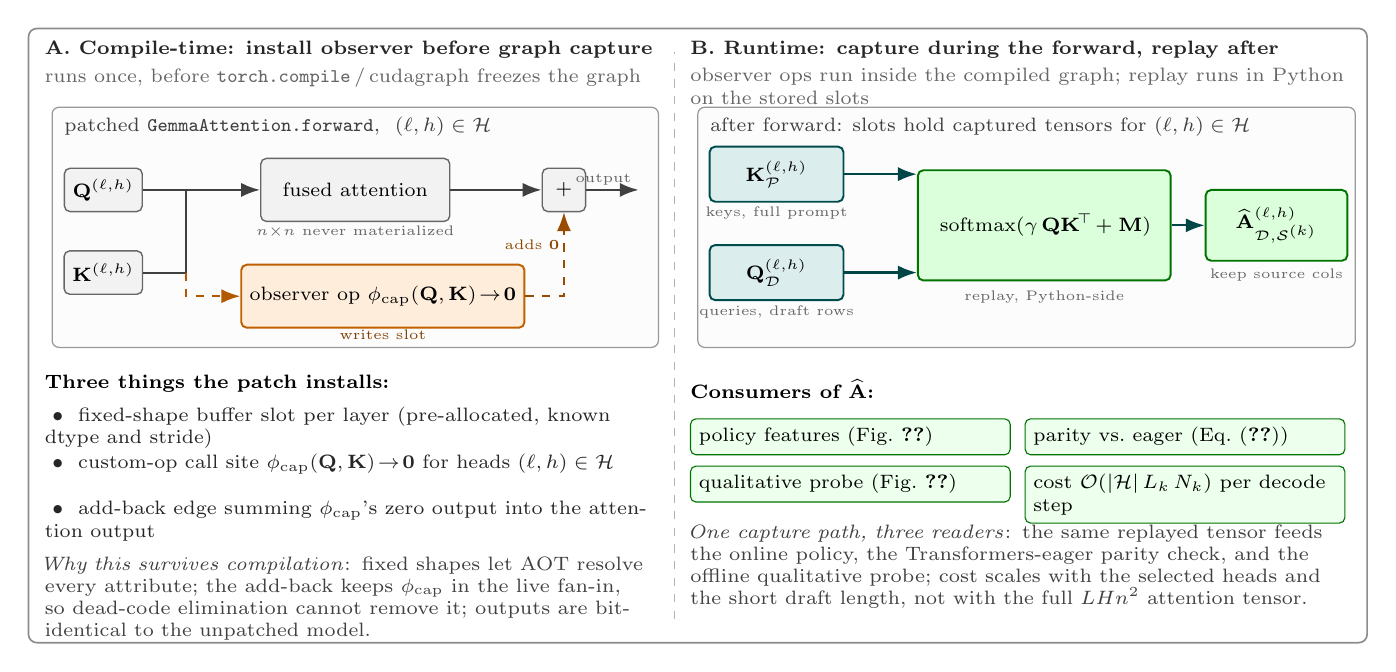
\begin{tikzpicture}[
  x=1cm, y=1cm,
  >={Latex[length=2.4mm]},
  every node/.style={font=\small, inner sep=0pt},
  panel/.style={draw=black!45, rounded corners=3pt, line width=0.6pt, fill=white},
  inner/.style={draw=black!40, line width=0.45pt, rounded corners=2.5pt,
                fill=black!1},
  opnode/.style={draw=black!60, fill=black!5, rounded corners=2pt,
                 line width=0.5pt, inner sep=3pt, font=\scriptsize,
                 align=center},
  obsnode/.style={draw=orange!75!black, fill=orange!14, rounded corners=2pt,
                  line width=0.7pt, inner sep=3pt, font=\scriptsize,
                  align=center},
  bufnode/.style={draw=teal!60!black, fill=teal!14, rounded corners=2pt,
                  line width=0.7pt, inner sep=3pt, font=\scriptsize,
                  align=center},
  outnode/.style={draw=green!45!black, fill=green!14, rounded corners=2pt,
                  line width=0.7pt, inner sep=3pt, font=\scriptsize,
                  align=center},
  tagbox/.style={draw=green!45!black, fill=green!7, rounded corners=2pt,
                 line width=0.4pt, inner sep=3pt, font=\scriptsize, align=left},
  tflow/.style={->, draw=black!75, line width=0.9pt},
  dflow/.style={->, draw=teal!55!black, line width=0.8pt},
  ocap/.style={->, draw=orange!70!black, dashed, line width=0.75pt},
  ozero/.style={->, draw=orange!60!black, dashed, line width=0.65pt},
  wireblk/.style={draw=black!75, line width=0.75pt},
  sectitle/.style={font=\scriptsize\bfseries, align=left, inner sep=0pt},
  sub/.style={font=\scriptsize, align=left, text=black!60, inner sep=0pt},
  tny/.style={font=\tiny, align=left, text=black!55, inner sep=0pt},
  cen/.style={font=\tiny, align=center, text=black!60, inner sep=0pt},
  bullet/.style={font=\scriptsize, align=left, text=black!85, inner sep=0pt},
  prose/.style={font=\scriptsize, align=left, text=black!75, inner sep=0pt},
]

  \def\Wmax{17.00}\def\Hmax{7.80}
  \draw[panel] (0.00,0.00) rectangle (\Wmax,\Hmax);

  \draw[black!30, dashed, line width=0.45pt] (8.20,0.30) -- (8.20,7.50);

  % ========================================================================
  % LEFT: Compile-time setup
  % ========================================================================
  \node[sectitle, text=black!85, anchor=north west] at (0.20,7.65)
    {A.~Compile-time: install observer before graph capture};
  \node[sub, anchor=north west, text width=7.80cm] at (0.20,7.30)
    {runs once, before \texttt{torch.compile}\,/\,cudagraph freezes the graph};

  % --- Inner graph-fragment box ---
  \def\xLL{0.30}\def\xLR{8.00}\def\xLB{3.75}\def\xLT{6.80}
  \draw[inner] (\xLL,\xLB) rectangle (\xLR,\xLT);
  \node[sub, text=black!75, anchor=north west] at (\xLL+0.15,\xLT-0.12)
    {patched \texttt{GemmaAttention.forward},\ \ $(\ell,h)\in\mathcal{H}$};

  % Inputs (stacked)
  \node[opnode, minimum width=0.85cm, minimum height=0.55cm]
    (Q) at (0.95,5.75) {$\mathbf{Q}^{(\ell,h)}$};
  \node[opnode, minimum width=0.85cm, minimum height=0.55cm]
    (K) at (0.95,4.70) {$\mathbf{K}^{(\ell,h)}$};

  % Vertical bus at x=2.00
  \def\Bx{2.00}
  \draw[wireblk] (Q.east) -- (\Bx,5.75);
  \draw[wireblk] (K.east) -- (\Bx,4.70);
  \draw[wireblk] (\Bx,5.75) -- (\Bx,4.70);

  % Fused attention
  \node[opnode, minimum width=2.4cm, minimum height=0.80cm]
    (fused) at (4.15,5.75) {fused attention};
  \node[cen, anchor=north] at (4.15,5.30)
    {$n{\times}n$ never materialized};

  % Observer op
  \node[obsnode, minimum width=3.15cm, minimum height=0.80cm, align=center]
    (obs) at (4.50,4.40)
    {observer op $\phi_{\mathrm{cap}}(\mathbf{Q},\mathbf{K})\!\to\!\mathbf{0}$};
  \node[cen, anchor=north, text=orange!50!black] at (4.50,3.98)
    {writes slot};

  % Sum node
  \node[opnode, minimum width=0.55cm, minimum height=0.55cm]
    (sum) at (6.80,5.75) {$+$};

  % Arrows from bus: clean L-shapes (no diagonals)
  \draw[tflow] (\Bx,5.75) -- (fused.west);
  \draw[ocap] (\Bx,4.70) -- (\Bx,4.40) -- (obs.west);

  % Fused -> sum
  \draw[tflow] (fused.east) -- (sum.west);

  % Observer 0 -> sum (dashed orange, dogleg up)
  \draw[ozero] (obs.east) -- (6.80,4.40) -- (sum.south);
  \node[cen, text=orange!55!black, anchor=east] at (6.75,5.05)
    {adds $\mathbf{0}$};

  % Sum -> output
  \draw[tflow] (sum.east) -- (7.75,5.75);
  \node[cen, anchor=south] at (7.30,5.80) {output};

  % --- Installed items as clean bullet points ---
  \node[sectitle, anchor=north west] at (0.20,3.40)
    {Three things the patch installs:};

  \node[bullet, anchor=north west, text width=7.60cm] at (0.20,3.00)
    {\ $\bullet$\ \ fixed-shape buffer slot per layer (pre-allocated, known
     dtype and stride)};
  \node[bullet, anchor=north west, text width=7.60cm] at (0.20,2.40)
    {\ $\bullet$\ \ custom-op call site
     $\phi_{\mathrm{cap}}(\mathbf{Q},\mathbf{K})\!\to\!\mathbf{0}$ for heads
     $(\ell,h)\in\mathcal{H}$};
  \node[bullet, anchor=north west, text width=7.60cm] at (0.20,1.80)
    {\ $\bullet$\ \ add-back edge summing $\phi_{\mathrm{cap}}$'s zero output
     into the attention output};

  \node[prose, anchor=north west, text width=7.60cm] at (0.20,1.10)
    {\emph{Why this survives compilation}: fixed shapes let AOT resolve every
     attribute; the add-back keeps $\phi_{\mathrm{cap}}$ in the live fan-in,
     so dead-code elimination cannot remove it; outputs are bit-identical to
     the unpatched model.};

  % ========================================================================
  % RIGHT: Per-forward runtime
  % ========================================================================
  \node[sectitle, text=black!85, anchor=north west] at (8.40,7.65)
    {B.~Runtime: capture during the forward, replay after};
  \node[sub, anchor=north west, text width=8.40cm] at (8.40,7.30)
    {observer ops run inside the compiled graph; replay runs in Python on the
     stored slots};

  % --- Inner runtime box ---
  \def\xRL{8.50}\def\xRR{16.85}\def\xRB{3.75}\def\xRT{6.80}
  \draw[inner] (\xRL,\xRB) rectangle (\xRR,\xRT);
  \node[sub, text=black!75, anchor=north west] at (\xRL+0.15,\xRT-0.12)
    {after forward: slots hold captured tensors for $(\ell,h)\in\mathcal{H}$};

  % Captured K
  \node[bufnode, minimum width=1.70cm, minimum height=0.70cm]
    (bK) at (9.50,5.95) {$\mathbf{K}^{(\ell,h)}_{\mathcal{P}}$};
  \node[cen, anchor=north] at (9.50,5.54) {keys, full prompt};

  % Captured Q
  \node[bufnode, minimum width=1.70cm, minimum height=0.70cm]
    (bQ) at (9.50,4.70) {$\mathbf{Q}^{(\ell,h)}_{\mathcal{D}}$};
  \node[cen, anchor=north] at (9.50,4.29) {queries, draft rows};

  % Replay op: shorter, wrapped formula so the box width is predictable
  \node[outnode, text width=3.00cm, align=center, minimum height=1.40cm]
    (replay) at (12.90,5.30)
    {$\mathrm{softmax}(\gamma\,\mathbf{Q}\mathbf{K}^{\!\top}\!+\mathbf{M})$};
  \node[cen, anchor=north] at (12.90,4.48) {replay, Python-side};

  % Slice output
  \node[outnode, minimum width=1.80cm, minimum height=0.90cm]
    (slice) at (15.85,5.30)
    {$\widehat{\mathbf{A}}^{(\ell,h)}_{\mathcal{D},\mathcal{S}^{(k)}}$};
  \node[cen, anchor=north] at (15.85,4.75) {keep source cols};

  % Edges
  \draw[dflow] (bK.east) -- (replay.west |- bK);
  \draw[dflow] (bQ.east) -- (replay.west |- bQ);
  \draw[dflow] (replay.east) -- (slice.west);

  % --- Consumer tags (with room above the tagbox row) ---
  \node[sectitle, anchor=north west] at (8.40,3.35)
    {Consumers of $\widehat{\mathbf{A}}$:};

  \node[tagbox, anchor=north west, text width=3.85cm] at (8.40,2.85)
    {policy features (Fig.~\ref{fig:policy-pipeline})};
  \node[tagbox, anchor=north west, text width=3.85cm] at (12.65,2.85)
    {parity vs.\ eager (Eq.~\eqref{eq:parity})};
  \node[tagbox, anchor=north west, text width=3.85cm] at (8.40,2.25)
    {qualitative probe (Fig.~\ref{fig:mt-selective-reconstruction})};
  \node[tagbox, anchor=north west, text width=3.85cm] at (12.65,2.25)
    {cost $\mathcal{O}(|\mathcal{H}|\,L_k\,N_k)$ per decode step};

  \node[prose, anchor=north west, text width=8.20cm] at (8.40,1.50)
    {\emph{One capture path, three readers}: the same replayed tensor feeds
     the online policy, the Transformers-eager parity check, and the offline
     qualitative probe; cost scales with the selected heads and the short
     draft length, not with the full $LHn^2$ attention tensor.};

\end{tikzpicture}
}%
\caption{\textbf{Compile-safe observer lifecycle on the deployed vLLM path.}
\emph{Left (A), once, before graph capture:} the forward of
\texttt{GemmaAttention} is patched so that for each selected head
$(\ell,h)\in\mathcal{H}$ the query and key tensors also pass through an
observer custom op $\phi_{\mathrm{cap}}$ (dashed orange side path). The op
writes the selected slices into fixed-shape, pre-allocated slots and returns
a zero tensor that is added back into the attention output; this keeps the op
in the live fan-in of the graph so the compiler cannot dead-code-eliminate
it, while the numerical output of the layer is unchanged.
\emph{Right (B), every forward:} after the compiled forward finishes, the
observer slots hold $\mathbf{K}^{(\ell,h)}_{\mathcal{P}}$ for the full prompt
and $\mathbf{Q}^{(\ell,h)}_{\mathcal{D}}$ for the draft rows; a short
Python-side replay reapplies the module scaling and the same prompt/suffix
masks used by the deployed attention kernel, then keeps the source columns to
yield the selective block
$\widehat{\mathbf{A}}^{(\ell,h)}_{\mathcal{D},\mathcal{S}^{(k)}}$ that feeds
the policy, the parity check against an uncompiled Transformers reference,
and the qualitative probe.}
\label{fig:observer-lifecycle}
\end{figure*}


\paragraph{Compile-safe capture and replay.}
Figure~\ref{fig:appendix-observer-lifecycle} replaces the buffer algebra. The
observer is installed before compilation, one slot per layer, so the compiled
graph never encounters missing attributes. During the fused forward, it records
only fixed-shape prompt-key and draft query/key tensors for the selected head
subset; this is why the capture path stays compile-safe. The custom op is
numerically inert, but its zero-valued return is added back into the attention
output so the compiler cannot dead-code-eliminate it. After the decode step,
the stored buffers are sufficient to rebuild prompt-side logits, suffix-side
logits, and finally the same source-restricted rows that the policy consumes.

\paragraph{Qualitative reconstruction example.}
Figure~\ref{fig:mt-selective-reconstruction} instantiates the full
reconstruction stack on a text-only MT probe: the exact prompt
partition seen by the decoder is shown, reconstructed token-level rows are
aggregated to the word level for readability, and the four-way provenance
accounting is kept visible for every drafted word.
\paragraph{Residual provenance in decoder-only AlignAtt.}
Unlike encoder--decoder AlignAtt, the replayed decoder-only rows are not normalized over the source alone: attention can also land on the accepted target prefix, the rest of the prompt template, and the speculative suffix. On the French qualitative probe bank used to mine Fig.~\ref{fig:mt-selective-reconstruction} (78 scored prefix-continuation probes on an NVIDIA A40), drafted target units allocate on average 9\% to accessible source tokens, 8\% to still-inaccessible source tokens, 81\% to non-source prompt positions (system/template plus accepted prefix), and 2\% to the speculative suffix. Restricting to the target units that AlignAtt actually accepts shifts these shares to 14\%/1\%/83\%/2\%. These residual masses are therefore not implementation noise but a structural difference from standard AlignAtt.


\paragraph{Numerical parity.}
Let $\mathbf{A}^{(\mathrm{TF})}$ denote the reference attention tensor produced
by an uncompiled Transformers forward on the identical prompt. On a curated
parity set, we observe
\begin{equation}
  \begin{aligned}
    \|\Delta\mathbf{A}\|_\infty &\leq 1.2 \times 10^{-2}, \\
    \|\Delta\mathbf{A}\|_1 / (nL_k) &\leq 4 \times 10^{-4},
  \end{aligned}
  \label{eq:parity}
\end{equation}
with bit-identical acceptance decisions between the eager and compiled paths.
The observer is therefore not just fast enough to keep, but faithful enough to
support controlled MT ablations.

\section{Additional ASR Analyses}
\label{sec:appendix-asr}

This appendix collects the all-Gemma ASR analyses that informed the final
system choice but are no longer central to the retained submission narrative.

\paragraph{Why the submitted system keeps Qwen3 forced ASR.}
Table~\ref{tab:asr-compare} compares the dedicated Qwen3 forced aligner with
the discarded Gemma AlignAtt ASR path on the diagnostic clip
\texttt{ccpXHNfaoy}. The direction is unambiguous: Qwen3 forced is better in
WER, boundary lag, and wall-clock RTF. That is why the submitted system keeps
Qwen3 forced ASR rather than pushing the single-substrate idea into the final
submission.

\begin{table}[t]
\centering
\small
\setlength{\tabcolsep}{4pt}
\begin{tabular}{lcc}
\toprule
 & Qwen3 forced & Gemma AlignAtt \\
\midrule
WER $\downarrow$                 & $0.113$ & $0.269$ \\
CER $\downarrow$                 & $0.046$ & $0.122$ \\
Boundary F1 $\pm$3w $\uparrow$   & $0.878$ & $0.042$ \\
Mean $|$lag$|$ (s) $\downarrow$  & $0.145$ & $0.403$ \\
Load time (s)                    & $63.7$  & $123.0$ \\
RTF (wall-clock) $\downarrow$    & $0.306$ & $0.628$ \\
\bottomrule
\end{tabular}
\caption{\textbf{ASR alignment comparison on \texttt{ccpXHNfaoy} (360 s).}
Qwen3 forced remains clearly stronger than the discarded Gemma AlignAtt ASR
path on both boundary quality and runtime.}
\label{tab:asr-compare}
\end{table}

\paragraph{Verified 21-clip ASR reference row.}
Across the tracked 21-clip dev set, the verified Qwen3 forced row provides a
stable point of comparison for the MT-side submission stack:

\begin{table}[t]
\centering
\small
\begin{tabular}{lc}
\toprule
Metric & Qwen3 forced (LA) \\
\midrule
Mean WER $\downarrow$         & $0.092$ \\
Mean CER $\downarrow$         & $0.042$ \\
BLEU $\uparrow$               & $74.82$ \\
chrF $\uparrow$               & $90.81$ \\
LongYAAL CU (ms) $\downarrow$ & $865.7$ \\
LongYAAL CA (ms) $\downarrow$ & $672.7$ \\
\bottomrule
\end{tabular}
\caption{\textbf{Verified aggregate Qwen3 forced ASR reference} on the 21-clip
dev set, evaluated in the same ASR-as-MT setup used during development.}
\label{tab:asr-21clip}
\end{table}

\paragraph{Gemma AlignAtt ASR is feasible but not competitive.}
We also swept Gemma-ASR streaming configurations and head-fusion rules to
expose its latency/quality frontier. The conclusion is short: the path runs
end-to-end and produces reasonable transcripts, but no sub-one-second
operating point we tried approaches the quality or boundary lag of the
dedicated Qwen3 forced aligner, and the only fusion change that reliably
helped was switching from mean pooling to a median of per-head argmax
positions. We therefore report Gemma AlignAtt ASR only as an exploratory
baseline here, not as a candidate submission.

\end{document}
